
\documentclass[11pt]{amsart}

\usepackage{amsmath}
\usepackage{amssymb}
\usepackage{amsthm}
\usepackage{mathtools}
\usepackage{enumitem}
%\usepackage{thmtools}
\usepackage{hyperref}
\hypersetup{hypertexnames=false}
\usepackage[nameinlink,noabbrev]{cleveref}
\usepackage{booktabs}
\usepackage{graphicx}
\usepackage{xcolor}
\usepackage{tikz}
\usetikzlibrary{shapes.geometric, arrows.meta, positioning}


% ---- Theorem environments ----
\theoremstyle{plain}
\newtheorem{theorem}{Theorem}
\newtheorem{proposition}[theorem]{Proposition}
\newtheorem{lemma}[theorem]{Lemma}
\newtheorem{corollary}[theorem]{Corollary}
\newtheorem{claim}[theorem]{Claim}

\theoremstyle{definition}
\newtheorem{definition}[theorem]{Definition}
\newtheorem{assumption}[theorem]{Assumption}
\newtheorem{example}[theorem]{Example}

\theoremstyle{remark}
\newtheorem{remark}[theorem]{Remark}

% ---- Macros ----
\newcommand{\cond}{\operatorname{cond}}
\newcommand{\KL}{D_{\operatorname{KL}}}
\newcommand{\E}{\mathbb{E}}
\newcommand{\Var}{\operatorname{Var}}
\newcommand{\Cov}{\operatorname{Cov}}
\newcommand{\tr}{\operatorname{Tr}}
\newcommand{\diag}{\operatorname{diag}}

\newcommand{\Range}{\operatorname{Range}}
\newcommand{\Span}{\operatorname{span}}
\newcommand{\id}{\mathrm{id}}
% \newcommand{\TODO}[1]{\textcolor{red}{[TODO: #1]}} % removed for submission

% ---- Cleveref names ----
\crefname{theorem}{theorem}{theorems}
\Crefname{theorem}{Theorem}{Theorems}
\crefname{proposition}{proposition}{propositions}
\Crefname{proposition}{Proposition}{Propositions}
\crefname{lemma}{lemma}{lemmas}
\Crefname{lemma}{Lemma}{Lemmas}
\crefname{corollary}{corollary}{corollaries}
\Crefname{corollary}{Corollary}{Corollaries}
\crefname{claim}{claim}{claims}
\Crefname{claim}{Claim}{Claims}
\crefname{definition}{definition}{definitions}
\Crefname{definition}{Definition}{Definitions}
\crefname{assumption}{assumption}{assumptions}
\Crefname{assumption}{Assumption}{Assumptions}
\crefname{example}{example}{examples}
\Crefname{example}{Example}{Examples}
\crefname{remark}{remark}{remarks}
\Crefname{remark}{Remark}{Remarks}
\crefname{equation}{Eq.}{Eqs.}
\Crefname{equation}{Equation}{Equations}
\crefname{figure}{fig.}{figs.}
\Crefname{figure}{Fig.}{Figs.}
\crefname{table}{table}{tables}
\Crefname{table}{Table}{Tables}
\crefname{section}{Sec.}{Secs.}
\Crefname{section}{Section}{Sections}

\title[Singular Gaussian Conditioning in Hilbert Space]{Singular Gaussian Conditioning in Hilbert Space: Schur Residuals, Fisher Scaling, and Cameron--Martin Energy}

\author{Lucia Yizi Zhang}
\thanks{L.~Y.~Zhang is an Independent Researcher (e-mail: lucia.zhang.research@outlook.com, ORCID: \href{https://orcid.org/0009-0005-3528-7747}{0009-0005-3528-7747}). Manuscript received May 2026. Code and supplemental materials are archived at \url{https://github.com/OstensibleParadox/singular-causal-interventions}.}

\begin{document}

    % ============================================================
    %  ABSTRACT
    % ============================================================
    \begin{abstract}
        We investigate infinite-dimensional Gaussian models under singular hyperplane conditioning. As the regularized conditioning strength $\lambda \to \infty$, the conditional laws exit the equivalent-measure manifold of the reference prior due to the Feldman–H\'{a}jek dichotomy. To resolve this singularity without invoking unbounded operators, we introduce an inverse-free variational Schur projection that reduces the infinite-dimensional problem to its canonical normal form. We prove that this Schur residual guarantees an exact target variance calibration $\Sigma_{\lambda,kk} = \varepsilon_0/(2\lambda^2)$ alongside a projection residual $R_\lambda = O(\lambda^{-6})$. By defining a local blow-up coordinate $b = \lambda(x_K^* - m_{\lambda,K})$, we demonstrate that the rescaled Fisher tensor admits a Schur-precision expansion. The leading term constitutes a flat Mahalanobis Fisher scaling, while the first nontrivial correction—extracted via a Fenchel-dual variational formulation—is precisely the Cameron–Martin Renormalized Fisher Information Metric (RFIM) residue. When applied to an elliptic Gaussian field, this residue specializes to the Sobolev–Dirichlet energy. These results characterize the exact differential geometry of singular boundaries purely through the algebraic invariants of the Hilbert-space Gaussian condition.
    \end{abstract}

    \keywords{Singular conditioning; Gaussian measures; Cameron--Martin space; Schur complement; Hilbert dynamics; trace covariance; finite-part regularization; Galerkin approximation; Fisher scaling; Renormalized Fisher Information Metric; Sobolev--Dirichlet energy}

    \maketitle

    % ============================================================
    %  §1  INTRODUCTION
    % ============================================================
    \section{Introduction}
    \label{sec:intro}

    Singular hyperplane conditioning arises when one approximates a hard constraint $X_k = x_k^*$ by a calibrated family of linear dynamics with regularization parameter $\lambda$, followed by the limit $\lambda \to \infty$. In finite-dimensional Gaussian dynamics, the resulting conditional covariance is described by an ordinary Schur complement. In infinite-dimensional Hilbert-space dynamics, this algebraic description breaks down: stationary covariance operators are trace-class and compact, hence their restrictions do not admit bounded global inverses.

    However, when the state space is an infinite-dimensional separable Hilbert space---as arises in stochastic evolution equations \cite{daprato2014stochastic} and functional linear processes \cite{bosq2000linear}---the standard algebraic machinery collapses. The passage from a smooth restoring control of strength $\lambda$ to the discrete topological cut $\lambda \to \infty$ constitutes a singular perturbation limit \cite{pavliotis2008multiscale} in which three fundamental obstructions emerge:
    \begin{enumerate}
        \item \textbf{Unbounded Precision Operators.} The stationary covariance operator is trace-class and compact \cite{daprato2014stochastic}, so its restriction to the free coordinates lacks a bounded global inverse. The Schur complement cannot be defined via operator inversion. Spectral properties of block operator Schur complements have been studied extensively \cite{tretter2008spectral,gerhat2024schur}, and the variational ``shorted operator'' perspective \cite{anderson1975shorted} addresses positive-operator compressions. However, these results address spectral enclosures and operator shorting without establishing a direct connection to statistical projection residuals under singular Gaussian conditioning.
        \item \textbf{Hyperplane Disintegration Singularity.} Conditioning a Radon Gaussian measure on a codimension-1 hyperplane $X_k = x_k^*$ produces a measure supported on a set of prior probability zero \cite{bogachev1998gaussian}. The joint Kullback--Leibler divergence between the exact conditioned law and any non-degenerate prior is $+\infty$.
        \item \textbf{Feldman--H\'{a}jek Critical Boundary.} The Feldman--H\'{a}jek dichotomy \cite{feldman1958equivalence,hajek1958property,bogachev1998gaussian} implies that two Gaussian measures on a separable Hilbert space are either mutually absolutely continuous or mutually singular. In the Bayesian inverse-problem literature \cite{stuart2010inverse}, only soft observations with positive-definite noise (which are algebraically equivalent to Tikhonov regularization \cite{franklin1970well}) preserve equivalence; hard conditioning forces singularity. Regularized Kullback--Leibler approximations for infinite-dimensional measures \cite{pinski2015kullback} provide a finite surrogate in the equivalent regime, but the hard coordinate conditioning lies beyond this regime.
    \end{enumerate}

    To resolve the geometry of the singularity, we construct a tangent blow-up microscope by defining the scaled local coordinate $b \coloneqq \lambda(x_k^* - m_{\lambda,k})$. Instead of ad hoc singularity subtraction, we investigate the limit through this tangent blow-up coordinate geometry. Pulling the Fisher metric back to the regularized singular conditioning boundary reveals an exact hierarchical expansion. By combining the coordinate pull-back Jacobian $\lambda^{-2}$ with the exact Schur variance calibration $S_{k,\lambda} = \varepsilon_0/(2\lambda^2) - R_\lambda$ and the Woodbury matrix identity, the rescaled joint Fisher metric tensor cleanly bifurcates into distinct analytical strata in the blow-up limit:
    \begin{enumerate}
        \item \textbf{0th-order normal geometry (Displacement Flatness)}: The non-degenerate 0th-order term defines a flat Mahalanobis tangent cone $2\varepsilon_0^{-1}$, structurally preserving the displacement-flatness of Gaussian location families without manufacturing spurious boundary curvature.
        \item \textbf{1st-order horizontal metric limit (Schur-precision correction)}: Strikingly, the 1st-order $O(\lambda^{-4})$ perturbative geometry isolates the Cameron--Martin energy of the horizontal lift of the unobserved bulk fibers, yielding exactly the renormalized Fisher information metric (RFIM) limit $\|a_{Ik}\|_{Q_0^{-1}}^2$.
    \end{enumerate}

    The cancellation mechanism has four layers. First, exact variance normalization fixes the target variance at $\Sigma_{\lambda,kk}=\varepsilon_0/(2\lambda^2)$. Second, the block-decoupling constraint gives an exact block-Lyapunov resolvent for the off-diagonal drift coupling covariance. Third, Cameron--Martin admissibility converts this coupling into an inverse-free variational Schur subtraction of order $O(\lambda^{-6})$, producing the Schur pole $S_{k,\lambda}^{-1}=(2/\varepsilon_0)\lambda^2+O(\lambda^{-2})$. Fourth, in the Gaussian case, the Dirac-conditioning singularity is removed by a finite-part regularization, leaving the bounded action $\mathfrak{J}_\lambda=b_k^2/\varepsilon_0+O(\lambda^{-4})$ (exactly zero under decoupled centering). Every technical tool---Cameron--Martin energy, Douglas range inclusion \cite{douglas1966majorization}, Gr\"umm ideal convergence \cite{simon2005trace}, Radon disintegration, and Feldman--H\'{a}jek equivalence---serves this single mechanical chain.

    We resolve these singular limits by establishing a unified mathematical hierarchy:
    \begin{enumerate}
        \item \textbf{Projection Residual Scaling Base Theorem:} For any linear stationary process with finite second moments whose covariance satisfies the Lyapunov equation, we prove a Hilbert-space projection residual scaling (\Cref{thm:inf_cancellation}) using covariance-energy forms. The target $L^2$-projection residual, equivalently the LMMSE residual, satisfies $S_{k,\lambda} = \varepsilon_0/(2\lambda^2) - R_\lambda$, meaning its inverse scales as $S_{k,\lambda}^{-1} = (2/\varepsilon_0)\lambda^2 + O(\lambda^{-2})$.
        \item \textbf{Gaussian Conditional Extension and Schur-Precision Expansion:} Under the additional assumption of Gaussian Radon laws, we enhance this base result to a conditional analysis. We construct the conditional predictor via the Cameron--Martin space of the bulk covariance, avoiding unbounded inverse operators. Gaussian disintegration yields exact target coordinate zeros under the conditioned evidence. We define the Gaussian renormalized finite-part functional $\mathfrak{J}_\lambda$ using a Dirac mollification scheme, and prove it converges to $b_k^2/\varepsilon_0 + O(\lambda^{-4})$. If the system is decoupled and the evidence is centered, the functional vanishes exactly for all $\lambda > 0$. We then demonstrate that the rescaled joint Fisher metric tensor admits a clean asymptotic expansion where the 0th-order normal geometry is flat and the 1st-order perturbation isolates the Cameron--Martin coupling energy of the off-diagonal drift.
    \end{enumerate}

    Our approach differs fundamentally from the Bayesian inverse-problem literature \cite{stuart2010inverse}, in which soft observations with positive-definite noise preserve Gaussian equivalence. We study the measure-theoretic structure of the singular conditioning limit itself---specifically, the collapse of the joint information divergence on the underlying operator algebra as the regularization parameter diverges.

    \subsection{Related work and positioning}
    \label{sec:related}

    \paragraph{Equivalent-measure manifolds and singular boundaries.}
    The classical extension of information geometry to infinite-dimensional spaces \cite{amari2000methods,pistone1995infinite,newton2012infinite} constructs statistical manifolds on the set of probability measures equivalent (i.e., mutually absolutely continuous) to a given reference measure. This equivalent-measure requirement is both natural and restrictive: it guarantees that the Fisher metric is well-defined and the manifold structure is smooth, but it fails precisely when the model enters a mutually singular regime. Hard hyperplane conditioning ($\lambda \to \infty$) produces such a regime: the conditioned measures converge to a Dirac distribution on the target coordinate and exit the equivalence class of the reference Gaussian law. The tangent blow-up coordinate extracts the rescaled metric limit from the divergent KL boundary, acting as a renormalization at the edge of the equivalent-measure manifold.

    \paragraph{The Feldman--H\'{a}jek measure-class wall.}
    The Feldman--H\'{a}jek theorem \cite{feldman1958equivalence,hajek1958property,bogachev1998gaussian} establishes a sharp dichotomy for Gaussian measures on separable Hilbert spaces: two Gaussian laws are either equivalent or mutually singular, with no intermediate case. In Bayesian inverse problems, \cite{stuart2010inverse} shows that positive observational noise keeps the posterior in the equivalent regime; zero-noise hard conditioning exits that regime. The standard workaround is to force additive observation noise into the model, preserving absolute continuity at the cost of never reaching the exact conditioning limit. Our construction takes a different route: the tangent blow-up isolates the non-degenerate geometric limit while preserving the Cameron--Martin energy structure of the coupling, without injecting artificial noise.

    \paragraph{Transport geometry and Bures--Wasserstein limits.}
    Infinite-dimensional Gaussian measures that are mutually singular can still be compared via optimal transport distances. The Wasserstein geometry of Gaussian measures \cite{takatsu2011wasserstein} and the Bures--Wasserstein distance between covariance operators \cite{bhatia2019bures} provide global metrics that do not require absolute continuity; for background on optimal transport and gradient flows in metric spaces, see \cite{villani2009optimal}. The geometry developed here is complementary: the tangent blow-up metric governs the boundary normal geometry and horizontal lift of singular evidence values (\Cref{sec:fisher_geometry}), while the Bures--Wasserstein metric governs bulk covariance relaxation. The present paper does not use any Wasserstein gradient-flow identity.

    \paragraph{Distinction from singular learning theory.}
    \cite{watanabe2009algebraic} develops a theory of singular statistical models in which the Fisher information matrix degenerates due to parameter redundancy (the parameter-to-law map has an algebraic singularity). The singularity studied here is fundamentally different: the parameterization remains linear and the model Gaussian, but the limiting measures leave the common absolutely continuous class under hard conditioning. Watanabe's tools---resolution of singularities, real log-canonical thresholds, learning coefficients---address algebraic degeneracy of the Fisher matrix on a finite-dimensional parameter space. Our tangent blow-up addresses the measure-theoretic singularity of a KL divergence that diverges because the conditioned measures become mutually singular in infinite dimensions.

    \subsection{Organization of the Paper}
    We organize the paper as follows. \Cref{sec:setup} defines the operator model and the variance normalization. \Cref{sec:infdim} establishes the Hilbert-space Schur residual scaling. \Cref{sec:gaussian_zero} details the Gaussian conditional extension and the renormalized finite-part functional. \Cref{sec:fisher_geometry} establishes the rescaled Fisher tensor and the Schur-precision tangent blow-up expansion. \Cref{sec:spde} demonstrates the framework on an infinite-dimensional Gaussian field model, interpreting the RFIM as a Dirichlet connection energy. \Cref{sec:discussion} discusses non-Gaussian limitations. \Cref{sec:conclusion} concludes. Proofs are given in \Cref{app:block_cumulant_analysis,app:gaussian_lift,sec:formal:proofs}; numerical diagnostics and Galerkin verification in \Cref{app:experiments}.
    \section{Operator Model and Exact Variance Normalization}
    \label{sec:setup}

    \subsection{Operator Dynamics and Regularized Conditioning}
    \label{sec:setup:dynamics}

    We model the continuous-time dynamics as stochastic evolution on a separable Hilbert space $\mathcal{H}$ \cite{daprato2014stochastic}:
    \begin{equation}
        \label{eq:stochastic_evolution}
        dX_t = \mathcal{A} X_t \, dt + \mathcal{D}^{1/2} dW_t
    \end{equation}
    where $\mathcal{A}$ is the drift operator and $\mathcal{D}$ is the trace-class diffusion operator. We decompose the Hilbert space as $\mathcal{H} = \mathcal{H}_k \oplus \mathcal{H}_I$, where $\mathcal{H}_k \coloneqq \mathbb{R}\phi_k$ is the one-dimensional target coordinate subspace, and $\mathcal{H}_I \coloneqq \mathcal{H}_k^\perp$ is the free bulk subspace. Let $\Pi_k \coloneqq \phi_k \otimes \phi_k$ and $\Pi_I \coloneqq I - \Pi_k$ be the corresponding orthogonal projections.

    To approximate the exact point conditioning $X_k = x_k^*$, we sever all incoming target-coordinate edges and apply a regularization parameter $\lambda > 0$.

    \begin{definition}[Calibrated Approximating Dynamics Family]
        \label{def:soft_do}
        The regularized conditioning operator of strength $\lambda > 0$ at node $X_k$ acts on the operator dynamics \eqref{eq:stochastic_evolution} by modifying both the drift and the diffusion:
        \begin{equation}
            \label{eq:soft_do_sde}
            \mathcal{A}^{(\lambda)} \coloneqq \mathcal{A}_{\cond} - \lambda \Pi_k, \qquad
            \mathcal{D}^{(\lambda)} \coloneqq \mathcal{D}_{\cond} + d_\lambda \Pi_k
        \end{equation}
        where $\mathcal{A}_{\cond}$ is the block drift operator with all incoming target-coordinate edges severed ($\Pi_k \mathcal{A}_{\cond} = 0$), $\mathcal{D}_{\cond}$ has target-coordinate noise severed, and $d_\lambda > 0$ is the local diffusion variance of the target coordinate at regularization strength $\lambda$. In the SDE, this corresponds to:
        \begin{equation}
            \label{eq:soft_do_sde_general}
            dX_{k,t} = -\lambda (X_{k,t} - x_k^*) dt + \sqrt{d_\lambda}\, dW_{k,t}.
        \end{equation}
    \end{definition}

    \subsection{Exact Variance Normalization}
    \label{sec:setup:calibration}

    The block-decoupled structure under the regularized dynamics yields:
    \begin{equation}
        \mathcal{A}^{(\lambda)}=
    \begin{pmatrix}-\lambda&0\\a_{Ik}&\mathcal{A}_{II}\end{pmatrix},\qquad
        \mathcal{D}^{(\lambda)}=
    \begin{pmatrix}d_\lambda&0\\0&D_{II}\end{pmatrix},
    \end{equation}
    where $a_{Ik} \coloneqq \mathcal{A}_{Ik} \phi_k \in \mathcal{H}_I$ represents the off-diagonal drift coupling.
    Let $\Sigma_\lambda$ denote the stationary covariance operator under regularization strength $\lambda$, solving the Lyapunov equation:
    \begin{equation}
        \mathcal{A}^{(\lambda)}\Sigma_\lambda + \Sigma_\lambda(\mathcal{A}^{(\lambda)})^* + \mathcal{D}^{(\lambda)} = 0.
    \end{equation}
    The target block $kk$ decouples completely from the free coordinates, yielding the exact scalar equation:
    \begin{equation}
        -2\lambda\Sigma_{\lambda,kk} + d_\lambda = 0 \quad \Longrightarrow \quad \Sigma_{\lambda,kk} = \frac{d_\lambda}{2\lambda}.
    \end{equation}

    \begin{proposition}[Exact Variance Normalization]
        \label{prop:exact_calibration}
        To maintain a physical target noise scale $\varepsilon_0 > 0$ independent of the auxiliary parameter $\lambda$ under the singular limit, we define the exact variance normalization condition:
        \begin{equation}
            \lambda^2 \Sigma_{\lambda,kk} \equiv \frac{\varepsilon_0}{2} \quad \text{for all } \lambda > 0,
        \end{equation}
        which uniquely requires:
        \begin{equation}
            d_\lambda = \frac{\varepsilon_0}{\lambda} \quad \text{for every } \lambda > 0.
        \end{equation}
        Substitution of this target diffusion scaling yields the calibrated approximating dynamics:
        \begin{equation}
            dX_{k,t} = -\lambda (X_{k,t} - x_k^*) dt + \sqrt{\varepsilon_0 / \lambda}\, dW_{k,t}.
        \end{equation}
    \end{proposition}

    All subsequent results are stated for this calibrated family.

    \begin{definition}[Schur LMMSE Invariant]
        \label{def:schur_invariant}
        Let $S_{k,\lambda} \coloneqq \|X_k - P_{\mathcal{M}_I} X_k\|_{L^2}^2$ represent the linear minimum mean squared error (LMMSE) residual of the target coordinate $X_k$ on the closed linear span $\mathcal{M}_I$ of the free coordinates $X_I$. The \emph{Schur LMMSE invariant} $m_2^{\mathrm{Schur}}$ is defined as:
        \begin{equation}
            \label{eq:m2_schur_definition}
            m_2^{\mathrm{Schur}} \coloneqq \lim_{\lambda\to\infty} \lambda^2 S_{k,\lambda}.
        \end{equation}
    \end{definition}

    \subsection{Operator Setup and Assumptions}
    \label{sec:setup:assumptions}

    We state the operator-theoretic assumptions that make the limit passage independent of the Galerkin dimension.

    \begin{definition}[Drift Operator with Volterra Perturbation]
        \label{def:drift_operator}
        A drift operator on a separable Hilbert space $\mathcal{H}$ is an operator of the form $\mathcal{A} = \mathcal{A}_0 + \mathcal{K}$, where:
        \begin{enumerate}
            \item[(i)] $\mathcal{A}_0: \operatorname{dom}(\mathcal{A}_0) \subset \mathcal{H} \to \mathcal{H}$ is a closed, densely defined, dissipative operator that generates a strongly continuous contraction semigroup $(e^{t\mathcal{A}_0})_{t \ge 0}$ on $\mathcal{H}$, satisfying $\|e^{t\mathcal{A}_0}\| \le e^{-\alpha t}$ for some spectral gap $\alpha > 0$.
            \item[(ii)] $\mathcal{K}: \mathcal{H} \to \mathcal{H}$ is a compact Volterra operator with spectral radius $\rho(\mathcal{K}) = 0$.
            \item[(iii)] The full operator $\mathcal{A} = \mathcal{A}_0 + \mathcal{K}$ generates a strongly continuous semigroup $(e^{t\mathcal{A}})_{t \ge 0}$ by the bounded perturbation theorem, and this semigroup remains exponentially stable: $\|e^{t\mathcal{A}}\| \le M e^{-\beta t}$ for some $M \ge 1$, $\beta > 0$.
        \end{enumerate}
        In finite dimensions ($\mathcal{H} = \mathbb{R}^n$), $\mathcal{A}_0$ reduces to the Hurwitz drift matrix $A$ and $\mathcal{K} = 0$.
    \end{definition}

    \begin{definition}[Trace-Class Noise and Covariance]
        \label{def:trace_class}
        Let $\mathcal{S}_1(\mathcal{H})$ denote the Banach space of trace-class (nuclear) operators on $\mathcal{H}$ equipped with the trace norm $\|T\|_{\mathcal{S}_1} \coloneqq \tr(|T|) = \sum_{i=1}^\infty \langle \phi_i, (T^*T)^{1/2} \phi_i \rangle < \infty$.
        \begin{enumerate}
            \item[(i)] The diffusion operator $\mathcal{D}: \mathcal{H} \to \mathcal{H}$ is positive, self-adjoint, and belongs to $\mathcal{S}_1(\mathcal{H})$.
            \item[(ii)] Assuming the pair $(\mathcal{A}, \mathcal{D}^{1/2})$ is controllable, the stationary covariance operator $\Sigma: \mathcal{H} \to \mathcal{H}$ is the unique strictly positive, self-adjoint, trace-class solution to the operator Lyapunov equation:
            \begin{equation}
                \label{eq:op_lyapunov}
                \mathcal{A}\Sigma + \Sigma\mathcal{A}^* + \mathcal{D} = 0
            \end{equation}
            which is given by the convergent Bochner integral
            \[
            \Sigma = \int_0^\infty e^{t\mathcal{A}} \mathcal{D} e^{t\mathcal{A}^*} dt.
            \]
        \end{enumerate}
    \end{definition}

    \begin{assumption}[Core Analytical Assumptions for Singular Hyperplane Conditioning]
        This work relies on two core analytical assumptions regarding the target-coordinate cut and the outgoing coupling:
        \begin{enumerate}
            \item[(i)] \textbf{Linear Second-Moment Channel:} \label{assum:linear_second_moment} A centered linear stationary process on $\mathcal{H}=\mathcal{H}_k\oplus \mathcal{H}_I$ has finite second moments and covariance solving \Cref{eq:op_lyapunov}. The block-decoupling constraint zeroes all incoming target drift and cross-noise, so that $\mathcal{A}_{kI}=\mathcal{D}_{kI}=\mathcal{D}_{Ik}=0$ and $\mathcal{A}_{kk}=-\lambda$. The target diffusion $\mathcal{D}_{kk}=\varepsilon_0/\lambda$ is the unique scaling determined by the exact variance normalization (Proposition~\ref{prop:exact_calibration}). The free noise is independent of the local target noise. (Gaussianity is not assumed).
            \item[(ii)] \textbf{Cameron--Martin Stability of Off-Diagonal Drift Coupling:} \label{assum:cm_stability} Let $Q_0\coloneqq\Sigma_{II}^{(0)}$ denote the free-block covariance produced by the free noise under block decoupling, and let $H_{Q_0}\coloneqq\operatorname{Range}(Q_0^{1/2})$ with the energy norm $|u|_{Q_0}\coloneqq\|Q_0^{-1/2}u\|_{\mathcal{H}_I}$. The outgoing vector $a_{Ik}\coloneqq\mathcal{A}_{Ik}\phi_k$ belongs to $H_{Q_0}$, and $e^{t\mathcal{A}_{II}}$ restricts to a strongly continuous exponentially stable semigroup on $H_{Q_0}$:
            \begin{equation}
                \|e^{t\mathcal{A}_{II}}\|_{\mathcal{L}(H_{Q_0})} \le M e^{-\omega t},\qquad t\ge0,
            \end{equation}
            for constants $M\ge1$ and $\omega>0$ independent of $\lambda$.
        \end{enumerate}
        \vspace{1mm}
        \noindent\textit{Intuitive Explanation:} Part (i) states that the regularized dynamics act as a strong localized drift penalization on the target coordinate $X_k$ while isolating it from incoming influences, representing a physical realization of the block-decoupling constraint. Part (ii) requires that the off-diagonal drift coupling $a_{Ik}$ from the target coordinate has finite energy relative to the background fluctuations of the free coordinates. This ensures that target fluctuations propagating downstream do not overload the variance of the infinite-dimensional system.
    \end{assumption}

    \begin{remark}[Finite-Energy Outgoing Covariance Coupling and Finite-Dimensional Calibration]
        \label{rem:cm_information_flow}
        The membership $a_{Ik}\in H_{Q_0}$ is an admissibility condition,
        not a consequence of the free-block Lyapunov equation alone: an arbitrary
        outgoing vector need not lie in
        $\operatorname{Range}((\Sigma_{II}^{(0)})^{1/2})$.  It says that the
        deterministic channel carrying target fluctuations into the free-block has
        finite covariance energy relative to the free-noise background.
  
        To understand this condition intuitively, consider a finite-dimensional setting where the free-block state space is $\mathcal{H}_I = \mathbb{R}^{d-1}$ and the free stationary covariance $Q_0 \coloneqq \Sigma_{II}^{(0)}$ is strictly positive-definite. Since $Q_0 \succ 0$, its square root $Q_0^{1/2}$ is invertible, and its range is the entire space $\mathbb{R}^{d-1}$. In this case, the Cameron--Martin space is the full space $H_{Q_0} = \operatorname{Range}(Q_0^{1/2}) = \mathbb{R}^{d-1}$, and the Cameron--Martin energy norm $|u|_{Q_0} = \|Q_0^{-1/2} u\|_2$ is equivalent to the standard Euclidean norm. Consequently, the admissibility condition $a_{Ik} \in H_{Q_0}$ is trivially satisfied for any outgoing vector $a_{Ik} \in \mathbb{R}^{d-1}$.
  
        However, if some direction in the free coordinates is noise-free under block decoupling (meaning $Q_0$ is positive semidefinite but singular), $H_{Q_0}$ becomes a proper subspace of $\mathbb{R}^{d-1}$. In this case, the condition $a_{Ik} \in H_{Q_0}$ requires that the leakage vector $a_{Ik}$ has no component in the null space of $Q_0$. Physically, it prevents the target coordinate from leaking fluctuations into a downstream coordinate that has zero background noise, which would otherwise result in infinite relative covariance energy.
  
        In infinite dimensions, $\Sigma_{II}^{(0)}$ is trace-class and compact, so its eigenvalues decay to zero, making $\operatorname{Range}((\Sigma_{II}^{(0)})^{1/2})$ a dense but strictly proper subspace of $\mathcal{H}_I$. The condition $a_{Ik} \in H_{Q_0}$ requires the off-diagonal drift coupling coefficients to decay sufficiently fast relative to the background noise eigenvalues to keep the relative energy finite.
  
        Under this assumption, invariance and exponential stability on $H_{Q_0}$ imply:
        \begin{equation}
            \begin{aligned}
                (\lambda I-\mathcal{A}_{II})^{-1}a_{Ik}
                &\in H_{Q_0},\\
                |(\lambda I-\mathcal{A}_{II})^{-1}a_{Ik}|_{Q_0}
                &\le \frac{M}{\lambda+\omega}|a_{Ik}|_{Q_0}.
            \end{aligned}
        \end{equation}
    \end{remark}

    \begin{remark}[Constant Dependency in LMMSE Expansion]
        Consequently, the exact leakage cross-covariance
        $\Sigma_{\lambda,Ik}$ has finite Cameron--Martin energy norm and is
        $O(\lambda^{-3})$ in that norm.  This is a condition on the deterministic
        response and covariance energy; it does not assert that infinite-dimensional
        Gaussian sample paths lie in $H_{Q_0}$ almost surely.
    \end{remark}

    % ============================================================
    %  §3  HILBERT-SPACE VARIATIONAL SCHUR RESIDUAL
    % ============================================================
    \section{Hilbert-Space Variational Schur Residual}
    \label{sec:infdim}

    \subsection{Variational Schur Subtraction and Energy Bounds}
    \label{sec:infdim:variational}

    In finite dimensions, the Schur complement of the bulk covariance block $\Sigma_{II}$ is defined as $S_k \coloneqq \Sigma_{kk} - \Sigma_{kI} \Sigma_{II}^{-1} \Sigma_{Ik}$. Under stable and controllable dynamics, the bulk covariance $\Sigma_{II}$ is positive-definite and invertible, so the subtraction is well-defined. However, in infinite dimensions, the stationary covariance operator is trace-class and compact, meaning its restriction $\Sigma_{\lambda,II}$ lacks a bounded global inverse. To lift the Schur complement to infinite dimensions, we formulate the projection residual directly using covariance-energy forms.

    Let $Q_0 \coloneqq \Sigma_{II}^{(0)}$ denote the fixed background bulk covariance under full decoupling ($\lambda = \infty$). We define the core Cameron--Martin space $H_{Q_0} \coloneqq \operatorname{Range}(Q_0^{1/2})$ and the core energy norm:
    \begin{equation}
        |u|_{Q_0} \coloneqq \|Q_0^{-1/2} u\| \quad \text{for all } u \in H_{Q_0}.
    \end{equation}
    By Assumption~\ref{assum:cm_stability}, the off-diagonal drift coupling vector satisfies $a_{Ik} \in H_{Q_0}$, and the restricted drift generator $\mathcal{A}_{II}$ generates an exponentially stable semigroup on $H_{Q_0}$.

    Under this assumption, the exact cross-covariance resolvent formula (derived in \Cref{app:block_cumulant_analysis}) satisfies:
    \begin{equation}
        \Sigma_{\lambda,Ik} = \frac{\varepsilon_0}{2\lambda^2} (\lambda I - \mathcal{A}_{II})^{-1} a_{Ik}.
    \end{equation}
    This resolvent response yields the Cameron--Martin energy bound on the cross-covariance block:
    \begin{equation}
        \label{eq:cross_energy_bound}
        |\Sigma_{\lambda,Ik}|_{Q_0} = O(\lambda^{-3}) \quad \text{as } \lambda \to \infty.
    \end{equation}

    To define the infinite-dimensional projection residual, we introduce the variational Schur subtraction $R_\lambda$:
    \begin{equation}
        \label{eq:variational_schur_subtraction}
        R_\lambda \coloneqq \sup_{\langle u, \Sigma_{\lambda,II} u \rangle > 0} \frac{|\langle u, \Sigma_{\lambda,Ik} \rangle|^2}{\langle u, \Sigma_{\lambda,II} u \rangle}.
    \end{equation}
    Since the target noise channel and bulk noise channel are independent, the bulk state decomposes into independent background and target-driven components, meaning the bulk covariance dominates the background covariance ($\Sigma_{\lambda,II} = Q_0 + \operatorname{Cov}(Y_I) \succeq Q_0$). Douglas range inclusion then guarantees that the variational subtraction is bounded:
    \begin{equation}
        0 \le R_\lambda \le |\Sigma_{\lambda,Ik}|_{Q_0}^2 = O(\lambda^{-6}).
    \end{equation}

    \subsection{Hilbert-Space Schur Residual Scaling}
    \label{sec:infdim:scaling}

    We now establish the main scaling theorem for the $L^2$-projection residual.

    \begin{theorem}[Hilbert Schur Residual Invariant]
        \label{thm:inf_cancellation}
        Under Assumptions~\ref{assum:linear_second_moment} and \ref{assum:cm_stability}, the $L^2$-projection residual satisfies:
        \begin{equation}
            \label{eq:main_schur_sharp}
            S_{k,\lambda} \coloneqq \|X_k - P_{\mathcal{M}_I} X_k\|_{L^2}^2 = \frac{\varepsilon_0}{2\lambda^2} - R_\lambda,
        \end{equation}
        where the remainder satisfies $0 \le R_\lambda = O(\lambda^{-6})$. In particular, the Schur LMMSE invariant is:
        \begin{equation}
            \label{eq:m2_schur_value}
            m_2^{\mathrm{Schur}} = \lim_{\lambda\to\infty} \lambda^2 S_{k,\lambda} = \frac{\varepsilon_0}{2},
        \end{equation}
        and the inverse projection residual scaling satisfies:
        \begin{equation}
            \label{eq:schur_scaling_inverse}
            S_{k,\lambda}^{-1} = \frac{2}{\varepsilon_0}\lambda^2 + O(\lambda^{-2}).
        \end{equation}
        This result depends only on covariance and orthogonal projection; it holds for any linear stationary model satisfying these assumptions, without Gaussianity.
    \end{theorem}
    \begin{proof}
        See \Cref{app:block_cumulant_analysis} for the full derivation.
    \end{proof}

    \subsection{Convergence of Finite-Dimensional Truncations}
    \label{sec:proofs:convergence}

    Let $\Pi_n: \mathcal{H} \to \mathcal{H}_n \coloneqq \operatorname{span}\{\phi_1, \ldots, \phi_n\}$ be the $n$-dimensional Galerkin projection. Write $\mathcal{A}_n^{(\lambda)} \coloneqq \Pi_n \mathcal{A}^{(\lambda)} \Pi_n$, $\mathcal{D}_n^{(\lambda)} \coloneqq \Pi_n \mathcal{D}^{(\lambda)} \Pi_n$, and let $\Sigma_{n,\lambda}$ solve the truncated Lyapunov equation $\mathcal{A}_n^{(\lambda)} \Sigma_{n,\lambda} + \Sigma_{n,\lambda} (\mathcal{A}_n^{(\lambda)})^* + \mathcal{D}_n^{(\lambda)} = 0$.

    \begin{proposition}[Galerkin Consistency of the Schur Invariant]
        \label{prop:galerkin_consistency}
        Under Assumption~\ref{assum:linear_second_moment}, let $\Pi_n:\mathcal{H}\to\mathcal{H}_n$ be finite-rank orthogonal Galerkin projections preserving the target-bulk block decomposition:
        \begin{equation}
            \Pi_n\phi_k=\phi_k,\qquad \Pi_n\mathcal{H}_I\subset\mathcal{H}_I,\qquad \Pi_n\to I\ \text{strongly on }\mathcal{H}.
        \end{equation}
        Assume the truncated regularized dynamics satisfy the uniform exponential stability and trace-class conditions stated in Proposition~\ref{prop:dynamic_galerkin} of \Cref{app:block_cumulant_analysis}.  Then the truncated covariance operators converge in trace norm:
        \begin{equation}
            \|\Sigma_{n,\lambda}-\Sigma_\lambda\|_{\mathcal{S}_1}\to0\quad\text{as }n\to\infty,
        \end{equation}
        and the truncated Schur invariant is exact at every level:
        \begin{equation}
            m_2^{\mathrm{Schur},(n)} \coloneqq \lim_{\lambda\to\infty} \lambda^2 S_{k,\lambda}^{(n)} = \frac{\varepsilon_0}{2} \quad \text{for all } n \ge k.
        \end{equation}
    \end{proposition}
    \begin{proof}
        See \Cref{app:block_cumulant_analysis} for the dynamic and spectral support.
    \end{proof}

    % ============================================================
    %  §4  GAUSSIAN CONDITIONAL EXTENSION AND FINITE-PART FUNCTIONAL
    % ============================================================
    \section{Gaussian Conditional Extension and Finite-Part Functional}
    \label{sec:gaussian_zero}

    This section gives the Gaussian extension of the base theorem, using Radon Gaussian laws and disintegration to formulate conditioning under exact evidence and define the renormalized finite-part functional.

    \subsection{Radon Gaussian Setup and Disintegration}
    \label{sec:gaussian:setup}

    \begin{assumption}[Hilbert Gaussian Conditioning and Affine Mean Channel]
        \label{assum:gaussian_clamp}
        In addition to Assumptions~\ref{assum:linear_second_moment} and \ref{assum:cm_stability}, let $\mu_\lambda = \mathcal{N}(m_\lambda, \Sigma_\lambda)$ be a Gaussian Radon law on $\mathcal{H}$ with injective trace-class covariance. Let $\mu_{\mathrm{obs}}$ be the canonical Gaussian disintegration member on the evidence hyperplane $X_k = x_k^*$. Suppose that a fixed deterministic forcing $b \in \mathcal{H}$ gives the stationary mean equation:
        \begin{equation}
            \mathcal{A}_{\cond} m_\lambda + b - \lambda \Pi_k (m_\lambda - x_k^* \phi_k) = 0, \quad \Pi_k \mathcal{A}_{\cond} = 0.
        \end{equation}
        We define the target deterministic offset constant:
        \begin{equation}
            c_\lambda \coloneqq \lambda(m_{\lambda,k} - x_k^*) = b_k,
        \end{equation}
        where $m_{\lambda,k} \coloneqq \langle m_\lambda, \phi_k \rangle$ and $b_k \coloneqq \langle b, \phi_k \rangle$.
    \end{assumption}

    Under the Gaussian Radon law, the coordinate projection $\pi_k: \mathcal{H} \to \mathbb{R}$ is continuous, so the target variable $X_k$ is a well-defined Borel random variable. The Polish structure of the Hilbert space guarantees the existence of a regular conditional probability distribution. 
    By selecting the weakly continuous version of the conditional law at the single point $t = x_k^*$ (as detailed in \Cref{app:gaussian_lift}), we obtain the unique pointwise disintegration member $\mu_{\mathrm{obs}}$. Under this measure, the target coordinate satisfies the exact target zeros:
    \begin{equation}
        \label{eq:exact_target_zeros}
        m_{\text{obs},k} - x_k^* = 0, \quad \Var_{\text{obs}}(X_k) = 0 \quad (\text{exact}).
    \end{equation}

    \subsection{Global-Inverse-Free Measurable Predictor}
    \label{sec:gaussian:predictor}

    Let $C_\lambda \coloneqq \Sigma_{\lambda,II}$ denote the Gaussian bulk covariance operator on $\mathcal{H}_I$. Because $C_\lambda$ is trace-class and compact, it lacks a bounded global inverse. We define the bulk Cameron--Martin space $H_{C_\lambda} \coloneqq \operatorname{Range}(C_\lambda^{1/2})$ and the corresponding energy norm.

    The leakage cross-covariance vector satisfies $\Sigma_{\lambda,Ik} \in H_{C_\lambda}$ with energy norm $\|\Sigma_{\lambda,Ik}\|_{H_{C_\lambda}} = O(\lambda^{-3})$. This range inclusion allows us to define the conditional predictor $\mu_{k|I}(X_I) \coloneqq \E[X_k \mid X_I]$ as a measurable Wiener functional:
    \begin{equation}
        \mu_{k|I}(X_I) = m_{\lambda,k} + W_{\Sigma_{\lambda,Ik}}(X_I - m_{\lambda,I}),
    \end{equation}
    which is the unique LMMSE predictor in $L^2$. The estimates in \Cref{app:gaussian_lift} imply that, for all sufficiently large $\lambda$, the bulk marginals $\mu_{\text{obs},I}$ and $\mu_{\lambda,I}$ are equivalent and have finite bulk relative entropy:
    \begin{equation}
        \KL(\mu_{\text{obs},I} \parallel \mu_{\lambda,I}) = O(\lambda^{-4}) \to 0 \quad \text{as } \lambda \to \infty.
    \end{equation}

    \subsection{Gaussian Renormalized Finite-Part Functional}
    \label{sec:gaussian:functional}

    Although the joint KL divergence diverges under the exact conditioning, we can define a renormalized finite-part action.

    \begin{definition}[Gaussian Renormalized Finite-Part Functional]
        \label{def:unified_action}
        Whenever $S_{k,\lambda}>0$ and $\mu_{\text{obs},I}$ is equivalent to $\mu_{\lambda,I}$, we define the Gaussian renormalized finite-part functional of the conditioned law:
        \begin{equation}
            \label{eq:unified_action}
            \begin{aligned}
                \mathfrak{J}_\lambda(\mu_{\mathrm{obs}}; \mu_\lambda) \coloneqq &\KL(\mu_{\mathrm{obs},I} \parallel \mu_{\lambda,I}) \\
                &+ \frac{1}{2} S_{k,\lambda}^{-1} \E_{\mu_{\mathrm{obs}}}\left[ \left( X_k - \mu_{k|I}(X_I) \right)^2 \right].
            \end{aligned}
        \end{equation}
        This represents the finite part of the joint KL divergence under the conditional normalization scheme, where the Dirac and Gaussian normalization singularities are subtracted.
    \end{definition}

    The finite part is not claimed to be a canonical KL divergence between mutually singular measures; it is the finite part associated with the Dirac-mollification and conditional-normalization scheme above.

    \subsection{Gaussian Main Theorem}
    \label{sec:gaussian:theorem}

    We now establish the main regularization and cancellation theorems for the finite-part functional.

    \begin{theorem}[Gaussian Finite-Part Regularization]
        \label{thm:finite_part_regularization}
        Under Assumption~\ref{assum:gaussian_clamp}, there exists $\lambda_0>0$ such that, for $\lambda\ge\lambda_0$, the renormalized finite-part functional under the conditioned law $\mu_{\mathrm{obs}}$ is well-defined and satisfies:
        \begin{equation}
            \label{eq:unified_regularization}
            \mathfrak{J}_\lambda(\mu_{\mathrm{obs}}; \mu_\lambda) = \frac{b_k^2}{\varepsilon_0} + O(\lambda^{-4}).
        \end{equation}
        In particular, the functional remains bounded at $O(1)$ and converges to:
        \begin{equation}
            \lim_{\lambda\to\infty} \mathfrak{J}_\lambda(\mu_{\mathrm{obs}}; \mu_\lambda) = \frac{b_k^2}{\varepsilon_0}.
        \end{equation}
    \end{theorem}
    \begin{proof}
        See \Cref{app:gaussian_lift} for the full derivation.
    \end{proof}

    \begin{corollary}[Exact Decoupled-Centered Cancellation]
        \label{cor:exact_pole_zero}
        Under Assumption~\ref{assum:gaussian_clamp}, if the target coordinate is dynamically decoupled from the bulk ($a_{Ik} = 0$) and the evidence is centered at the stationary mean ($x_k^* = m_{\lambda,k}$), then:
        \begin{equation}
            \mathfrak{J}_\lambda(\mu_{\mathrm{obs}}; \mu_\lambda) = 0 \quad \text{for every } \lambda > 0.
        \end{equation}
    \end{corollary}
    \begin{proof}
        The decoupling implies $\Sigma_{\lambda,Ik} = 0$, so $\KL(\mu_{\text{obs},I} \parallel \mu_{\lambda,I}) = 0$. The centering makes the conditional residual zero under the conditioning, so both terms in \eqref{eq:unified_action} vanish.
    \end{proof}

    % ============================================================
    %  §5  DISCUSSION AND FUTURE WORK
    % ============================================================
    \section{Rescaled Fisher Tensor and Schur-Precision Expansion}
    \label{sec:fisher_geometry}

    This section constructs the unified blow-up geometry by combining the coordinate pull-back Jacobian with a Woodbury matrix expansion.

    \subsection{The blow-up coordinate and pull-back Jacobian}

    \Cref{sec:infdim} establishes the exact target variance normalization $\Sigma_{\lambda,KK} = E_0/(2\lambda^2)$ for a finite-dimensional target block of dimension $m$, while the Schur projection residual satisfies $R_\lambda = O(\lambda^{-6})$. Let $S_{K,\lambda} = E_0/(2\lambda^2) - R_\lambda$ be the target Schur complement matrix.

    For two conditional Gaussian distributions with the same covariance matrix, their divergence is precisely given by the Mahalanobis quadratic form of their mean difference. In the original macroscopic physical coordinates $x_K^*$, this joint Fisher metric is simply $S_{K,\lambda}^{-1}$, which diverges as $O(\lambda^2)$.

    To resolve this singular collapse, we define the blow-up coordinate system:
    \begin{equation}
        b = \lambda(x_K^* - m_{\lambda,K}) \in \mathbb{R}^m.
    \end{equation}
    Equivalently, $x_K^* = m_{\lambda,K} + \lambda^{-1}b$. Under the calibrated dynamics, the scaled coordinate $b$ is $O(1)$. 

    \begin{definition}[Rescaled joint Fisher metric tensor]
        \label{def:fp_divergence}
        Let $b,b'\in\mathbb{R}^m$ be two blow-up conditioning coordinates. Applying the coordinate pull-back Jacobian, the blow-up divergence at strength $\lambda$ is
        \begin{equation}
            \mathfrak{D}_\lambda^{\mathrm{FP}}(b,b')
            \coloneqq
            \frac12 (b-b')^\top \left[ \lambda^{-2} S_{K,\lambda}^{-1} \right] (b-b').
        \end{equation}
        The rescaled joint Fisher metric tensor on the blow-up coordinate chart is precisely:
        \begin{equation}
            g_{\lambda}^{\mathrm{joint},b} \coloneqq \lambda^{-2} S_{K,\lambda}^{-1}.
        \end{equation}
    \end{definition}

    \subsection{Woodbury--Schur hierarchical expansion}

    We utilize the fully precise Schur calibration decomposition:
    \begin{equation}
        S_{K,\lambda} = A_\lambda - R_\lambda, \qquad A_\lambda = \frac{E_0}{2\lambda^2}.
    \end{equation}
    The matrix $R_\lambda$ is the inverse-free variational Schur subtraction $R_\lambda = \sup_{u\in\mathcal H_I}\{2\langle c_\lambda,u\rangle-\langle u,B_\lambda u\rangle\}$, where $c_\lambda = \Sigma_{\lambda,IK}$ and $B_\lambda = \Sigma_{\lambda,II}$. Under Cameron--Martin admissibility, $R_\lambda = O(\lambda^{-6})$.

    Applying the Woodbury matrix identity (or equivalently, the exact Taylor geometric series for inverses), we expand the full covariance inverse operator:
    \begin{equation}
        S_{K,\lambda}^{-1} = A_\lambda^{-1} + A_\lambda^{-1} R_\lambda A_\lambda^{-1} + \mathcal{O}(R_\lambda^2).
    \end{equation}

    \subsection{Unified Blow-Up Metric Theorem}

    \begin{theorem}[The Asymptotic Unified Blow-Up Metric]
        \label{thm:unified_blowup_metric}
        Applying the coordinate pull-back Jacobian $\lambda^{-2}$, the full regularized Fisher geometry cleanly bifurcates into distinct analytical strata in the blow-up limit:
        \begin{equation}
            g_{\lambda}^{\mathrm{joint},b} = \underbrace{2 E_0^{-1}}_{\text{0th-order normal geometry}} \quad + \quad \lambda^{-4} \underbrace{\left[ (2E_0^{-1}) (\lambda^6 R_\lambda) (2E_0^{-1}) \right]}_{\text{1st-order horizontal metric limit}} + \quad \mathcal{O}(\lambda^{-8}).
        \end{equation}
        If the Schur residue has the sharp expansion $R_\lambda=C_R\lambda^{-6}+o(\lambda^{-6})$, then the 1st-order metric coefficient converges to $4 C_R (E_0^{-1})^2$. Furthermore, under the relative Cameron--Martin covariance convergence $B_\lambda = Q_0^{1/2}(I + K_\lambda)Q_0^{1/2}$ with $\|K_\lambda\| \to 0$, the limit is generated by the Cameron--Martin energy of the off-diagonal coupling vector.
    \end{theorem}

    \begin{proof}
        Substituting $A_\lambda^{-1} = 2\lambda^2 E_0^{-1}$ into the Woodbury expansion yields:
        \begin{equation}
            S_{K,\lambda}^{-1} = 2\lambda^2 E_0^{-1} + (2\lambda^2 E_0^{-1}) R_\lambda (2\lambda^2 E_0^{-1}) + \mathcal{O}(R_\lambda^2).
        \end{equation}
        Multiplying by the pull-back Jacobian $\lambda^{-2}$:
        \begin{equation}
            \lambda^{-2} S_{K,\lambda}^{-1} = 2E_0^{-1} + \lambda^{-2}(4\lambda^4 E_0^{-1} R_\lambda E_0^{-1}) + \mathcal{O}(\lambda^{-2} R_\lambda^2).
        \end{equation}
        Rearranging the powers of $\lambda$ in the second term gives $\lambda^{-4} (2E_0^{-1})(\lambda^6 R_\lambda)(2E_0^{-1})$. Since $R_\lambda = O(\lambda^{-6})$, the remainder is $O(\lambda^{-14})$, which becomes $\mathcal{O}(\lambda^{-8})$ relative to the expansion. The identification of $C_R$ under the relative Cameron--Martin convergence is proved in \Cref{sec:formal:proofs} via a Fenchel-dual variational limit.
    \end{proof}

    \subsection{Displacement flatness and the 0th-order tangent cone}

    \begin{corollary}[Displacement flatness]
        \label{cor:displacement_flatness}
        The 0th-order normal geometry is the constant metric $g^{(0)} = 2E_0^{-1}$. Consequently, all geometric objects related to its curvature vanish identically in the blow-up coordinates:
        \begin{equation}
            \Gamma^k_{ij}=0,\qquad
            R^\ell{}_{ijk}=0,\qquad
            \operatorname{Scal}=0.
        \end{equation}
    \end{corollary}

    The structure separates the boundary behaviors cleanly. The 0th-order term yields the constant $2E_0^{-1}$, eliminating spurious boundary curvature ($\Gamma = 0$). The singular limit preserves the canonical flat Wasserstein displacement property.

    \begin{remark}[Displacement flatness and the $W_2$ geodesic hyperplane]
        \label{rem:w2_hyperplane}
        The flatness of a Gaussian location model with fixed covariance is a priori known. The nontrivial conclusion of the unified blow-up metric theorem is that the topological clamp of the singular boundary does not manufacture spurious curvature. Instead, the limit preserves the original model's \emph{displacement flatness}: in the $W_2$ Wasserstein metric, the conditional expectations respond to the conditioning value by translating along a constant $L^2$ displacement vector. The rescaled evidence manifold behaves as a exact geodesic hyperplane in $W_2$ space. This explains why the 0th-order term must be flat. (We emphasize that this is a structural geometric observation; no Wasserstein gradient-flow identity is used in the derivations).
    \end{remark}

    \subsection{Ehresmann horizontal lift and the 1st-order perturbation}

    The first-order $O(\lambda^{-4})$ perturbation in \Cref{thm:unified_blowup_metric} accurately identifies the geometry of conditional bulk shifting. We can understand this by constructing a fiber bundle over the joint Gaussian model:
    \begin{enumerate}
        \item \textbf{Base Manifold $\mathcal{B}$}: The conditioning state space of the detector $\{x_K^*\}$.
        \item \textbf{Fiber $\mathcal{F}$}: The unobserved bulk state space $\mu_I$.
        \item \textbf{Total Space $\mathcal{E}$}: The joint Gaussian model.
    \end{enumerate}

    When the conditioning value $x_K^*$ is moved, the bulk conditional distribution $\mu_{I|K}(x_K^*)$ undergoes a deterministic shift. The bulk conditional mean is:
    \begin{equation}
        m_{I|K}(x_K^*) = m_I + c_\lambda a_\lambda^{-1}(x_K^* - m_K).
    \end{equation}

    \begin{remark}[Fiber-bundle interpretation and the horizontal connection]
        \label{rem:fiber_bundle_connection}
        By considering the conditional expectation as an Ehresmann section into the target fiber, its derivative mapping defines an \emph{Ehresmann connection}:
        \begin{equation}
            Ds_\lambda = \frac{d}{dx_K^*} m_{I|K} = c_\lambda a_\lambda^{-1}.
        \end{equation}
        This derivative is exactly the \emph{horizontal lift vector}---the lift of the base tangent vector $\partial/\partial x_K^*$ into the total space. The extracted first-order residue evaluates exactly the inner metric trace of this structural bundle response (in the $B_\lambda^{-1}$ norm). 

        Thus, the collapse of the bulk Fisher metric $g_\lambda^{\mathrm{bulk}} = O(\lambda^{-2}) \to 0$ has a clear geometric meaning: \textbf{as the conditioning strength $\lambda \to \infty$, the connection tends to become ``purely vertical.''} Movements in the base manifold increasingly fail to induce horizontal drift in the bulk fiber. The RFIM limit $\widetilde{g}_{\mathrm{bulk}}^{\mathrm{FP}} = \lim \lambda^2 g_\lambda^{\mathrm{bulk}}$ quantifies the asymptotic rate of this horizontal leakage, capturing the Cameron--Martin energy of the connection.
    \end{remark}




    \section{Elliptic Gaussian Field Example}
    \label{sec:spde}

    The numerical diagnostics in the appendix validate the unified blow-up geometry on a finite-dimensional chain. In this section we show that the abstract RFIM invariant of the 1st-order perturbation specializes to a concrete Sobolev--Dirichlet energy integral on a genuinely infinite-dimensional Gaussian field model.

    \subsection{Elliptic Gaussian field on $[0,1]$}
    \label{sec:spde:setup}

    Let $\mathcal{H} = L^2(0,1)$ and consider the second-order elliptic operator
    \[
    L = -\partial_{xx} + \kappa^2, \qquad \kappa > 0,
    \]
    with Dirichlet boundary conditions on $[0,1]$. The operator $L$ is self-adjoint, strictly positive, and has the eigenbasis $e_j(x) = \sqrt{2}\sin(j\pi x)$ with eigenvalues
    \[
    \mu_j = \pi^2 j^2 + \kappa^2, \qquad j = 1, 2, \dots
    \]

    Define the covariance operator $Q_0 = L^{-1}$. Its eigenvalues are $q_j = (\pi^2 j^2 + \kappa^2)^{-1}$, and
    \[
    \tr(Q_0) = \sum_{j=1}^\infty \frac{1}{\pi^2 j^2 + \kappa^2} < \infty,
    \]
    so $Q_0$ is trace-class on $L^2(0,1)$. The centered Gaussian measure $\mu_0 = \mathcal{N}(0, Q_0)$ is the equilibrium law of the Hilbert-space Ornstein--Uhlenbeck process
    \[
    dX_t = -LX_t\,dt + dW_t,
    \]
    where $W_t$ is a cylindrical Wiener process on $L^2(0,1)$.

    \subsection{Cameron--Martin space and energy}
    \label{sec:spde:cm}

    The Cameron--Martin space of $\mu_0$ is
    \[
    \operatorname{Dom}(Q_0^{-1/2}) = \operatorname{Dom}(L^{1/2}) = H_0^1(0,1),
    \]
    the Sobolev space of square-integrable functions with square-integrable weak derivatives vanishing at the boundary. The Cameron--Martin energy for $a \in H_0^1(0,1)$ is
    \begin{equation}
        \label{eq:cm_energy_dirichlet}
        \|a\|_{Q_0^{-1}}^2
        = \|L^{1/2} a\|_{L^2}^2
        = \int_0^1 |a'(x)|^2\,dx + \kappa^2 \int_0^1 |a(x)|^2\,dx.
    \end{equation}
    This is the classical Dirichlet energy with mass term, naturally associated with the elliptic operator~$L$.

    \subsection{Spectral sensor conditioning}
    \label{sec:spde:conditioning}

    Let $K = \{k\}$ for a fixed mode index $k$, and set $\mathcal{H}_K = \operatorname{span}(e_k)$, $\mathcal{H}_I = \overline{\operatorname{span}}(e_j : j \neq k)$. The ``sensor coordinate'' is the spectral coefficient
    \[
    X_k = \langle X, e_k \rangle_{L^2},
    \]
    which is a bounded linear functional on $L^2(0,1)$ and hence defines a well-posed target coordinate in the framework of \Cref{sec:fisher_geometry}.

    The unperturbed target variance is $\Sigma_{0,kk} = q_k = (\pi^2 k^2 + \kappa^2)^{-1}$, and the evidence noise coefficient is $\varepsilon_0 = 2\mu_k q_k = 2$. Cross-mode coupling, which produces a nontrivial Cameron--Martin leakage vector $a_{Ik}$, arises from bounded off-diagonal perturbations to the drift operator. Specifically, if the full drift is $\mathcal{A} = -L + V$ where $V \in \mathcal{L}(\mathcal{H})$ is a bounded perturbation with $\langle e_j, V e_k \rangle \neq 0$ for at least one $j \neq k$, then the stationary cross-covariance $\Sigma_{0,Ik}$ is nonzero and generates a nontrivial coupling vector $a_{Ik} \in H_0^1(0,1)$.

    \subsection{RFIM as Dirichlet connection energy}

    Applying \Cref{thm:unified_blowup_metric} under the relative Cameron--Martin covariance convergence, the renormalized 1st-order horizontal metric limit takes the explicit integral form:
    \begin{equation}
        \label{eq:rfim_dirichlet}
        \boxed{
        \widetilde{g}_{\mathrm{bulk}}^{\mathrm{FP}}
        = \|a_{Ik}\|_{Q_0^{-1}}^2
        = \int_0^1 |a_{Ik}'(x)|^2\,dx + \kappa^2 \int_0^1 |a_{Ik}(x)|^2\,dx.
        }
    \end{equation}
    This converts the abstract RFIM invariant of the tangent blow-up geometry into a recognizable PDE quantity: the energy of the coupling function $a_{Ik}$ in the Cameron--Martin (Sobolev) norm associated with the equilibrium covariance.

    In the language of fiber bundles and Ehresmann connections established in \Cref{rem:fiber_bundle_connection}, \eqref{eq:rfim_dirichlet} elevates the RFIM limit from a simple scalar into an \emph{infinite-dimensional connection energy functional}. The $L^2$-energy of the connection 1-form is precisely the Cameron--Martin/Dirichlet norm. A smooth coupling function $a_{Ik} \in H_0^1$ with small Dirichlet energy produces a weak horizontal lift perturbation, while a rough coupling produces a strong geometric perturbation on the bundle.




    \section{Discussion}
    \label{sec:discussion}

    We have demonstrated that singular Gaussian conditioning in a separable Hilbert space admits an inverse-free Schur normal form, where the rescaled Fisher tensor decomposes into a canonical leading flat layer and a Cameron--Martin residue. By bypassing the unbounded covariance inverse operator through a variational projection residual, the structural properties of the singular boundary are preserved without the need to introduce artificial noise or ad hoc subtraction of infinite quantities.

    Several natural directions for future research remain:
    \begin{enumerate}
        \item[(i)] \textbf{Non-Gaussian Conditional Finite-Part Functionals:} The projection residual scaling $S_{k,\lambda} = \varepsilon_0/(2\lambda^2) - R_\lambda$ holds for any linear stationary system with finite second moments. Extending the Gaussian finite-part functional analysis to non-Gaussian stationary processes (e.g., driven by L\'{e}vy or Laplace noise) requires a systematic generalization of the Radon disintegration and Feldman--H\'{a}jek theory.
        \item[(ii)] \textbf{Transport Relaxation Dynamics:} While the tangent blow-up coordinate system provides a static, local description of the singular Fisher geometry on the boundary, analyzing the dynamic relaxation of the bulk covariance after singular conditioning requires the transport geometry of the Bures--Wasserstein metric. We leave the JKO gradient flow \cite{jordan1998variational} on the Wasserstein fibers to subsequent work.
    \end{enumerate}

    % ============================================================
    %  §6  CONCLUSION
    % ============================================================
    \section{Conclusion}
    \label{sec:conclusion}

    We have established a Hilbert-space framework for singular hyperplane conditioning on separable Hilbert spaces. The projection residual scaling holds for the stated class of linear finite-second-moment stationary models, while the Gaussian renormalized finite-part functional $\mathfrak{J}_\lambda$ converges to a finite $O(1)$ constant (and is exactly zero under decoupled centering). The numerical diagnostics and Galerkin verification in \Cref{app:experiments} illustrate truncation behavior, exact variance normalization, and Gaussian finite-part asymptotics.

    \section*{Declaration of Generative AI and AI-Assisted Technologies in the Manuscript Preparation Process}

    During the preparation of this work, the author(s) used Google DeepMind's Antigravity assistant in order to merge the LaTeX manuscripts, clean up cross-referencing tags, format mathematical notation, and edit the draft for style consistency. After using this tool/service, the author(s) reviewed and edited the content as needed and take(s) full responsibility for the content of the published article.

    % ============================================================
    %  REFERENCES
    % ============================================================
    \bibliographystyle{amsplain}
    % For arXiv: include .bbl directly; for local builds, uncomment the next line and comment out \input
    \bibliography{references}
    % 
\documentclass[11pt]{amsart}

\usepackage{amsmath}
\usepackage{amssymb}
\usepackage{amsthm}
\usepackage{mathtools}
\usepackage{enumitem}
%\usepackage{thmtools}
\usepackage{hyperref}
\hypersetup{hypertexnames=false}
\usepackage[nameinlink,noabbrev]{cleveref}
\usepackage{booktabs}
\usepackage{graphicx}
\usepackage{xcolor}


% ---- Theorem environments ----
\theoremstyle{plain}
\newtheorem{theorem}{Theorem}
\newtheorem{proposition}[theorem]{Proposition}
\newtheorem{lemma}[theorem]{Lemma}
\newtheorem{corollary}[theorem]{Corollary}
\newtheorem{claim}[theorem]{Claim}

\theoremstyle{definition}
\newtheorem{definition}[theorem]{Definition}
\newtheorem{assumption}[theorem]{Assumption}
\newtheorem{example}[theorem]{Example}

\theoremstyle{remark}
\newtheorem{remark}[theorem]{Remark}

% ---- Macros ----
\newcommand{\cond}{\operatorname{cond}}
\newcommand{\KL}{D_{\operatorname{KL}}}
\newcommand{\E}{\mathbb{E}}
\newcommand{\Var}{\operatorname{Var}}
\newcommand{\Cov}{\operatorname{Cov}}
\newcommand{\tr}{\operatorname{Tr}}
\newcommand{\diag}{\operatorname{diag}}

\newcommand{\Range}{\operatorname{Range}}
\newcommand{\Span}{\operatorname{span}}
\newcommand{\id}{\mathrm{id}}
% \newcommand{\TODO}[1]{\textcolor{red}{[TODO: #1]}} % removed for submission

% ---- Cleveref names ----
\crefname{theorem}{theorem}{theorems}
\Crefname{theorem}{Theorem}{Theorems}
\crefname{proposition}{proposition}{propositions}
\Crefname{proposition}{Proposition}{Propositions}
\crefname{lemma}{lemma}{lemmas}
\Crefname{lemma}{Lemma}{Lemmas}
\crefname{corollary}{corollary}{corollaries}
\Crefname{corollary}{Corollary}{Corollaries}
\crefname{claim}{claim}{claims}
\Crefname{claim}{Claim}{Claims}
\crefname{definition}{definition}{definitions}
\Crefname{definition}{Definition}{Definitions}
\crefname{assumption}{assumption}{assumptions}
\Crefname{assumption}{Assumption}{Assumptions}
\crefname{example}{example}{examples}
\Crefname{example}{Example}{Examples}
\crefname{remark}{remark}{remarks}
\Crefname{remark}{Remark}{Remarks}
\crefname{equation}{Eq.}{Eqs.}
\Crefname{equation}{Equation}{Equations}
\crefname{figure}{fig.}{figs.}
\Crefname{figure}{Fig.}{Figs.}
\crefname{table}{table}{tables}
\Crefname{table}{Table}{Tables}
\crefname{section}{Sec.}{Secs.}
\Crefname{section}{Section}{Sections}

\title[Singular Gaussian Conditioning in Hilbert Space]{Singular Gaussian Conditioning in Hilbert Space: Inverse-Free Schur Projection and Variance Collapse}

\author{Lucia Shang}
\thanks{Manuscript received May 2026. Repository information omitted for submission.}

\begin{document}

% ============================================================
%  ABSTRACT
% ============================================================
\begin{abstract}
We study singular coordinate conditioning for Gaussian measures on separable Hilbert spaces. Since trace-class covariance blocks are compact, the usual Schur-complement formula cannot be implemented through a bounded inverse. We introduce an inverse-free variational Schur projection on the Cameron--Martin range and prove canonical normalization together with an $O(\lambda^{-6})$ residual estimate. The construction is stable under Galerkin truncation for exponentially stable analytic semigroup dynamics and applies to sectorial elliptic Gaussian fields.
\end{abstract}

\keywords{Singular conditioning; Gaussian measures; Cameron--Martin space; Schur complement; Hilbert-space covariance operators; trace-class covariance; Radon Gaussian conditioning; Galerkin approximation; stochastic evolution equations}

\maketitle

% ============================================================
%  \S1  INTRODUCTION
% ============================================================
\section{Introduction}
\label{sec:intro}

Singular coordinate conditioning arises when an exact constraint $X_k=x_k^*$ is reached as a zero-noise or infinite-precision limit of Gaussian conditioning problems.  Finite-dimensional Gaussian conditioning is governed by the ordinary Schur complement of a covariance matrix \cite{horn2012matrix,rasmussen2006gaussian}.  Infinite-dimensional Gaussian conditioning is subtler: Radon Gaussian measures on separable Hilbert or Banach spaces have compact covariance operators, and their Cameron--Martin spaces are covariance-norm domains rather than ambient statistical parameter spaces \cite{bogachev1998gaussian,daprato2014stochastic,steinwart2024conditioning}.  In Hilbert-space Gaussian conditioning, shorted operators give the covariance of conditioning on closed subspaces, while recent inverse-problem work emphasizes that positive-noise posterior formulas must be interpreted through approximation, disintegration, or Hilbert-space posterior equivalence rather than through a global covariance inverse \cite{owhadi2015conditioning,stuart2010inverse,chen2024gaussian,carerelie2024optimal,carerelie2025posterior}.

The obstruction studied here is the covariance-block obstruction behind that phenomenon.  In a finite-dimensional model, the conditional variance of a coordinate can be written as $A-BD^{-1}B^*$ after a block decomposition.  In a separable Hilbert space the corresponding block $D$ is typically compact and trace class, hence $D^{-1}$ is not a bounded operator on the ambient space \cite{bogachev1998gaussian,simon2005trace,daprato2014stochastic}.  Classical Schur-complement and shorted-operator theory, originating in Krein's theory of non-negative extensions and developed systematically by Anderson and Trapp, provides variational tools for positive block operators \cite{krein1947selfadjoint,anderson1975shorted,douglas1966majorization}.  However, this theory does not by itself give the scaling law for a singular Gaussian conditioning residual \cite{tretter2008spectral,contino2018schur,friedrich2017generalized,hassi2023complementation}.  This paper formulates the residual directly as a Cameron--Martin norm projection and never invokes a pseudoinverse or an ambient precision operator.

The hard-conditioning limit also reaches the Feldman--H\'{a}jek measure-class boundary.  With positive observational noise, Gaussian Bayesian inverse problems may remain in the equivalent-measure regime \cite{stuart2010inverse,carerelie2024optimal,carerelie2025posterior}.  Under an exact coordinate constraint, the limiting conditional law is supported on a hyperplane of prior measure zero, so the equivalent-measure regime is left \cite{feldman1958equivalence,hajek1958property,bogachev1998gaussian}.  A useful theory must therefore separate the diverging joint divergence caused by exact evidence from the finite covariance residual that remains visible in the block structure.

We prove that this finite residual is controlled by an inverse-free variational Schur projection.  Under the Lyapunov block assumptions stated below, the target residual has the exact form
\[
  S_{k,\lambda}=\frac{\varepsilon_0}{2\lambda^2}-R_\lambda,
  \qquad
  R_\lambda=O(\lambda^{-6}).
\]
Consequently,
\[
  S_{k,\lambda}^{-1}=\frac{2}{\varepsilon_0}\lambda^2+O(\lambda^{-2}).
\]
The proof uses covariance-norm forms, shorting, Douglas range inclusion, Lyapunov block identities, and trace-ideal convergence. These are standard inputs in operator and SPDE analysis \cite{krein1947selfadjoint,anderson1975shorted,douglas1966majorization} \cite{simon2005trace,daprato2014stochastic}. The Cameron--Martin space is used only as a Hilbert subspace equipped with its covariance norm; no differentiable statistical or geometric structure is assumed \cite{bogachev1998gaussian}.
The operator base is an exponentially stable analytic semigroup with bounded drift perturbations, so dissipative sectorial generators such as $-(-\Delta+\kappa^2)$ fall inside the abstract setup.

The paper has four main contributions:
\begin{enumerate}
  \item \textbf{Canonical normalization.} We identify the block-Lyapunov mechanism that fixes the observed coordinate variance at order $\lambda^{-2}$ with explicit coefficient $\varepsilon_0/2$.
  \item \textbf{Inverse-free Schur projection.} We identify the residual subtraction with the target-coordinate quadratic form of the shorted-operator variational formula, then prove the $O(\lambda^{-6})$ residual estimate in the same operator-theoretic regime where compact covariance blocks preclude a bounded Schur inverse.
  \item \textbf{Analytic-semigroup and Galerkin stability.} We work with an analytic semigroup drift base plus bounded perturbations, and prove that finite-dimensional truncations converge to the Hilbert-space residual in trace ideal norm, matching the discretization-independent perspective used in Hilbert-space Gaussian inverse problems \cite{stuart2010inverse,carerelie2024optimal,carerelie2025posterior}.
  \item \textbf{Radon Gaussian conditioning.} For Radon Gaussian laws, we construct the conditional predictor as a measurable Cameron--Martin projection and show that the associated renormalized conditioning functional remains bounded, using regular conditional probabilities and continuous Gaussian disintegration \cite{bogachev1998gaussian,lagatta2013continuous,steinwart2024conditioning}.
\end{enumerate}

\subsection{Positioning in the literature}
\label{sec:related}

The paper is closest to four bodies of work.  First, it uses the classical measure-class structure of Gaussian measures, especially the Cameron--Martin theorem and the Feldman--H\'{a}jek dichotomy, as presented in standard references on Gaussian measures \cite{feldman1958equivalence,hajek1958property,bogachev1998gaussian}.  Second, it is adjacent to Bayesian inverse problems and Hilbert-space Gaussian conditioning, including the shorted-operator description of Gaussian conditioning on closed subspaces, positive-noise posterior formulas, low-rank posterior approximations, and nonlinear observation maps \cite{owhadi2015conditioning,stuart2010inverse,chen2024gaussian,steinwart2024conditioning,carerelie2024optimal,carerelie2025posterior}.  Third, the variational residual is informed by Schur complements, shorted operators, Douglas range inclusion, and modern complementability theory for block operators \cite{krein1947selfadjoint,anderson1975shorted,douglas1966majorization,tretter2008spectral,contino2018schur,friedrich2017generalized,hassi2023complementation}.  Fourth, the motivating examples come from stochastic evolution equations and elliptic Gaussian fields, where dissipative sectorial generators produce compact trace-class stationary covariances that are naturally approximated by Galerkin truncation \cite{daprato2014stochastic,lord2014introduction,simon2005trace}.

\subsection{Organization of the paper}
\label{sec:organization}

\Cref{sec:setup} defines the operator model and establishes the canonical normalization. \Cref{sec:infdim} establishes the Hilbert-space variational Schur residual. \Cref{sec:gaussian_zero} gives the Radon Gaussian conditional extension and the renormalized conditioning functional. \Cref{sec:spde} gives an elliptic Gaussian-field example. \Cref{sec:discussion} records limitations and extensions, and \Cref{sec:conclusion} concludes. Proofs are given in \Cref{app:block_cumulant_analysis,app:gaussian_lift}; numerical diagnostics and Galerkin verification are given in \Cref{app:experiments}.

\section{Operator Model and Canonical Normalization}
\label{sec:setup}

\subsection{Operator Dynamics and Regularized Conditioning}
\label{sec:setup:dynamics}

We model the continuous-time dynamics as stochastic evolution on a separable Hilbert space $\mathcal{H}$ \cite{daprato2014stochastic}:
\begin{equation}
  \label{eq:stochastic_evolution}
  dX_t = \mathcal{A} X_t \, dt + \mathcal{D}^{1/2} dW_t
\end{equation}
where $\mathcal{A}$ is the drift operator and $\mathcal{D}$ is the trace-class diffusion operator. We decompose the Hilbert space as $\mathcal{H} = \mathcal{H}_k \oplus \mathcal{H}_I$, where $\mathcal{H}_k \coloneqq \mathbb{R}\phi_k$ is the one-dimensional target coordinate subspace, and $\mathcal{H}_I \coloneqq \mathcal{H}_k^\perp$ is the free bulk subspace. Let $\Pi_k \coloneqq \phi_k \otimes \phi_k$ and $\Pi_I \coloneqq I - \Pi_k$ be the corresponding orthogonal projections.

To approximate the exact point conditioning $X_k = x_k^*$, we set the incoming target-coordinate blocks to zero and apply a regularization parameter $\lambda > 0$.

\begin{definition}[Calibrated Approximating Dynamics Family]
  \label{def:soft_do}
  The regularized conditioning operator of strength $\lambda > 0$ at coordinate $X_k$ acts on the operator dynamics \eqref{eq:stochastic_evolution} by modifying both the drift and the diffusion:
  \begin{equation}
    \label{eq:soft_do_sde}
    \mathcal{A}^{(\lambda)} \coloneqq \mathcal{A}_{\cond} - \lambda \Pi_k, \qquad
    \mathcal{D}^{(\lambda)} \coloneqq \mathcal{D}_{\cond} + d_\lambda \Pi_k
  \end{equation}
  where $\mathcal{A}_{\cond}$ is the block drift operator with incoming target-coordinate blocks set to zero ($\Pi_k \mathcal{A}_{\cond} = 0$), $\mathcal{D}_{\cond}$ has target-coordinate cross-noise set to zero, and $d_\lambda > 0$ is the local diffusion variance of the target coordinate at regularization strength $\lambda$. In the SDE, this corresponds to:
  \begin{equation}
    \label{eq:soft_do_sde_general}
    dX_{k,t} = -\lambda (X_{k,t} - x_k^*) dt + \sqrt{d_\lambda}\, dW_{k,t}.
  \end{equation}
\end{definition}

\subsection{Canonical Normalization}
\label{sec:setup:calibration}

The block-decoupled structure under the regularized dynamics yields:
\begin{equation}
  \mathcal{A}^{(\lambda)}=
  \begin{pmatrix}-\lambda&0\\a_{Ik}&\mathcal{A}_{II}\end{pmatrix},\qquad
  \mathcal{D}^{(\lambda)}=
  \begin{pmatrix}d_\lambda&0\\0&D_{II}\end{pmatrix},
\end{equation}
where $a_{Ik} \coloneqq \mathcal{A}_{Ik} \phi_k \in \mathcal{H}_I$ represents the off-diagonal drift coupling.
Let $\Sigma_\lambda$ denote the stationary covariance operator under regularization strength $\lambda$, solving the Lyapunov equation:
\begin{equation}
  \mathcal{A}^{(\lambda)}\Sigma_\lambda + \Sigma_\lambda(\mathcal{A}^{(\lambda)})^* + \mathcal{D}^{(\lambda)} = 0.
\end{equation}
The target block $kk$ decouples completely from the free coordinates, yielding the exact scalar equation:
\begin{equation}
  -2\lambda\Sigma_{\lambda,kk} + d_\lambda = 0 \quad \Longrightarrow \quad \Sigma_{\lambda,kk} = \frac{d_\lambda}{2\lambda}.
\end{equation}

\begin{proposition}[Canonical Scaling]
  \label{prop:exact_calibration}
  To maintain a target noise scale $\varepsilon_0 > 0$ independent of the auxiliary parameter $\lambda$ under the singular limit, we define the canonical scaling condition:
  \begin{equation}
    \lambda^2 \Sigma_{\lambda,kk} \equiv \frac{\varepsilon_0}{2} \quad \text{for all } \lambda > 0,
  \end{equation}
  which uniquely requires:
  \begin{equation}
    d_\lambda = \frac{\varepsilon_0}{\lambda} \quad \text{for every } \lambda > 0.
  \end{equation}
  Substitution of this target diffusion scaling yields the calibrated approximating dynamics:
  \begin{equation}
    dX_{k,t} = -\lambda (X_{k,t} - x_k^*) dt + \sqrt{\varepsilon_0 / \lambda}\, dW_{k,t}.
  \end{equation}
\end{proposition}

All subsequent results are stated for this calibrated family.

\begin{definition}[Schur LMMSE Invariant]
  \label{def:schur_invariant}
  Let $S_{k,\lambda} \coloneqq \|X_k - P_{\mathcal{M}_I} X_k\|_{L^2}^2$ represent the linear minimum mean squared error (LMMSE) residual of the target coordinate $X_k$ on the closed linear span $\mathcal{M}_I$ of the free coordinates $X_I$. The \emph{Schur LMMSE invariant} $m_2^{\mathrm{Schur}}$ is defined as:
  \begin{equation}
    \label{eq:m2_schur_definition}
    m_2^{\mathrm{Schur}} \coloneqq \lim_{\lambda\to\infty} \lambda^2 S_{k,\lambda}.
  \end{equation}
\end{definition}

\subsection{Operator Setup and Assumptions}
\label{sec:setup:assumptions}

We state the operator-theoretic assumptions that make the limit passage independent of the Galerkin dimension.

\begin{definition}[Drift Operator with Analytic Base]
  \label{def:drift_operator}
  A drift operator on a separable Hilbert space $\mathcal{H}$ is an operator of the form $\mathcal{A} = \mathcal{A}_0 + \mathcal{K}$, where:
  \begin{enumerate}
    \item[(i)] $\mathcal{A}_0: \operatorname{dom}(\mathcal{A}_0) \subset \mathcal{H} \to \mathcal{H}$ is closed, densely defined, and dissipative, and it generates a strongly continuous analytic contraction semigroup $(e^{t\mathcal{A}_0})_{t \ge 0}$ on $\mathcal{H}$ satisfying $\|e^{t\mathcal{A}_0}\| \le e^{-\alpha t}$ for some spectral gap $\alpha > 0$; equivalently, the base operator $-\mathcal{A}_0$ is sectorial of angle $<\pi/2$ in this exponentially stable contraction setting.
    \item[(ii)] $\mathcal{K}: \mathcal{H} \to \mathcal{H}$ is a bounded linear operator.
    \item[(iii)] The full operator $\mathcal{A} = \mathcal{A}_0 + \mathcal{K}$, with $\operatorname{dom}(\mathcal{A})=\operatorname{dom}(\mathcal{A}_0)$, generates a strongly continuous analytic semigroup $(e^{t\mathcal{A}})_{t \ge 0}$ by the bounded perturbation theorem, and this semigroup remains exponentially stable: $\|e^{t\mathcal{A}}\| \le M e^{-\beta t}$ for some $M \ge 1$, $\beta > 0$.
  \end{enumerate}
  In finite dimensions ($\mathcal{H} = \mathbb{R}^n$), this reduces to a decomposition of a Hurwitz drift matrix into an exponentially stable analytic base plus a bounded perturbation.
\end{definition}

\begin{definition}[Trace-Class Noise and Covariance]
  \label{def:trace_class}
  Let $\mathcal{S}_1(\mathcal{H})$ denote the Banach space of trace-class (nuclear) operators on $\mathcal{H}$ equipped with the trace norm $\|T\|_{\mathcal{S}_1} \coloneqq \tr(|T|) = \sum_{i=1}^\infty \langle \phi_i, (T^*T)^{1/2} \phi_i \rangle < \infty$.
  \begin{enumerate}
    \item[(i)] The diffusion operator $\mathcal{D}: \mathcal{H} \to \mathcal{H}$ is positive, self-adjoint, and belongs to $\mathcal{S}_1(\mathcal{H})$.
    \item[(ii)] Assuming the pair $(\mathcal{A}, \mathcal{D}^{1/2})$ is controllable, the stationary covariance operator $\Sigma: \mathcal{H} \to \mathcal{H}$ is the unique strictly positive, self-adjoint, trace-class solution to the operator Lyapunov equation:
    \begin{equation}
      \label{eq:op_lyapunov}
      \mathcal{A}\Sigma + \Sigma\mathcal{A}^* + \mathcal{D} = 0
    \end{equation}
    which is given by the convergent Bochner integral
    \[
      \Sigma = \int_0^\infty e^{t\mathcal{A}} \mathcal{D} e^{t\mathcal{A}^*} dt.
    \]
  \end{enumerate}
\end{definition}

\begin{assumption}[Core Analytical Assumptions for Singular Hyperplane Conditioning]
  This work relies on two core analytical assumptions regarding the target-coordinate block decoupling and the outgoing coupling:
  \begin{enumerate}
    \item[(i)] \textbf{Linear Second-Moment Channel:} \label{assum:linear_second_moment} A centered linear stationary process on $\mathcal{H}=\mathcal{H}_k\oplus \mathcal{H}_I$ has finite second moments and covariance solving \Cref{eq:op_lyapunov}. The block-decoupling constraint zeroes all incoming target drift and cross-noise, so that $\mathcal{A}_{kI}=\mathcal{D}_{kI}=\mathcal{D}_{Ik}=0$ and $\mathcal{A}_{kk}=-\lambda$. The target diffusion $\mathcal{D}_{kk}=\varepsilon_0/\lambda$ is the unique scaling determined by the canonical normalization (Proposition~\ref{prop:exact_calibration}). The free noise is independent of the local target noise. (Gaussianity is not assumed).
    \item[(ii)] \textbf{Cameron--Martin Stability of Off-Diagonal Drift Coupling:} \label{assum:cm_stability} Let $Q_0\coloneqq\Sigma_{II}^{(0)}$ denote the free-block covariance produced by the free noise under block decoupling, and let $H_{Q_0}\coloneqq\operatorname{Range}(Q_0^{1/2})$ with the covariance norm $|u|_{Q_0}\coloneqq\|Q_0^{-1/2}u\|_{\mathcal{H}_I}$. The outgoing vector $a_{Ik}\coloneqq\mathcal{A}_{Ik}\phi_k$ belongs to $H_{Q_0}$, and $e^{t\mathcal{A}_{II}}$ restricts to a strongly continuous exponentially stable semigroup on $H_{Q_0}$:
    \begin{equation}
      \|e^{t\mathcal{A}_{II}}\|_{\mathcal{L}(H_{Q_0})} \le M e^{-\omega t},\qquad t\ge0,
    \end{equation}
    for constants $M\ge1$ and $\omega>0$ independent of $\lambda$.
  \end{enumerate}
  \vspace{1mm}
  \noindent\textit{Intuitive Explanation:} Part (i) states that the regularized dynamics act as a strong localized drift penalization on the target coordinate $X_k$ while isolating it from incoming influences, giving an operator implementation of the block-decoupling constraint. Part (ii) requires that the off-diagonal drift coupling $a_{Ik}$ from the target coordinate has finite covariance norm relative to the background fluctuations of the free coordinates. This ensures that target fluctuations propagating downstream do not overload the variance of the infinite-dimensional system.
\end{assumption}

\begin{remark}[Finite-Norm Outgoing Covariance Coupling and Finite-Dimensional Calibration]
  \label{rem:cm_information_flow}
  The membership $a_{Ik}\in H_{Q_0}$ is an admissibility condition,
  not a consequence of the free-block Lyapunov equation alone: an arbitrary
  outgoing vector need not lie in
  $\operatorname{Range}((\Sigma_{II}^{(0)})^{1/2})$.  It says that the
  deterministic channel carrying target fluctuations into the free-block has
  finite covariance norm relative to the free-noise background.
  
  To understand this condition intuitively, consider a finite-dimensional setting where the free-block state space is $\mathcal{H}_I = \mathbb{R}^{d-1}$ and the free stationary covariance $Q_0 \coloneqq \Sigma_{II}^{(0)}$ is strictly positive-definite. Since $Q_0 \succ 0$, its square root $Q_0^{1/2}$ is invertible, and its range is the entire space $\mathbb{R}^{d-1}$. In this case, the Cameron--Martin space is the full space $H_{Q_0} = \operatorname{Range}(Q_0^{1/2}) = \mathbb{R}^{d-1}$, and the Cameron--Martin norm $|u|_{Q_0} = \|Q_0^{-1/2} u\|_2$ is equivalent to the standard Euclidean norm. Consequently, the admissibility condition $a_{Ik} \in H_{Q_0}$ is trivially satisfied for any outgoing vector $a_{Ik} \in \mathbb{R}^{d-1}$.
  
  However, if some direction in the free coordinates is noise-free under block decoupling (meaning $Q_0$ is positive semidefinite but singular), $H_{Q_0}$ becomes a proper subspace of $\mathbb{R}^{d-1}$. In this case, the condition $a_{Ik} \in H_{Q_0}$ requires that the leakage vector $a_{Ik}$ has no component in the null space of $Q_0$. Equivalently, it prevents the target coordinate from leaking fluctuations into a downstream coordinate that has zero background noise, which would otherwise result in an infinite relative covariance norm.
  
  In infinite dimensions, $\Sigma_{II}^{(0)}$ is trace-class and compact, so its eigenvalues decay to zero, making $\operatorname{Range}((\Sigma_{II}^{(0)})^{1/2})$ a dense but strictly proper subspace of $\mathcal{H}_I$. The condition $a_{Ik} \in H_{Q_0}$ requires the off-diagonal drift coupling coefficients to decay sufficiently fast relative to the background noise eigenvalues to keep the relative covariance norm finite.
  
  Under this assumption, invariance and exponential stability on $H_{Q_0}$ imply:
  \begin{equation}
  \begin{aligned}
    (\lambda I-\mathcal{A}_{II})^{-1}a_{Ik}
       &\in H_{Q_0},\\
    |(\lambda I-\mathcal{A}_{II})^{-1}a_{Ik}|_{Q_0}
       &\le \frac{M}{\lambda+\omega}|a_{Ik}|_{Q_0}.
  \end{aligned}
  \end{equation}
\end{remark}

\begin{remark}[Constant Dependency in LMMSE Expansion]
  Consequently, the exact leakage cross-covariance
  $\Sigma_{\lambda,Ik}$ has finite Cameron--Martin norm and is
  $O(\lambda^{-3})$ in that norm.  This is a condition on the deterministic
  response in the covariance norm; it does not assert that infinite-dimensional
  Gaussian sample paths lie in $H_{Q_0}$ almost surely.
\end{remark}

% ============================================================
%  §3  HILBERT-SPACE VARIATIONAL SCHUR RESIDUAL
% ============================================================
\section{Hilbert-Space Variational Schur Residual}
\label{sec:infdim}

\subsection{Variational Schur Subtraction and Norm Bounds}
\label{sec:infdim:variational}

In finite dimensions, the Schur complement of the bulk covariance block $\Sigma_{II}$ is defined as $S_k \coloneqq \Sigma_{kk} - \Sigma_{kI} \Sigma_{II}^{-1} \Sigma_{Ik}$. Under stable and controllable dynamics, the bulk covariance $\Sigma_{II}$ is positive-definite and invertible, so the subtraction is well-defined. However, in infinite dimensions, the stationary covariance operator is trace-class and compact, meaning its restriction $\Sigma_{\lambda,II}$ lacks a bounded global inverse. The appropriate operator-theoretic replacement is the shorted operator: for a non-negative block operator, the Schur complement is recovered as the quadratic form of the short to the target subspace, with the inverse term replaced by a variational supremum \cite{krein1947selfadjoint,anderson1975shorted}. To lift the Schur complement to infinite dimensions in the present singular-conditioning problem, we formulate the projection residual directly using covariance-norm forms.

Let $Q_0 \coloneqq \Sigma_{II}^{(0)}$ denote the fixed background bulk covariance under full decoupling ($\lambda = \infty$). We define the core Cameron--Martin space $H_{Q_0} \coloneqq \operatorname{Range}(Q_0^{1/2})$ and the core covariance norm:
\begin{equation}
  |u|_{Q_0} \coloneqq \|Q_0^{-1/2} u\| \quad \text{for all } u \in H_{Q_0}.
\end{equation}
By Assumption~\ref{assum:cm_stability}, the off-diagonal drift coupling vector satisfies $a_{Ik} \in H_{Q_0}$, and the restricted drift generator $\mathcal{A}_{II}$ generates an exponentially stable semigroup on $H_{Q_0}$.

Under this assumption, the exact cross-covariance resolvent formula (derived in \Cref{app:block_cumulant_analysis}) satisfies:
\begin{equation}
  \Sigma_{\lambda,Ik} = \frac{\varepsilon_0}{2\lambda^2} (\lambda I - \mathcal{A}_{II})^{-1} a_{Ik}.
\end{equation}
This resolvent response yields the Cameron--Martin norm bound on the cross-covariance block:
\begin{equation}
  \label{eq:cross_norm_bound}
  |\Sigma_{\lambda,Ik}|_{Q_0} = O(\lambda^{-3}) \quad \text{as } \lambda \to \infty.
\end{equation}

To define the infinite-dimensional projection residual, we introduce the variational Schur subtraction $R_\lambda$:
\begin{equation}
  \label{eq:variational_schur_subtraction}
  R_\lambda \coloneqq \sup_{\langle u, \Sigma_{\lambda,II} u \rangle > 0} \frac{|\langle u, \Sigma_{\lambda,Ik} \rangle|^2}{\langle u, \Sigma_{\lambda,II} u \rangle}.
\end{equation}
Equivalently, if $\Sigma_\lambda$ is viewed as a non-negative block operator on $\mathbb{C}\phi_k\oplus\mathcal{H}_I$, then \eqref{eq:variational_schur_subtraction} is the one-dimensional Anderson--Trapp shorted-operator subtraction, namely
\begin{equation}
  \label{eq:shorted_operator_scalar}
  \big\langle \phi_k,\mathcal{S}_{\mathbb{C}\phi_k}(\Sigma_\lambda)\phi_k\big\rangle
  =\Sigma_{\lambda,kk}-R_\lambda.
\end{equation}
The restriction to vectors with $\langle u,\Sigma_{\lambda,II}u\rangle>0$ simply removes null directions of the denominator; for a non-negative block operator, such directions do not change the supremum. Thus $R_\lambda$ is not an ambient inverse computation but the covariance-norm contribution removed by shorting to the target coordinate \cite{anderson1975shorted,owhadi2015conditioning}.

Since the target noise channel and bulk noise channel are independent, the bulk state decomposes into independent background and target-driven components, meaning the bulk covariance dominates the background covariance ($\Sigma_{\lambda,II} = Q_0 + \operatorname{Cov}(Y_I) \succeq Q_0$). Douglas range inclusion then guarantees that the variational subtraction is bounded:
\begin{equation}
  0 \le R_\lambda \le |\Sigma_{\lambda,Ik}|_{Q_0}^2 = O(\lambda^{-6}).
\end{equation}

\subsection{Hilbert-Space Schur Residual Scaling}
\label{sec:infdim:scaling}

We now establish the main scaling theorem for the $L^2$-projection residual.

\begin{theorem}[Hilbert Schur Residual Invariant]
  \label{thm:inf_cancellation}
  Under Assumptions~\ref{assum:linear_second_moment} and \ref{assum:cm_stability}, the $L^2$-projection residual satisfies:
  \begin{equation}
    \label{eq:main_schur_sharp}
    S_{k,\lambda} \coloneqq \|X_k - P_{\mathcal{M}_I} X_k\|_{L^2}^2 = \frac{\varepsilon_0}{2\lambda^2} - R_\lambda,
  \end{equation}
  where the remainder satisfies $0 \le R_\lambda = O(\lambda^{-6})$. In particular, the Schur LMMSE invariant is:
  \begin{equation}
    \label{eq:m2_schur_value}
    m_2^{\mathrm{Schur}} = \lim_{\lambda\to\infty} \lambda^2 S_{k,\lambda} = \frac{\varepsilon_0}{2},
  \end{equation}
  and the inverse projection residual scaling satisfies:
  \begin{equation}
    \label{eq:schur_scaling_inverse}
    S_{k,\lambda}^{-1} = \frac{2}{\varepsilon_0}\lambda^2 + O(\lambda^{-2}).
  \end{equation}
  This result depends only on covariance and orthogonal projection; it holds for any linear stationary model satisfying these assumptions, without Gaussianity.
\end{theorem}
\begin{proof}
  See \Cref{app:block_cumulant_analysis} for the full derivation.
\end{proof}

\subsection{Convergence of Finite-Dimensional Truncations}
\label{sec:proofs:convergence}

Let $\Pi_n: \mathcal{H} \to \mathcal{H}_n \coloneqq \operatorname{span}\{\phi_1, \ldots, \phi_n\}$ be the $n$-dimensional Galerkin projection. Write $\mathcal{A}_n^{(\lambda)} \coloneqq \Pi_n \mathcal{A}^{(\lambda)} \Pi_n$, $\mathcal{D}_n^{(\lambda)} \coloneqq \Pi_n \mathcal{D}^{(\lambda)} \Pi_n$, and let $\Sigma_{n,\lambda}$ solve the truncated Lyapunov equation $\mathcal{A}_n^{(\lambda)} \Sigma_{n,\lambda} + \Sigma_{n,\lambda} (\mathcal{A}_n^{(\lambda)})^* + \mathcal{D}_n^{(\lambda)} = 0$.

\begin{proposition}[Galerkin Consistency of the Schur Invariant]
  \label{prop:galerkin_consistency}
  Under Assumption~\ref{assum:linear_second_moment}, let $\Pi_n:\mathcal{H}\to\mathcal{H}_n$ be finite-rank orthogonal Galerkin projections preserving the target-bulk block decomposition:
  \begin{equation}
    \Pi_n\phi_k=\phi_k,\qquad \Pi_n\mathcal{H}_I\subset\mathcal{H}_I,\qquad \Pi_n\to I\ \text{strongly on }\mathcal{H}.
  \end{equation}
  Assume the truncated regularized dynamics satisfy the uniform exponential stability and trace-class conditions stated in Proposition~\ref{prop:dynamic_galerkin} of \Cref{app:block_cumulant_analysis}.  Then the truncated covariance operators converge in trace norm:
  \begin{equation}
    \|\Sigma_{n,\lambda}-\Sigma_\lambda\|_{\mathcal{S}_1}\to0\quad\text{as }n\to\infty,
  \end{equation}
  and the truncated Schur invariant is exact at every level:
  \begin{equation}
    m_2^{\mathrm{Schur},(n)} \coloneqq \lim_{\lambda\to\infty} \lambda^2 S_{k,\lambda}^{(n)} = \frac{\varepsilon_0}{2} \quad \text{for all } n \ge k.
  \end{equation}
\end{proposition}
\begin{proof}
  See \Cref{app:block_cumulant_analysis} for the dynamic and spectral support.
\end{proof}

% ============================================================
%  §4  GAUSSIAN CONDITIONAL EXTENSION AND FINITE-PART FUNCTIONAL
% ============================================================
\section{Gaussian Conditional Extension and Finite-Part Functional}
\label{sec:gaussian_zero}

This section gives the Gaussian extension of the base theorem, using Radon Gaussian laws and disintegration to formulate conditioning under exact evidence and define the renormalized finite-part functional.

\subsection{Radon Gaussian Setup and Disintegration}
\label{sec:gaussian:setup}

\begin{assumption}[Hilbert Gaussian Conditioning and Affine Mean Channel]
  \label{assum:gaussian_clamp}
  In addition to Assumptions~\ref{assum:linear_second_moment} and \ref{assum:cm_stability}, let $\mu_\lambda = \mathcal{N}(m_\lambda, \Sigma_\lambda)$ be a Gaussian Radon law on $\mathcal{H}$ with injective trace-class covariance. Let $\mu_{\mathrm{obs}}$ be the canonical Gaussian disintegration member on the evidence hyperplane $X_k = x_k^*$. Suppose that a fixed deterministic forcing $b \in \mathcal{H}$ gives the stationary mean equation:
  \begin{equation}
    \mathcal{A}_{\cond} m_\lambda + b - \lambda \Pi_k (m_\lambda - x_k^* \phi_k) = 0, \quad \Pi_k \mathcal{A}_{\cond} = 0.
  \end{equation}
  We define the target deterministic offset constant:
  \begin{equation}
    c_\lambda \coloneqq \lambda(m_{\lambda,k} - x_k^*) = b_k,
  \end{equation}
  where $m_{\lambda,k} \coloneqq \langle m_\lambda, \phi_k \rangle$ and $b_k \coloneqq \langle b, \phi_k \rangle$.
\end{assumption}

Under the Gaussian Radon law, the coordinate projection $\pi_k: \mathcal{H} \to \mathbb{R}$ is continuous, so the target variable $X_k$ is a well-defined Borel random variable. The Polish structure of the Hilbert space guarantees the existence of a regular conditional probability distribution. 
By selecting the weakly continuous version of the conditional law at the single point $t = x_k^*$ (as detailed in \Cref{app:gaussian_lift}), we obtain the unique pointwise disintegration member $\mu_{\mathrm{obs}}$. Under this measure, the target coordinate satisfies the exact target zeros:
\begin{equation}
  \label{eq:exact_target_zeros}
  m_{\text{obs},k} - x_k^* = 0, \quad \Var_{\text{obs}}(X_k) = 0 \quad (\text{exact}).
\end{equation}

\subsection{Global-Inverse-Free Measurable Predictor}
\label{sec:gaussian:predictor}

Let $C_\lambda \coloneqq \Sigma_{\lambda,II}$ denote the Gaussian bulk covariance operator on $\mathcal{H}_I$. Because $C_\lambda$ is trace-class and compact, it lacks a bounded global inverse. We define the bulk Cameron--Martin space $H_{C_\lambda} \coloneqq \operatorname{Range}(C_\lambda^{1/2})$ and the corresponding covariance norm.

The leakage cross-covariance vector satisfies $\Sigma_{\lambda,Ik} \in H_{C_\lambda}$ with norm $\|\Sigma_{\lambda,Ik}\|_{H_{C_\lambda}} = O(\lambda^{-3})$. This range inclusion allows us to define the conditional predictor $\mu_{k|I}(X_I) \coloneqq \E[X_k \mid X_I]$ as a measurable Wiener functional:
\begin{equation}
  \mu_{k|I}(X_I) = m_{\lambda,k} + W_{\Sigma_{\lambda,Ik}}(X_I - m_{\lambda,I}),
\end{equation}
which is the unique LMMSE predictor in $L^2$. The estimates in \Cref{app:gaussian_lift} imply that, for all sufficiently large $\lambda$, the bulk marginals $\mu_{\text{obs},I}$ and $\mu_{\lambda,I}$ are equivalent and have finite bulk relative entropy:
\begin{equation}
  \KL(\mu_{\text{obs},I} \parallel \mu_{\lambda,I}) = O(\lambda^{-4}) \to 0 \quad \text{as } \lambda \to \infty.
\end{equation}

\subsection{Gaussian Renormalized Finite-Part Functional}
\label{sec:gaussian:functional}

Although the joint KL divergence diverges under the exact conditioning, we can define a renormalized finite-part action.

\begin{definition}[Gaussian Renormalized Finite-Part Functional]
  \label{def:unified_action}
  Whenever $S_{k,\lambda}>0$ and $\mu_{\text{obs},I}$ is equivalent to $\mu_{\lambda,I}$, we define the Gaussian renormalized finite-part functional of the conditioned law:
  \begin{equation}
    \label{eq:unified_action}
    \begin{aligned}
      \mathfrak{J}_\lambda(\mu_{\mathrm{obs}}; \mu_\lambda) \coloneqq &\KL(\mu_{\mathrm{obs},I} \parallel \mu_{\lambda,I}) \\
      &+ \frac{1}{2} S_{k,\lambda}^{-1} \E_{\mu_{\mathrm{obs}}}\left[ \left( X_k - \mu_{k|I}(X_I) \right)^2 \right].
    \end{aligned}
  \end{equation}
  This represents the finite part of the joint KL divergence under the conditional normalization scheme, where the Dirac and Gaussian normalization singularities are subtracted.
\end{definition}

\paragraph{Weak scheme-independence.}
For an evidence level $t\in\mathbb{R}$, write $\mu_\lambda^t$ for the weakly continuous conditional law from \Cref{app:gaussian_lift} and set
\[
  \mathfrak{J}_\lambda(t)\coloneqq
  \mathfrak{J}_\lambda(\mu_\lambda^t;\mu_\lambda).
\]
Then, for any two evidence levels $t_1,t_2$ for which the finite part is defined,
\begin{equation}
  \label{eq:weak_scheme_independence}
  \mathfrak{J}_\lambda(t_2)-\mathfrak{J}_\lambda(t_1)
  =
  \frac{(t_2-m_{\lambda,k})^2-(t_1-m_{\lambda,k})^2}
       {2\Sigma_{\lambda,kk}}.
\end{equation}
In the calibrated scaling $\Sigma_{\lambda,kk}=\varepsilon_0/(2\lambda^2)$, if
$b_i=\lambda(m_{\lambda,k}-t_i)$, this becomes
\[
  \mathfrak{J}_\lambda(t_2)-\mathfrak{J}_\lambda(t_1)
  =
  \frac{b_2^2-b_1^2}{\varepsilon_0}.
\]
\begin{proof}
Let $\Delta_t\coloneqq t-m_{\lambda,k}$ and
\[
  \rho_\lambda
  \coloneqq
  \frac{\|\Sigma_{\lambda,Ik}\|_{H_{C_\lambda}}^2}{\Sigma_{\lambda,kk}}
  =
  1-\frac{S_{k,\lambda}}{\Sigma_{\lambda,kk}}.
\]
The Gaussian entropy computation in \Cref{app:gaussian_lift} gives
\[
  \KL(\mu_{\lambda,I}^t\parallel\mu_{\lambda,I})
  =
  \frac{1}{2}\frac{\Delta_t^2}{\Sigma_{\lambda,kk}}\rho_\lambda
  -\frac{1}{2}\log(1-\rho_\lambda)-\frac{1}{2}\rho_\lambda .
\]
The conditional-residual term in \eqref{eq:unified_action} is
\[
  \frac{1}{2S_{k,\lambda}}
  \E_{\mu_\lambda^t}\!\left[
    (X_k-\mu_{k|I}(X_I))^2
  \right]
  =
  \frac{1}{2}\rho_\lambda
  +
  \frac{1}{2}\frac{\Delta_t^2}{\Sigma_{\lambda,kk}}(1-\rho_\lambda).
\]
Adding these two identities cancels the $\rho_\lambda/2$ terms and yields
\[
  \mathfrak{J}_\lambda(t)
  =
  \frac{(t-m_{\lambda,k})^2}{2\Sigma_{\lambda,kk}}
  -\frac{1}{2}\log(1-\rho_\lambda).
\]
The logarithmic term depends on the reference covariance and the conditioning
scale, but not on the evidence value $t$. Hence it cancels in the difference
between $t_2$ and $t_1$, proving \eqref{eq:weak_scheme_independence}. The same
argument shows weak independence from the mollifying kernel: replacing the
Gaussian Dirac mollifier in \Cref{prop:mollification_limit} by any centered
approximate identity with finite second moment changes the extracted finite
part only by an additive term depending on the kernel, $\lambda$, and
$S_{k,\lambda}$, not on $t$. Therefore all evidence differences
$\Delta\mathfrak{J}_\lambda$ are kernel-independent.
\end{proof}

\subsection{Gaussian Main Theorem}
\label{sec:gaussian:theorem}

We now establish the main regularization and cancellation theorems for the finite-part functional.

\begin{theorem}[Gaussian Finite-Part Regularization]
  \label{thm:finite_part_regularization}
  Under Assumption~\ref{assum:gaussian_clamp}, there exists $\lambda_0>0$ such that, for $\lambda\ge\lambda_0$, the renormalized finite-part functional under the conditioned law $\mu_{\mathrm{obs}}$ is well-defined and satisfies:
  \begin{equation}
    \label{eq:unified_regularization}
    \mathfrak{J}_\lambda(\mu_{\mathrm{obs}}; \mu_\lambda) = \frac{b_k^2}{\varepsilon_0} + O(\lambda^{-4}).
  \end{equation}
  In particular, the functional remains bounded at $O(1)$ and converges to:
  \begin{equation}
    \lim_{\lambda\to\infty} \mathfrak{J}_\lambda(\mu_{\mathrm{obs}}; \mu_\lambda) = \frac{b_k^2}{\varepsilon_0}.
  \end{equation}
\end{theorem}
\begin{proof}
  See \Cref{app:gaussian_lift} for the full derivation.
\end{proof}

\begin{corollary}[Exact Decoupled-Centered Cancellation]
  \label{cor:exact_pole_zero}
  Under Assumption~\ref{assum:gaussian_clamp}, if the target coordinate is dynamically decoupled from the bulk ($a_{Ik} = 0$) and the evidence is centered at the stationary mean ($x_k^* = m_{\lambda,k}$), then:
  \begin{equation}
    \mathfrak{J}_\lambda(\mu_{\mathrm{obs}}; \mu_\lambda) = 0 \quad \text{for every } \lambda > 0.
  \end{equation}
\end{corollary}
\begin{proof}
  The decoupling implies $\Sigma_{\lambda,Ik} = 0$, so $\KL(\mu_{\text{obs},I} \parallel \mu_{\lambda,I}) = 0$. The centering makes the conditional residual zero under the conditioning, so both terms in \eqref{eq:unified_action} vanish.
\end{proof}

% ============================================================
%  §5  ELLIPTIC GAUSSIAN FIELD EXAMPLE
% ============================================================
\section{Elliptic Gaussian Field Example}
\label{sec:spde}

We now record a standard elliptic Gaussian field example to show that the abstract Hilbert-space assumptions are nonempty and natural for covariance operators arising from stochastic evolution equations and elliptic Gaussian priors \cite{daprato2014stochastic,lord2014introduction,stuart2010inverse}.

\subsection{Elliptic Gaussian field on $[0,1]$}

Let
\[
  L=-\frac{d^2}{dx^2}+\kappa^2
\]
on $L^2(0,1)$ with Dirichlet boundary conditions and $\kappa>0$. Then $\mathcal{A}_0=-L$ with domain $H^2(0,1)\cap H_0^1(0,1)$ is dissipative, $L$ is positive self-adjoint and sectorial, and $e^{-tL}$ is an exponentially stable analytic contraction semigroup. The inverse covariance
\[
  Q_0=L^{-1}
\]
is compact, positive, self-adjoint, and trace class. With eigenfunctions $e_j(x)=\sqrt{2}\sin(\pi jx)$, its eigenvalues are
\[
  q_j=(\pi^2j^2+\kappa^2)^{-1}.
\]
Thus $Q_0$ is a typical infinite-dimensional covariance operator: it is compact and trace class, has no bounded inverse on the ambient space, and carries its inverse only as a Cameron--Martin quadratic form \cite{bogachev1998gaussian,simon2005trace}.

\subsection{Cameron--Martin range and covariance norm}

The Cameron--Martin space associated with $Q_0$ is
\[
  H_{Q_0}=\operatorname{Range}(Q_0^{1/2})=H_0^1(0,1),
\]
with equivalent covariance norm
\[
  \|h\|_{Q_0}^2
  =\langle h,Lh\rangle_{L^2}
  =\int_0^1 \bigl(|h'(x)|^2+\kappa^2|h(x)|^2\bigr)\,dx.
\]
This identifies the variational Schur projection in a Sobolev quadratic form, as in the standard covariance-norm representation of Gaussian Hilbert priors \cite{bogachev1998gaussian,stuart2010inverse}. The covariance inverse does not act as a bounded operator on $L^2(0,1)$; it acts only through this quadratic form on its Cameron--Martin domain.

\subsection{Spectral sensor conditioning}

Fix a target eigenmode $e_k$ and define the observed coordinate
\[
  X_k=\langle X,e_k\rangle_{L^2}.
\]
The unperturbed target variance is
\[
  \Sigma_{0,kk}=q_k=(\pi^2k^2+\kappa^2)^{-1}.
\]
A regularized restoring drift on this coordinate produces the exact normalization
\[
  \Sigma_{\lambda,kk}=\frac{\varepsilon_0}{2\lambda^2}-R_\lambda,
  \qquad R_\lambda=O(\lambda^{-6}),
\]
under the block assumptions of \Cref{sec:infdim}. Off-diagonal bounded perturbations of the drift operator generate the cross-covariance vector entering the variational Schur residual. The resulting subtraction is evaluated by the Cameron--Martin quadratic form above, not by a global inverse on $L^2(0,1)$.

This example shows that the abstract theorem applies to an infinite-dimensional Gaussian field: the residual is controlled by a Sobolev norm on $H_0^1(0,1)$ while the ambient covariance remains compact and non-invertible.

\section{Discussion}
\label{sec:discussion}

We have shown that singular Gaussian coordinate conditioning in a separable Hilbert space admits an inverse-free Schur normal form.  The main obstruction is the absence of a bounded inverse for compact covariance blocks.  The variational Cameron--Martin projection is the target-coordinate shorted-operator subtraction evaluated in the covariance-energy scale, and it yields the residual estimate needed for the hard-conditioning limit.  The scalar nature of the target coordinate is essential to the present proof.  Three extensions mark the boundary between the theorem proved here and a genuinely finite-rank conditioning theory. We formalize these extensions as exact theorems below.

\subsection{Matrix algebraic extension}
\label{sec:discussion:matrix-extension}

For an $m$-dimensional observed subspace $E=\operatorname{span}\{\phi_1,\ldots,\phi_m\}$, the scalar target block $\Sigma_{\lambda,kk}$ is replaced by the covariance matrix $\Sigma_{\lambda,EE}\in\mathbb{R}^{m\times m}$. The scalar calibration becomes a matrix Lyapunov balancing problem.

\begin{theorem}[Matrix Lyapunov Calibration]
  \label{thm:matrix_lyapunov}
  Let $E$ be an $m$-dimensional target subspace. Suppose the regularized drift and diffusion on $E$ are given by $A_{\lambda,E} = -\lambda \Lambda_E$ and $D_{\lambda,E} = \frac{1}{\lambda} \Delta_E$, where $\Lambda_E, \Delta_E \in \mathbb{R}^{m \times m}$ are strictly positive definite matrices. Let $\Sigma_{\lambda,EE}$ be the unique positive definite solution to the matrix Lyapunov equation:
  \begin{equation}
    \label{eq:discussion_matrix_lyapunov}
    A_{\lambda,E}\Sigma_{\lambda,EE}
    +\Sigma_{\lambda,EE}A_{\lambda,E}^{*}
    +D_{\lambda,E}=0.
  \end{equation}
  Then $\Sigma_{\lambda,EE}$ scales exactly as $\lambda^{-2}$. Specifically, the normalized matrix $\widetilde{\Sigma}_{EE} \coloneqq \lambda^2 \Sigma_{\lambda,EE}$ is independent of $\lambda$ and is the unique positive definite solution to the scale-free Lyapunov equation:
  \begin{equation}
    \label{eq:scale_free_lyapunov}
    \Lambda_E \widetilde{\Sigma}_{EE} + \widetilde{\Sigma}_{EE} \Lambda_E^* = \Delta_E.
  \end{equation}
\end{theorem}
\begin{proof}
  Substituting $A_{\lambda,E} = -\lambda \Lambda_E$ and $D_{\lambda,E} = \frac{1}{\lambda} \Delta_E$ into \eqref{eq:discussion_matrix_lyapunov} yields:
  \[
    -\lambda \Lambda_E \Sigma_{\lambda,EE} - \lambda \Sigma_{\lambda,EE} \Lambda_E^* + \frac{1}{\lambda} \Delta_E = 0.
  \]
  Multiplying the entire equation by $\lambda$ gives:
  \[
    \Lambda_E (\lambda^2 \Sigma_{\lambda,EE}) + (\lambda^2 \Sigma_{\lambda,EE}) \Lambda_E^* = \Delta_E.
  \]
  Defining $\widetilde{\Sigma}_{EE} \coloneqq \lambda^2 \Sigma_{\lambda,EE}$, we recover \eqref{eq:scale_free_lyapunov}. Since $\Lambda_E$ is positive definite, its spectrum lies in the open right half-plane, making $-\Lambda_E$ Hurwitz. Because $\Delta_E$ is positive definite, standard continuous Lyapunov theory guarantees that \eqref{eq:scale_free_lyapunov} admits a unique positive definite solution $\widetilde{\Sigma}_{EE}$. Therefore, the exact scaling $\Sigma_{\lambda,EE} = \lambda^{-2} \widetilde{\Sigma}_{EE}$ holds for all $\lambda > 0$, properly generalizing the scalar calibration condition $\Sigma_{\lambda,kk} = \varepsilon_0 / (2\lambda^2)$.
\end{proof}

\subsection{Operator-valued residuals}
\label{sec:discussion:operator-valued-residuals}

For an $m$-dimensional target space $E$, the Schur residual must be a positive-semidefinite operator on $E$. Because the free-block covariance $\Sigma_{\lambda,II}$ is compact and lacks a bounded global inverse, the formal finite-dimensional matrix expression $R_{\lambda,E} = \Sigma_{\lambda,EI}\Sigma_{\lambda,II}^{-1}\Sigma_{\lambda,IE}$ must be rigorously replaced by the shorted-operator construction evaluated in the Cameron--Martin energy norm.

\begin{theorem}[Operator-Valued Schur Residual]
  \label{thm:operator_residual}
  Let $\mathcal{H} = E \oplus \mathcal{H}_I$, with $E$ finite-dimensional. Let $\Sigma_\lambda$ be the non-negative trace-class covariance operator on $\mathcal{H}$ with blocks $\Sigma_{\lambda,EE}$, $\Sigma_{\lambda,EI}$, $\Sigma_{\lambda,IE}$, and $\Sigma_{\lambda,II}$. Define the shorted-operator residual $R_{\lambda,E}$ on $E$ by its quadratic forms:
  \begin{equation}
    \label{eq:discussion_operator_residual_form}
    \langle v,R_{\lambda,E}v\rangle_E
    =
    \sup_{\langle u,\Sigma_{\lambda,II}u\rangle>0}
    \frac{|\langle u,\Sigma_{\lambda,IE}v\rangle|^2}
         {\langle u,\Sigma_{\lambda,II}u\rangle},
    \qquad v\in E.
  \end{equation}
  Assume the structural range inclusion $\operatorname{Range}(\Sigma_{\lambda,IE}) \subset \operatorname{Range}(\Sigma_{\lambda,II}^{1/2}) \eqqcolon H_{C_\lambda}$. Then $R_{\lambda,E}$ is a well-defined bounded positive-semidefinite operator on $E$, uniquely characterized by:
  \begin{equation}
    R_{\lambda,E} = (\Sigma_{\lambda,II}^{-1/2}\Sigma_{\lambda,IE})^* (\Sigma_{\lambda,II}^{-1/2}\Sigma_{\lambda,IE}).
  \end{equation}
  Furthermore, if the cross-covariance satisfies the energy bound $\|\Sigma_{\lambda,IE} v\|_{H_{C_\lambda}} \le M \lambda^{-3} \|v\|_E$ for all $v \in E$ and some constant $M > 0$, then the operator norm of the residual satisfies $\|R_{\lambda,E}\|_{\mathcal{L}(E)} = O(\lambda^{-6})$.
\end{theorem}
\begin{proof}
  By the assumed range inclusion, for any $v \in E$, the vector $y_v \coloneqq \Sigma_{\lambda,IE} v$ lies in $H_{C_\lambda} = \operatorname{Range}(\Sigma_{\lambda,II}^{1/2})$. Thus, there exists a unique element $w_v \in \overline{\operatorname{Range}(\Sigma_{\lambda,II}^{1/2})}$ such that $\Sigma_{\lambda,II}^{1/2} w_v = y_v$. We denote $w_v \coloneqq \Sigma_{\lambda,II}^{-1/2} \Sigma_{\lambda,IE} v$.
  
  For any $u \in \mathcal{H}_I$ with $\langle u, \Sigma_{\lambda,II} u \rangle > 0$, the ratio in \eqref{eq:discussion_operator_residual_form} can be rewritten as:
  \[
    \frac{|\langle u, \Sigma_{\lambda,II}^{1/2} w_v \rangle|^2}{\|\Sigma_{\lambda,II}^{1/2} u\|^2} = \frac{|\langle \Sigma_{\lambda,II}^{1/2} u, w_v \rangle|^2}{\|\Sigma_{\lambda,II}^{1/2} u\|^2}.
  \]
  By the Cauchy--Schwarz inequality, this ratio is bounded above by $\|w_v\|^2$. The supremum is achieved by taking a sequence of vectors $\Sigma_{\lambda,II}^{1/2} u$ converging to $w_v$, yielding:
  \[
    \langle v, R_{\lambda,E} v \rangle_E = \|w_v\|^2 = \|\Sigma_{\lambda,II}^{-1/2} \Sigma_{\lambda,IE} v\|^2 = \langle v, (\Sigma_{\lambda,II}^{-1/2}\Sigma_{\lambda,IE})^* (\Sigma_{\lambda,II}^{-1/2}\Sigma_{\lambda,IE}) v \rangle_E.
  \]
  Since this holds for all $v \in E$, it uniquely defines $R_{\lambda,E}$ as a positive-semidefinite matrix on $E$. Finally, the assumption $\|\Sigma_{\lambda,IE} v\|_{H_{C_\lambda}} \le M \lambda^{-3} \|v\|_E$ means exactly that $\|w_v\| \le M \lambda^{-3} \|v\|_E$. Therefore, $\langle v, R_{\lambda,E} v \rangle_E \le M^2 \lambda^{-6} \|v\|_E^2$, which implies the operator norm bound $\|R_{\lambda,E}\|_{\mathcal{L}(E)} \le M^2 \lambda^{-6} = O(\lambda^{-6})$.
\end{proof}

\subsection{General observation operators and misalignment}
\label{sec:discussion:misalignment}

The scalar proof in this paper uses a block decomposition aligned with a single observed coordinate. However, typical finite-rank observation operators $L:\mathcal H\to\mathbb R^m$ select a subspace $E$ that does not commute with the free prior covariance, meaning the target-free split is not an eigenbasis split. This geometric misalignment generates cross-coupling that requires a precise resolvent analysis.

\begin{theorem}[Misaligned Covariance Coupling]
  \label{thm:misaligned_coupling}
  Let $P_E$ be an orthogonal projection onto an $m$-dimensional observed subspace $E$, and let $\mathcal{H}_I = E^\perp$. Let the regularized dynamics be decomposed such that the target block matches \Cref{thm:matrix_lyapunov} with $A_{\lambda,E} = -\lambda \Lambda_E$, the cross-noise is zero ($D_{\lambda,IE} = 0$), and the off-diagonal drift coupling is denoted by $A_{\lambda,IE}$. 
  If $A_{\lambda,IE}$ maps $E$ into the Cameron--Martin space $H_{Q_0}$ of the free background covariance $Q_0$ on $\mathcal{H}_I$, and the restricted drift $A_{II}$ generates an exponentially stable semigroup on $H_{Q_0}$, then the cross-covariance satisfies the exact identity:
  \begin{equation}
    \label{eq:misaligned_resolvent_identity}
    \Sigma_{\lambda,IE} = \int_0^\infty e^{t A_{II}} A_{\lambda,IE} \Sigma_{\lambda,EE} e^{t A_{\lambda,E}^*} dt.
  \end{equation}
  Furthermore, the misaligned cross-covariance energy scales as $\|\Sigma_{\lambda,IE} v\|_{H_{Q_0}} = O(\lambda^{-3})$ for any $v \in E$.
\end{theorem}
\begin{proof}
  The off-diagonal block of the global Lyapunov equation $\mathcal{A}^{(\lambda)} \Sigma_\lambda + \Sigma_\lambda (\mathcal{A}^{(\lambda)})^* + \mathcal{D}^{(\lambda)} = 0$ yields the Sylvester equation:
  \[
    A_{II} \Sigma_{\lambda,IE} + \Sigma_{\lambda,IE} A_{\lambda,E}^* + A_{\lambda,IE} \Sigma_{\lambda,EE} = 0.
  \]
  Since $A_{II}$ generates an exponentially stable semigroup $e^{t A_{II}}$ and $A_{\lambda,E} = -\lambda \Lambda_E$ is Hurwitz, the unique solution is given by the integral representation \eqref{eq:misaligned_resolvent_identity}.
  
  To bound the Cameron--Martin norm, fix $v \in E$. We have $e^{t A_{\lambda,E}^*} v = e^{-\lambda t \Lambda_E^*} v$. By \Cref{thm:matrix_lyapunov}, $\Sigma_{\lambda,EE} = O(\lambda^{-2})$. Since $A_{\lambda,IE}$ maps into $H_{Q_0}$ and $E$ is finite-dimensional, there exists a constant $C$ such that $\|A_{\lambda,IE} w\|_{H_{Q_0}} \le C \|w\|_E$ for all $w \in E$. Using the uniform exponential stability of $e^{t A_{II}}$ on $H_{Q_0}$, namely $\|e^{t A_{II}}\|_{\mathcal{L}(H_{Q_0})} \le M e^{-\omega t}$ for some $M \ge 1, \omega > 0$, we estimate:
  \begin{align*}
    \|\Sigma_{\lambda,IE} v\|_{H_{Q_0}} 
    &\le \int_0^\infty \|e^{t A_{II}}\|_{\mathcal{L}(H_{Q_0})} \|A_{\lambda,IE} \Sigma_{\lambda,EE} e^{-\lambda t \Lambda_E^*} v\|_{H_{Q_0}} dt \\
    &\le \int_0^\infty M e^{-\omega t} C \|\Sigma_{\lambda,EE}\|_{\mathcal{L}(E)} \|e^{-\lambda t \Lambda_E^*}\|_{\mathcal{L}(E)} \|v\|_E dt.
  \end{align*}
  Let $\gamma > 0$ be the smallest eigenvalue of the positive definite matrix $\Lambda_E^*$, so $\|e^{-\lambda t \Lambda_E^*}\|_{\mathcal{L}(E)} \le K e^{-\lambda \gamma t}$. Then:
  \begin{align*}
    \|\Sigma_{\lambda,IE} v\|_{H_{Q_0}} 
    &\le M C K \|\Sigma_{\lambda,EE}\|_{\mathcal{L}(E)} \|v\|_E \int_0^\infty e^{-(\omega + \lambda \gamma) t} dt \\
    &= M C K \|\Sigma_{\lambda,EE}\|_{\mathcal{L}(E)} \|v\|_E \frac{1}{\omega + \lambda \gamma}.
  \end{align*}
  Since $\|\Sigma_{\lambda,EE}\|_{\mathcal{L}(E)} = O(\lambda^{-2})$ and $(\omega + \lambda \gamma)^{-1} = O(\lambda^{-1})$, we conclude that $\|\Sigma_{\lambda,IE} v\|_{H_{Q_0}} = O(\lambda^{-3})$. Combined with \Cref{thm:operator_residual}, this verifies that the shorted-operator residual maintains the $O(\lambda^{-6})$ scaling even in the presence of observation misalignment.
\end{proof}

The result is therefore deliberately limited to covariance and Gaussian-conditioning questions in the rank-one aligned setting.  It does not assert a general non-Gaussian conditioning theory.  For non-Gaussian stationary processes, the projection residual $S_{k,\lambda}=\varepsilon_0/(2\lambda^2)-R_\lambda$ still has a second-moment interpretation, but Radon disintegration, finite-part functionals, and measure-class behavior require separate hypotheses \cite{bogachev2007measure,kallenberg2021foundations}.  Dynamical relaxation after conditioning, or transport distances between post-conditioning laws, belongs to a different problem.  The present contribution is the operator-theoretic construction of the singular Gaussian conditioning residual itself.

% ============================================================
%  \S6  CONCLUSION
% ============================================================
\section{Conclusion}
\label{sec:conclusion}

We established a Hilbert-space framework for singular coordinate conditioning of Gaussian measures. The central object is an inverse-free variational Schur projection on the Cameron--Martin range, equivalently the one-dimensional target-coordinate form of the shorted-operator subtraction. It gives canonical normalization, an $O(\lambda^{-6})$ residual estimate, Galerkin stability, and a Radon Gaussian conditioning statement. The elliptic field example shows that the assumptions are natural for trace-class covariance operators arising from stochastic evolution equations and elliptic Gaussian priors \cite{daprato2014stochastic,lord2014introduction,stuart2010inverse}.

\section*{Declaration of Generative AI and AI-Assisted Technologies in the Manuscript Preparation Process}

During the preparation of this work, the author(s) used Google DeepMind's Antigravity assistant in order to merge the LaTeX manuscripts, clean up cross-referencing tags, format mathematical notation, and edit the draft for style consistency. After using this tool/service, the author(s) reviewed and edited the content as needed and take(s) full responsibility for the content of the published article.

% ============================================================
%  REFERENCES
% ============================================================
\bibliographystyle{amsplain}

\documentclass[11pt]{amsart}

\usepackage{amsmath}
\usepackage{amssymb}
\usepackage{amsthm}
\usepackage{mathtools}
\usepackage{enumitem}
%\usepackage{thmtools}
\usepackage{hyperref}
\hypersetup{hypertexnames=false}
\usepackage[nameinlink,noabbrev]{cleveref}
\usepackage{booktabs}
\usepackage{graphicx}
\usepackage{xcolor}


% ---- Theorem environments ----
\theoremstyle{plain}
\newtheorem{theorem}{Theorem}
\newtheorem{proposition}[theorem]{Proposition}
\newtheorem{lemma}[theorem]{Lemma}
\newtheorem{corollary}[theorem]{Corollary}
\newtheorem{claim}[theorem]{Claim}

\theoremstyle{definition}
\newtheorem{definition}[theorem]{Definition}
\newtheorem{assumption}[theorem]{Assumption}
\newtheorem{example}[theorem]{Example}

\theoremstyle{remark}
\newtheorem{remark}[theorem]{Remark}

% ---- Macros ----
\newcommand{\cond}{\operatorname{cond}}
\newcommand{\KL}{D_{\operatorname{KL}}}
\newcommand{\E}{\mathbb{E}}
\newcommand{\Var}{\operatorname{Var}}
\newcommand{\Cov}{\operatorname{Cov}}
\newcommand{\tr}{\operatorname{Tr}}
\newcommand{\diag}{\operatorname{diag}}

\newcommand{\Range}{\operatorname{Range}}
\newcommand{\Span}{\operatorname{span}}
\newcommand{\id}{\mathrm{id}}
% \newcommand{\TODO}[1]{\textcolor{red}{[TODO: #1]}} % removed for submission

% ---- Cleveref names ----
\crefname{theorem}{theorem}{theorems}
\Crefname{theorem}{Theorem}{Theorems}
\crefname{proposition}{proposition}{propositions}
\Crefname{proposition}{Proposition}{Propositions}
\crefname{lemma}{lemma}{lemmas}
\Crefname{lemma}{Lemma}{Lemmas}
\crefname{corollary}{corollary}{corollaries}
\Crefname{corollary}{Corollary}{Corollaries}
\crefname{claim}{claim}{claims}
\Crefname{claim}{Claim}{Claims}
\crefname{definition}{definition}{definitions}
\Crefname{definition}{Definition}{Definitions}
\crefname{assumption}{assumption}{assumptions}
\Crefname{assumption}{Assumption}{Assumptions}
\crefname{example}{example}{examples}
\Crefname{example}{Example}{Examples}
\crefname{remark}{remark}{remarks}
\Crefname{remark}{Remark}{Remarks}
\crefname{equation}{Eq.}{Eqs.}
\Crefname{equation}{Equation}{Equations}
\crefname{figure}{fig.}{figs.}
\Crefname{figure}{Fig.}{Figs.}
\crefname{table}{table}{tables}
\Crefname{table}{Table}{Tables}
\crefname{section}{Sec.}{Secs.}
\Crefname{section}{Section}{Sections}

\title[Singular Gaussian Conditioning in Hilbert Space]{Singular Gaussian Conditioning in Hilbert Space: Inverse-Free Schur Projection and Variance Collapse}

\author{Lucia Shang}
\thanks{Manuscript received May 2026. Repository information omitted for submission.}

\begin{document}

% ============================================================
%  ABSTRACT
% ============================================================
\begin{abstract}
We study singular coordinate conditioning for Gaussian measures on separable Hilbert spaces. Since trace-class covariance blocks are compact, the usual Schur-complement formula cannot be implemented through a bounded inverse. We introduce an inverse-free variational Schur projection on the Cameron--Martin range and prove canonical normalization together with an $O(\lambda^{-6})$ residual estimate. The construction is stable under Galerkin truncation for exponentially stable analytic semigroup dynamics and applies to sectorial elliptic Gaussian fields.
\end{abstract}

\keywords{Singular conditioning; Gaussian measures; Cameron--Martin space; Schur complement; Hilbert-space covariance operators; trace-class covariance; Radon Gaussian conditioning; Galerkin approximation; stochastic evolution equations}

\maketitle

% ============================================================
%  \S1  INTRODUCTION
% ============================================================
\section{Introduction}
\label{sec:intro}

Singular coordinate conditioning arises when an exact constraint $X_k=x_k^*$ is reached as a zero-noise or infinite-precision limit of Gaussian conditioning problems.  Finite-dimensional Gaussian conditioning is governed by the ordinary Schur complement of a covariance matrix \cite{horn2012matrix,rasmussen2006gaussian}.  Infinite-dimensional Gaussian conditioning is subtler: Radon Gaussian measures on separable Hilbert or Banach spaces have compact covariance operators, and their Cameron--Martin spaces are covariance-norm domains rather than ambient statistical parameter spaces \cite{bogachev1998gaussian,daprato2014stochastic,steinwart2024conditioning}.  In Hilbert-space Gaussian conditioning, shorted operators give the covariance of conditioning on closed subspaces, while recent inverse-problem work emphasizes that positive-noise posterior formulas must be interpreted through approximation, disintegration, or Hilbert-space posterior equivalence rather than through a global covariance inverse \cite{owhadi2015conditioning,stuart2010inverse,chen2024gaussian,carerelie2024optimal,carerelie2025posterior}.

The obstruction studied here is the covariance-block obstruction behind that phenomenon.  In a finite-dimensional model, the conditional variance of a coordinate can be written as $A-BD^{-1}B^*$ after a block decomposition.  In a separable Hilbert space the corresponding block $D$ is typically compact and trace class, hence $D^{-1}$ is not a bounded operator on the ambient space \cite{bogachev1998gaussian,simon2005trace,daprato2014stochastic}.  Classical Schur-complement and shorted-operator theory, originating in Krein's theory of non-negative extensions and developed systematically by Anderson and Trapp, provides variational tools for positive block operators \cite{krein1947selfadjoint,anderson1975shorted,douglas1966majorization}.  However, this theory does not by itself give the scaling law for a singular Gaussian conditioning residual \cite{tretter2008spectral,contino2018schur,friedrich2017generalized,hassi2023complementation}.  This paper formulates the residual directly as a Cameron--Martin norm projection and never invokes a pseudoinverse or an ambient precision operator.

The hard-conditioning limit also reaches the Feldman--H\'{a}jek measure-class boundary.  With positive observational noise, Gaussian Bayesian inverse problems may remain in the equivalent-measure regime \cite{stuart2010inverse,carerelie2024optimal,carerelie2025posterior}.  Under an exact coordinate constraint, the limiting conditional law is supported on a hyperplane of prior measure zero, so the equivalent-measure regime is left \cite{feldman1958equivalence,hajek1958property,bogachev1998gaussian}.  A useful theory must therefore separate the diverging joint divergence caused by exact evidence from the finite covariance residual that remains visible in the block structure.

We prove that this finite residual is controlled by an inverse-free variational Schur projection.  Under the Lyapunov block assumptions stated below, the target residual has the exact form
\[
  S_{k,\lambda}=\frac{\varepsilon_0}{2\lambda^2}-R_\lambda,
  \qquad
  R_\lambda=O(\lambda^{-6}).
\]
Consequently,
\[
  S_{k,\lambda}^{-1}=\frac{2}{\varepsilon_0}\lambda^2+O(\lambda^{-2}).
\]
The proof uses covariance-norm forms, shorting, Douglas range inclusion, Lyapunov block identities, and trace-ideal convergence. These are standard inputs in operator and SPDE analysis \cite{krein1947selfadjoint,anderson1975shorted,douglas1966majorization} \cite{simon2005trace,daprato2014stochastic}. The Cameron--Martin space is used only as a Hilbert subspace equipped with its covariance norm; no differentiable statistical or geometric structure is assumed \cite{bogachev1998gaussian}.
The operator base is an exponentially stable analytic semigroup with bounded drift perturbations, so dissipative sectorial generators such as $-(-\Delta+\kappa^2)$ fall inside the abstract setup.

The paper has four main contributions:
\begin{enumerate}
  \item \textbf{Canonical normalization.} We identify the block-Lyapunov mechanism that fixes the observed coordinate variance at order $\lambda^{-2}$ with explicit coefficient $\varepsilon_0/2$.
  \item \textbf{Inverse-free Schur projection.} We identify the residual subtraction with the target-coordinate quadratic form of the shorted-operator variational formula, then prove the $O(\lambda^{-6})$ residual estimate in the same operator-theoretic regime where compact covariance blocks preclude a bounded Schur inverse.
  \item \textbf{Analytic-semigroup and Galerkin stability.} We work with an analytic semigroup drift base plus bounded perturbations, and prove that finite-dimensional truncations converge to the Hilbert-space residual in trace ideal norm, matching the discretization-independent perspective used in Hilbert-space Gaussian inverse problems \cite{stuart2010inverse,carerelie2024optimal,carerelie2025posterior}.
  \item \textbf{Radon Gaussian conditioning.} For Radon Gaussian laws, we construct the conditional predictor as a measurable Cameron--Martin projection and show that the associated renormalized conditioning functional remains bounded, using regular conditional probabilities and continuous Gaussian disintegration \cite{bogachev1998gaussian,lagatta2013continuous,steinwart2024conditioning}.
\end{enumerate}

\subsection{Positioning in the literature}
\label{sec:related}

The paper is closest to four bodies of work.  First, it uses the classical measure-class structure of Gaussian measures, especially the Cameron--Martin theorem and the Feldman--H\'{a}jek dichotomy, as presented in standard references on Gaussian measures \cite{feldman1958equivalence,hajek1958property,bogachev1998gaussian}.  Second, it is adjacent to Bayesian inverse problems and Hilbert-space Gaussian conditioning, including the shorted-operator description of Gaussian conditioning on closed subspaces, positive-noise posterior formulas, low-rank posterior approximations, and nonlinear observation maps \cite{owhadi2015conditioning,stuart2010inverse,chen2024gaussian,steinwart2024conditioning,carerelie2024optimal,carerelie2025posterior}.  Third, the variational residual is informed by Schur complements, shorted operators, Douglas range inclusion, and modern complementability theory for block operators \cite{krein1947selfadjoint,anderson1975shorted,douglas1966majorization,tretter2008spectral,contino2018schur,friedrich2017generalized,hassi2023complementation}.  Fourth, the motivating examples come from stochastic evolution equations and elliptic Gaussian fields, where dissipative sectorial generators produce compact trace-class stationary covariances that are naturally approximated by Galerkin truncation \cite{daprato2014stochastic,lord2014introduction,simon2005trace}.

\subsection{Organization of the paper}
\label{sec:organization}

\Cref{sec:setup} defines the operator model and establishes the canonical normalization. \Cref{sec:infdim} establishes the Hilbert-space variational Schur residual. \Cref{sec:gaussian_zero} gives the Radon Gaussian conditional extension and the renormalized conditioning functional. \Cref{sec:spde} gives an elliptic Gaussian-field example. \Cref{sec:discussion} records limitations and extensions, and \Cref{sec:conclusion} concludes. Proofs are given in \Cref{app:block_cumulant_analysis,app:gaussian_lift}; numerical diagnostics and Galerkin verification are given in \Cref{app:experiments}.

\section{Operator Model and Canonical Normalization}
\label{sec:setup}

\subsection{Operator Dynamics and Regularized Conditioning}
\label{sec:setup:dynamics}

We model the continuous-time dynamics as stochastic evolution on a separable Hilbert space $\mathcal{H}$ \cite{daprato2014stochastic}:
\begin{equation}
  \label{eq:stochastic_evolution}
  dX_t = \mathcal{A} X_t \, dt + \mathcal{D}^{1/2} dW_t
\end{equation}
where $\mathcal{A}$ is the drift operator and $\mathcal{D}$ is the trace-class diffusion operator. We decompose the Hilbert space as $\mathcal{H} = \mathcal{H}_k \oplus \mathcal{H}_I$, where $\mathcal{H}_k \coloneqq \mathbb{R}\phi_k$ is the one-dimensional target coordinate subspace, and $\mathcal{H}_I \coloneqq \mathcal{H}_k^\perp$ is the free bulk subspace. Let $\Pi_k \coloneqq \phi_k \otimes \phi_k$ and $\Pi_I \coloneqq I - \Pi_k$ be the corresponding orthogonal projections.

To approximate the exact point conditioning $X_k = x_k^*$, we set the incoming target-coordinate blocks to zero and apply a regularization parameter $\lambda > 0$.

\begin{definition}[Calibrated Approximating Dynamics Family]
  \label{def:soft_do}
  The regularized conditioning operator of strength $\lambda > 0$ at coordinate $X_k$ acts on the operator dynamics \eqref{eq:stochastic_evolution} by modifying both the drift and the diffusion:
  \begin{equation}
    \label{eq:soft_do_sde}
    \mathcal{A}^{(\lambda)} \coloneqq \mathcal{A}_{\cond} - \lambda \Pi_k, \qquad
    \mathcal{D}^{(\lambda)} \coloneqq \mathcal{D}_{\cond} + d_\lambda \Pi_k
  \end{equation}
  where $\mathcal{A}_{\cond}$ is the block drift operator with incoming target-coordinate blocks set to zero ($\Pi_k \mathcal{A}_{\cond} = 0$), $\mathcal{D}_{\cond}$ has target-coordinate cross-noise set to zero, and $d_\lambda > 0$ is the local diffusion variance of the target coordinate at regularization strength $\lambda$. In the SDE, this corresponds to:
  \begin{equation}
    \label{eq:soft_do_sde_general}
    dX_{k,t} = -\lambda (X_{k,t} - x_k^*) dt + \sqrt{d_\lambda}\, dW_{k,t}.
  \end{equation}
\end{definition}

\subsection{Canonical Normalization}
\label{sec:setup:calibration}

The block-decoupled structure under the regularized dynamics yields:
\begin{equation}
  \mathcal{A}^{(\lambda)}=
  \begin{pmatrix}-\lambda&0\\a_{Ik}&\mathcal{A}_{II}\end{pmatrix},\qquad
  \mathcal{D}^{(\lambda)}=
  \begin{pmatrix}d_\lambda&0\\0&D_{II}\end{pmatrix},
\end{equation}
where $a_{Ik} \coloneqq \mathcal{A}_{Ik} \phi_k \in \mathcal{H}_I$ represents the off-diagonal drift coupling.
Let $\Sigma_\lambda$ denote the stationary covariance operator under regularization strength $\lambda$, solving the Lyapunov equation:
\begin{equation}
  \mathcal{A}^{(\lambda)}\Sigma_\lambda + \Sigma_\lambda(\mathcal{A}^{(\lambda)})^* + \mathcal{D}^{(\lambda)} = 0.
\end{equation}
The target block $kk$ decouples completely from the free coordinates, yielding the exact scalar equation:
\begin{equation}
  -2\lambda\Sigma_{\lambda,kk} + d_\lambda = 0 \quad \Longrightarrow \quad \Sigma_{\lambda,kk} = \frac{d_\lambda}{2\lambda}.
\end{equation}

\begin{proposition}[Canonical Scaling]
  \label{prop:exact_calibration}
  To maintain a target noise scale $\varepsilon_0 > 0$ independent of the auxiliary parameter $\lambda$ under the singular limit, we define the canonical scaling condition:
  \begin{equation}
    \lambda^2 \Sigma_{\lambda,kk} \equiv \frac{\varepsilon_0}{2} \quad \text{for all } \lambda > 0,
  \end{equation}
  which uniquely requires:
  \begin{equation}
    d_\lambda = \frac{\varepsilon_0}{\lambda} \quad \text{for every } \lambda > 0.
  \end{equation}
  Substitution of this target diffusion scaling yields the calibrated approximating dynamics:
  \begin{equation}
    dX_{k,t} = -\lambda (X_{k,t} - x_k^*) dt + \sqrt{\varepsilon_0 / \lambda}\, dW_{k,t}.
  \end{equation}
\end{proposition}

All subsequent results are stated for this calibrated family.

\begin{definition}[Schur LMMSE Invariant]
  \label{def:schur_invariant}
  Let $S_{k,\lambda} \coloneqq \|X_k - P_{\mathcal{M}_I} X_k\|_{L^2}^2$ represent the linear minimum mean squared error (LMMSE) residual of the target coordinate $X_k$ on the closed linear span $\mathcal{M}_I$ of the free coordinates $X_I$. The \emph{Schur LMMSE invariant} $m_2^{\mathrm{Schur}}$ is defined as:
  \begin{equation}
    \label{eq:m2_schur_definition}
    m_2^{\mathrm{Schur}} \coloneqq \lim_{\lambda\to\infty} \lambda^2 S_{k,\lambda}.
  \end{equation}
\end{definition}

\subsection{Operator Setup and Assumptions}
\label{sec:setup:assumptions}

We state the operator-theoretic assumptions that make the limit passage independent of the Galerkin dimension.

\begin{definition}[Drift Operator with Analytic Base]
  \label{def:drift_operator}
  A drift operator on a separable Hilbert space $\mathcal{H}$ is an operator of the form $\mathcal{A} = \mathcal{A}_0 + \mathcal{K}$, where:
  \begin{enumerate}
    \item[(i)] $\mathcal{A}_0: \operatorname{dom}(\mathcal{A}_0) \subset \mathcal{H} \to \mathcal{H}$ is closed, densely defined, and dissipative, and it generates a strongly continuous analytic contraction semigroup $(e^{t\mathcal{A}_0})_{t \ge 0}$ on $\mathcal{H}$ satisfying $\|e^{t\mathcal{A}_0}\| \le e^{-\alpha t}$ for some spectral gap $\alpha > 0$; equivalently, the base operator $-\mathcal{A}_0$ is sectorial of angle $<\pi/2$ in this exponentially stable contraction setting.
    \item[(ii)] $\mathcal{K}: \mathcal{H} \to \mathcal{H}$ is a bounded linear operator.
    \item[(iii)] The full operator $\mathcal{A} = \mathcal{A}_0 + \mathcal{K}$, with $\operatorname{dom}(\mathcal{A})=\operatorname{dom}(\mathcal{A}_0)$, generates a strongly continuous analytic semigroup $(e^{t\mathcal{A}})_{t \ge 0}$ by the bounded perturbation theorem, and this semigroup remains exponentially stable: $\|e^{t\mathcal{A}}\| \le M e^{-\beta t}$ for some $M \ge 1$, $\beta > 0$.
  \end{enumerate}
  In finite dimensions ($\mathcal{H} = \mathbb{R}^n$), this reduces to a decomposition of a Hurwitz drift matrix into an exponentially stable analytic base plus a bounded perturbation.
\end{definition}

\begin{definition}[Trace-Class Noise and Covariance]
  \label{def:trace_class}
  Let $\mathcal{S}_1(\mathcal{H})$ denote the Banach space of trace-class (nuclear) operators on $\mathcal{H}$ equipped with the trace norm $\|T\|_{\mathcal{S}_1} \coloneqq \tr(|T|) = \sum_{i=1}^\infty \langle \phi_i, (T^*T)^{1/2} \phi_i \rangle < \infty$.
  \begin{enumerate}
    \item[(i)] The diffusion operator $\mathcal{D}: \mathcal{H} \to \mathcal{H}$ is positive, self-adjoint, and belongs to $\mathcal{S}_1(\mathcal{H})$.
    \item[(ii)] Assuming the pair $(\mathcal{A}, \mathcal{D}^{1/2})$ is controllable, the stationary covariance operator $\Sigma: \mathcal{H} \to \mathcal{H}$ is the unique strictly positive, self-adjoint, trace-class solution to the operator Lyapunov equation:
    \begin{equation}
      \label{eq:op_lyapunov}
      \mathcal{A}\Sigma + \Sigma\mathcal{A}^* + \mathcal{D} = 0
    \end{equation}
    which is given by the convergent Bochner integral
    \[
      \Sigma = \int_0^\infty e^{t\mathcal{A}} \mathcal{D} e^{t\mathcal{A}^*} dt.
    \]
  \end{enumerate}
\end{definition}

\begin{assumption}[Core Analytical Assumptions for Singular Hyperplane Conditioning]
  This work relies on two core analytical assumptions regarding the target-coordinate block decoupling and the outgoing coupling:
  \begin{enumerate}
    \item[(i)] \textbf{Linear Second-Moment Channel:} \label{assum:linear_second_moment} A centered linear stationary process on $\mathcal{H}=\mathcal{H}_k\oplus \mathcal{H}_I$ has finite second moments and covariance solving \Cref{eq:op_lyapunov}. The block-decoupling constraint zeroes all incoming target drift and cross-noise, so that $\mathcal{A}_{kI}=\mathcal{D}_{kI}=\mathcal{D}_{Ik}=0$ and $\mathcal{A}_{kk}=-\lambda$. The target diffusion $\mathcal{D}_{kk}=\varepsilon_0/\lambda$ is the unique scaling determined by the canonical normalization (Proposition~\ref{prop:exact_calibration}). The free noise is independent of the local target noise. (Gaussianity is not assumed).
    \item[(ii)] \textbf{Cameron--Martin Stability of Off-Diagonal Drift Coupling:} \label{assum:cm_stability} Let $Q_0\coloneqq\Sigma_{II}^{(0)}$ denote the free-block covariance produced by the free noise under block decoupling, and let $H_{Q_0}\coloneqq\operatorname{Range}(Q_0^{1/2})$ with the covariance norm $|u|_{Q_0}\coloneqq\|Q_0^{-1/2}u\|_{\mathcal{H}_I}$. The outgoing vector $a_{Ik}\coloneqq\mathcal{A}_{Ik}\phi_k$ belongs to $H_{Q_0}$, and $e^{t\mathcal{A}_{II}}$ restricts to a strongly continuous exponentially stable semigroup on $H_{Q_0}$:
    \begin{equation}
      \|e^{t\mathcal{A}_{II}}\|_{\mathcal{L}(H_{Q_0})} \le M e^{-\omega t},\qquad t\ge0,
    \end{equation}
    for constants $M\ge1$ and $\omega>0$ independent of $\lambda$.
  \end{enumerate}
  \vspace{1mm}
  \noindent\textit{Intuitive Explanation:} Part (i) states that the regularized dynamics act as a strong localized drift penalization on the target coordinate $X_k$ while isolating it from incoming influences, giving an operator implementation of the block-decoupling constraint. Part (ii) requires that the off-diagonal drift coupling $a_{Ik}$ from the target coordinate has finite covariance norm relative to the background fluctuations of the free coordinates. This ensures that target fluctuations propagating downstream do not overload the variance of the infinite-dimensional system.
\end{assumption}

\begin{remark}[Finite-Norm Outgoing Covariance Coupling and Finite-Dimensional Calibration]
  \label{rem:cm_information_flow}
  The membership $a_{Ik}\in H_{Q_0}$ is an admissibility condition,
  not a consequence of the free-block Lyapunov equation alone: an arbitrary
  outgoing vector need not lie in
  $\operatorname{Range}((\Sigma_{II}^{(0)})^{1/2})$.  It says that the
  deterministic channel carrying target fluctuations into the free-block has
  finite covariance norm relative to the free-noise background.
  
  To understand this condition intuitively, consider a finite-dimensional setting where the free-block state space is $\mathcal{H}_I = \mathbb{R}^{d-1}$ and the free stationary covariance $Q_0 \coloneqq \Sigma_{II}^{(0)}$ is strictly positive-definite. Since $Q_0 \succ 0$, its square root $Q_0^{1/2}$ is invertible, and its range is the entire space $\mathbb{R}^{d-1}$. In this case, the Cameron--Martin space is the full space $H_{Q_0} = \operatorname{Range}(Q_0^{1/2}) = \mathbb{R}^{d-1}$, and the Cameron--Martin norm $|u|_{Q_0} = \|Q_0^{-1/2} u\|_2$ is equivalent to the standard Euclidean norm. Consequently, the admissibility condition $a_{Ik} \in H_{Q_0}$ is trivially satisfied for any outgoing vector $a_{Ik} \in \mathbb{R}^{d-1}$.
  
  However, if some direction in the free coordinates is noise-free under block decoupling (meaning $Q_0$ is positive semidefinite but singular), $H_{Q_0}$ becomes a proper subspace of $\mathbb{R}^{d-1}$. In this case, the condition $a_{Ik} \in H_{Q_0}$ requires that the leakage vector $a_{Ik}$ has no component in the null space of $Q_0$. Equivalently, it prevents the target coordinate from leaking fluctuations into a downstream coordinate that has zero background noise, which would otherwise result in an infinite relative covariance norm.
  
  In infinite dimensions, $\Sigma_{II}^{(0)}$ is trace-class and compact, so its eigenvalues decay to zero, making $\operatorname{Range}((\Sigma_{II}^{(0)})^{1/2})$ a dense but strictly proper subspace of $\mathcal{H}_I$. The condition $a_{Ik} \in H_{Q_0}$ requires the off-diagonal drift coupling coefficients to decay sufficiently fast relative to the background noise eigenvalues to keep the relative covariance norm finite.
  
  Under this assumption, invariance and exponential stability on $H_{Q_0}$ imply:
  \begin{equation}
  \begin{aligned}
    (\lambda I-\mathcal{A}_{II})^{-1}a_{Ik}
       &\in H_{Q_0},\\
    |(\lambda I-\mathcal{A}_{II})^{-1}a_{Ik}|_{Q_0}
       &\le \frac{M}{\lambda+\omega}|a_{Ik}|_{Q_0}.
  \end{aligned}
  \end{equation}
\end{remark}

\begin{remark}[Constant Dependency in LMMSE Expansion]
  Consequently, the exact leakage cross-covariance
  $\Sigma_{\lambda,Ik}$ has finite Cameron--Martin norm and is
  $O(\lambda^{-3})$ in that norm.  This is a condition on the deterministic
  response in the covariance norm; it does not assert that infinite-dimensional
  Gaussian sample paths lie in $H_{Q_0}$ almost surely.
\end{remark}

% ============================================================
%  §3  HILBERT-SPACE VARIATIONAL SCHUR RESIDUAL
% ============================================================
\section{Hilbert-Space Variational Schur Residual}
\label{sec:infdim}

\subsection{Variational Schur Subtraction and Norm Bounds}
\label{sec:infdim:variational}

In finite dimensions, the Schur complement of the bulk covariance block $\Sigma_{II}$ is defined as $S_k \coloneqq \Sigma_{kk} - \Sigma_{kI} \Sigma_{II}^{-1} \Sigma_{Ik}$. Under stable and controllable dynamics, the bulk covariance $\Sigma_{II}$ is positive-definite and invertible, so the subtraction is well-defined. However, in infinite dimensions, the stationary covariance operator is trace-class and compact, meaning its restriction $\Sigma_{\lambda,II}$ lacks a bounded global inverse. The appropriate operator-theoretic replacement is the shorted operator: for a non-negative block operator, the Schur complement is recovered as the quadratic form of the short to the target subspace, with the inverse term replaced by a variational supremum \cite{krein1947selfadjoint,anderson1975shorted}. To lift the Schur complement to infinite dimensions in the present singular-conditioning problem, we formulate the projection residual directly using covariance-norm forms.

Let $Q_0 \coloneqq \Sigma_{II}^{(0)}$ denote the fixed background bulk covariance under full decoupling ($\lambda = \infty$). We define the core Cameron--Martin space $H_{Q_0} \coloneqq \operatorname{Range}(Q_0^{1/2})$ and the core covariance norm:
\begin{equation}
  |u|_{Q_0} \coloneqq \|Q_0^{-1/2} u\| \quad \text{for all } u \in H_{Q_0}.
\end{equation}
By Assumption~\ref{assum:cm_stability}, the off-diagonal drift coupling vector satisfies $a_{Ik} \in H_{Q_0}$, and the restricted drift generator $\mathcal{A}_{II}$ generates an exponentially stable semigroup on $H_{Q_0}$.

Under this assumption, the exact cross-covariance resolvent formula (derived in \Cref{app:block_cumulant_analysis}) satisfies:
\begin{equation}
  \Sigma_{\lambda,Ik} = \frac{\varepsilon_0}{2\lambda^2} (\lambda I - \mathcal{A}_{II})^{-1} a_{Ik}.
\end{equation}
This resolvent response yields the Cameron--Martin norm bound on the cross-covariance block:
\begin{equation}
  \label{eq:cross_norm_bound}
  |\Sigma_{\lambda,Ik}|_{Q_0} = O(\lambda^{-3}) \quad \text{as } \lambda \to \infty.
\end{equation}

To define the infinite-dimensional projection residual, we introduce the variational Schur subtraction $R_\lambda$:
\begin{equation}
  \label{eq:variational_schur_subtraction}
  R_\lambda \coloneqq \sup_{\langle u, \Sigma_{\lambda,II} u \rangle > 0} \frac{|\langle u, \Sigma_{\lambda,Ik} \rangle|^2}{\langle u, \Sigma_{\lambda,II} u \rangle}.
\end{equation}
Equivalently, if $\Sigma_\lambda$ is viewed as a non-negative block operator on $\mathbb{C}\phi_k\oplus\mathcal{H}_I$, then \eqref{eq:variational_schur_subtraction} is the one-dimensional Anderson--Trapp shorted-operator subtraction, namely
\begin{equation}
  \label{eq:shorted_operator_scalar}
  \big\langle \phi_k,\mathcal{S}_{\mathbb{C}\phi_k}(\Sigma_\lambda)\phi_k\big\rangle
  =\Sigma_{\lambda,kk}-R_\lambda.
\end{equation}
The restriction to vectors with $\langle u,\Sigma_{\lambda,II}u\rangle>0$ simply removes null directions of the denominator; for a non-negative block operator, such directions do not change the supremum. Thus $R_\lambda$ is not an ambient inverse computation but the covariance-norm contribution removed by shorting to the target coordinate \cite{anderson1975shorted,owhadi2015conditioning}.

Since the target noise channel and bulk noise channel are independent, the bulk state decomposes into independent background and target-driven components, meaning the bulk covariance dominates the background covariance ($\Sigma_{\lambda,II} = Q_0 + \operatorname{Cov}(Y_I) \succeq Q_0$). Douglas range inclusion then guarantees that the variational subtraction is bounded:
\begin{equation}
  0 \le R_\lambda \le |\Sigma_{\lambda,Ik}|_{Q_0}^2 = O(\lambda^{-6}).
\end{equation}

\subsection{Hilbert-Space Schur Residual Scaling}
\label{sec:infdim:scaling}

We now establish the main scaling theorem for the $L^2$-projection residual.

\begin{theorem}[Hilbert Schur Residual Invariant]
  \label{thm:inf_cancellation}
  Under Assumptions~\ref{assum:linear_second_moment} and \ref{assum:cm_stability}, the $L^2$-projection residual satisfies:
  \begin{equation}
    \label{eq:main_schur_sharp}
    S_{k,\lambda} \coloneqq \|X_k - P_{\mathcal{M}_I} X_k\|_{L^2}^2 = \frac{\varepsilon_0}{2\lambda^2} - R_\lambda,
  \end{equation}
  where the remainder satisfies $0 \le R_\lambda = O(\lambda^{-6})$. In particular, the Schur LMMSE invariant is:
  \begin{equation}
    \label{eq:m2_schur_value}
    m_2^{\mathrm{Schur}} = \lim_{\lambda\to\infty} \lambda^2 S_{k,\lambda} = \frac{\varepsilon_0}{2},
  \end{equation}
  and the inverse projection residual scaling satisfies:
  \begin{equation}
    \label{eq:schur_scaling_inverse}
    S_{k,\lambda}^{-1} = \frac{2}{\varepsilon_0}\lambda^2 + O(\lambda^{-2}).
  \end{equation}
  This result depends only on covariance and orthogonal projection; it holds for any linear stationary model satisfying these assumptions, without Gaussianity.
\end{theorem}
\begin{proof}
  See \Cref{app:block_cumulant_analysis} for the full derivation.
\end{proof}

\subsection{Convergence of Finite-Dimensional Truncations}
\label{sec:proofs:convergence}

Let $\Pi_n: \mathcal{H} \to \mathcal{H}_n \coloneqq \operatorname{span}\{\phi_1, \ldots, \phi_n\}$ be the $n$-dimensional Galerkin projection. Write $\mathcal{A}_n^{(\lambda)} \coloneqq \Pi_n \mathcal{A}^{(\lambda)} \Pi_n$, $\mathcal{D}_n^{(\lambda)} \coloneqq \Pi_n \mathcal{D}^{(\lambda)} \Pi_n$, and let $\Sigma_{n,\lambda}$ solve the truncated Lyapunov equation $\mathcal{A}_n^{(\lambda)} \Sigma_{n,\lambda} + \Sigma_{n,\lambda} (\mathcal{A}_n^{(\lambda)})^* + \mathcal{D}_n^{(\lambda)} = 0$.

\begin{proposition}[Galerkin Consistency of the Schur Invariant]
  \label{prop:galerkin_consistency}
  Under Assumption~\ref{assum:linear_second_moment}, let $\Pi_n:\mathcal{H}\to\mathcal{H}_n$ be finite-rank orthogonal Galerkin projections preserving the target-bulk block decomposition:
  \begin{equation}
    \Pi_n\phi_k=\phi_k,\qquad \Pi_n\mathcal{H}_I\subset\mathcal{H}_I,\qquad \Pi_n\to I\ \text{strongly on }\mathcal{H}.
  \end{equation}
  Assume the truncated regularized dynamics satisfy the uniform exponential stability and trace-class conditions stated in Proposition~\ref{prop:dynamic_galerkin} of \Cref{app:block_cumulant_analysis}.  Then the truncated covariance operators converge in trace norm:
  \begin{equation}
    \|\Sigma_{n,\lambda}-\Sigma_\lambda\|_{\mathcal{S}_1}\to0\quad\text{as }n\to\infty,
  \end{equation}
  and the truncated Schur invariant is exact at every level:
  \begin{equation}
    m_2^{\mathrm{Schur},(n)} \coloneqq \lim_{\lambda\to\infty} \lambda^2 S_{k,\lambda}^{(n)} = \frac{\varepsilon_0}{2} \quad \text{for all } n \ge k.
  \end{equation}
\end{proposition}
\begin{proof}
  See \Cref{app:block_cumulant_analysis} for the dynamic and spectral support.
\end{proof}

% ============================================================
%  §4  GAUSSIAN CONDITIONAL EXTENSION AND FINITE-PART FUNCTIONAL
% ============================================================
\section{Gaussian Conditional Extension and Finite-Part Functional}
\label{sec:gaussian_zero}

This section gives the Gaussian extension of the base theorem, using Radon Gaussian laws and disintegration to formulate conditioning under exact evidence and define the renormalized finite-part functional.

\subsection{Radon Gaussian Setup and Disintegration}
\label{sec:gaussian:setup}

\begin{assumption}[Hilbert Gaussian Conditioning and Affine Mean Channel]
  \label{assum:gaussian_clamp}
  In addition to Assumptions~\ref{assum:linear_second_moment} and \ref{assum:cm_stability}, let $\mu_\lambda = \mathcal{N}(m_\lambda, \Sigma_\lambda)$ be a Gaussian Radon law on $\mathcal{H}$ with injective trace-class covariance. Let $\mu_{\mathrm{obs}}$ be the canonical Gaussian disintegration member on the evidence hyperplane $X_k = x_k^*$. Suppose that a fixed deterministic forcing $b \in \mathcal{H}$ gives the stationary mean equation:
  \begin{equation}
    \mathcal{A}_{\cond} m_\lambda + b - \lambda \Pi_k (m_\lambda - x_k^* \phi_k) = 0, \quad \Pi_k \mathcal{A}_{\cond} = 0.
  \end{equation}
  We define the target deterministic offset constant:
  \begin{equation}
    c_\lambda \coloneqq \lambda(m_{\lambda,k} - x_k^*) = b_k,
  \end{equation}
  where $m_{\lambda,k} \coloneqq \langle m_\lambda, \phi_k \rangle$ and $b_k \coloneqq \langle b, \phi_k \rangle$.
\end{assumption}

Under the Gaussian Radon law, the coordinate projection $\pi_k: \mathcal{H} \to \mathbb{R}$ is continuous, so the target variable $X_k$ is a well-defined Borel random variable. The Polish structure of the Hilbert space guarantees the existence of a regular conditional probability distribution. 
By selecting the weakly continuous version of the conditional law at the single point $t = x_k^*$ (as detailed in \Cref{app:gaussian_lift}), we obtain the unique pointwise disintegration member $\mu_{\mathrm{obs}}$. Under this measure, the target coordinate satisfies the exact target zeros:
\begin{equation}
  \label{eq:exact_target_zeros}
  m_{\text{obs},k} - x_k^* = 0, \quad \Var_{\text{obs}}(X_k) = 0 \quad (\text{exact}).
\end{equation}

\subsection{Global-Inverse-Free Measurable Predictor}
\label{sec:gaussian:predictor}

Let $C_\lambda \coloneqq \Sigma_{\lambda,II}$ denote the Gaussian bulk covariance operator on $\mathcal{H}_I$. Because $C_\lambda$ is trace-class and compact, it lacks a bounded global inverse. We define the bulk Cameron--Martin space $H_{C_\lambda} \coloneqq \operatorname{Range}(C_\lambda^{1/2})$ and the corresponding covariance norm.

The leakage cross-covariance vector satisfies $\Sigma_{\lambda,Ik} \in H_{C_\lambda}$ with norm $\|\Sigma_{\lambda,Ik}\|_{H_{C_\lambda}} = O(\lambda^{-3})$. This range inclusion allows us to define the conditional predictor $\mu_{k|I}(X_I) \coloneqq \E[X_k \mid X_I]$ as a measurable Wiener functional:
\begin{equation}
  \mu_{k|I}(X_I) = m_{\lambda,k} + W_{\Sigma_{\lambda,Ik}}(X_I - m_{\lambda,I}),
\end{equation}
which is the unique LMMSE predictor in $L^2$. The estimates in \Cref{app:gaussian_lift} imply that, for all sufficiently large $\lambda$, the bulk marginals $\mu_{\text{obs},I}$ and $\mu_{\lambda,I}$ are equivalent and have finite bulk relative entropy:
\begin{equation}
  \KL(\mu_{\text{obs},I} \parallel \mu_{\lambda,I}) = O(\lambda^{-4}) \to 0 \quad \text{as } \lambda \to \infty.
\end{equation}

\subsection{Gaussian Renormalized Finite-Part Functional}
\label{sec:gaussian:functional}

Although the joint KL divergence diverges under the exact conditioning, we can define a renormalized finite-part action.

\begin{definition}[Gaussian Renormalized Finite-Part Functional]
  \label{def:unified_action}
  Whenever $S_{k,\lambda}>0$ and $\mu_{\text{obs},I}$ is equivalent to $\mu_{\lambda,I}$, we define the Gaussian renormalized finite-part functional of the conditioned law:
  \begin{equation}
    \label{eq:unified_action}
    \begin{aligned}
      \mathfrak{J}_\lambda(\mu_{\mathrm{obs}}; \mu_\lambda) \coloneqq &\KL(\mu_{\mathrm{obs},I} \parallel \mu_{\lambda,I}) \\
      &+ \frac{1}{2} S_{k,\lambda}^{-1} \E_{\mu_{\mathrm{obs}}}\left[ \left( X_k - \mu_{k|I}(X_I) \right)^2 \right].
    \end{aligned}
  \end{equation}
  This represents the finite part of the joint KL divergence under the conditional normalization scheme, where the Dirac and Gaussian normalization singularities are subtracted.
\end{definition}

\paragraph{Weak scheme-independence.}
For an evidence level $t\in\mathbb{R}$, write $\mu_\lambda^t$ for the weakly continuous conditional law from \Cref{app:gaussian_lift} and set
\[
  \mathfrak{J}_\lambda(t)\coloneqq
  \mathfrak{J}_\lambda(\mu_\lambda^t;\mu_\lambda).
\]
Then, for any two evidence levels $t_1,t_2$ for which the finite part is defined,
\begin{equation}
  \label{eq:weak_scheme_independence}
  \mathfrak{J}_\lambda(t_2)-\mathfrak{J}_\lambda(t_1)
  =
  \frac{(t_2-m_{\lambda,k})^2-(t_1-m_{\lambda,k})^2}
       {2\Sigma_{\lambda,kk}}.
\end{equation}
In the calibrated scaling $\Sigma_{\lambda,kk}=\varepsilon_0/(2\lambda^2)$, if
$b_i=\lambda(m_{\lambda,k}-t_i)$, this becomes
\[
  \mathfrak{J}_\lambda(t_2)-\mathfrak{J}_\lambda(t_1)
  =
  \frac{b_2^2-b_1^2}{\varepsilon_0}.
\]
\begin{proof}
Let $\Delta_t\coloneqq t-m_{\lambda,k}$ and
\[
  \rho_\lambda
  \coloneqq
  \frac{\|\Sigma_{\lambda,Ik}\|_{H_{C_\lambda}}^2}{\Sigma_{\lambda,kk}}
  =
  1-\frac{S_{k,\lambda}}{\Sigma_{\lambda,kk}}.
\]
The Gaussian entropy computation in \Cref{app:gaussian_lift} gives
\[
  \KL(\mu_{\lambda,I}^t\parallel\mu_{\lambda,I})
  =
  \frac{1}{2}\frac{\Delta_t^2}{\Sigma_{\lambda,kk}}\rho_\lambda
  -\frac{1}{2}\log(1-\rho_\lambda)-\frac{1}{2}\rho_\lambda .
\]
The conditional-residual term in \eqref{eq:unified_action} is
\[
  \frac{1}{2S_{k,\lambda}}
  \E_{\mu_\lambda^t}\!\left[
    (X_k-\mu_{k|I}(X_I))^2
  \right]
  =
  \frac{1}{2}\rho_\lambda
  +
  \frac{1}{2}\frac{\Delta_t^2}{\Sigma_{\lambda,kk}}(1-\rho_\lambda).
\]
Adding these two identities cancels the $\rho_\lambda/2$ terms and yields
\[
  \mathfrak{J}_\lambda(t)
  =
  \frac{(t-m_{\lambda,k})^2}{2\Sigma_{\lambda,kk}}
  -\frac{1}{2}\log(1-\rho_\lambda).
\]
The logarithmic term depends on the reference covariance and the conditioning
scale, but not on the evidence value $t$. Hence it cancels in the difference
between $t_2$ and $t_1$, proving \eqref{eq:weak_scheme_independence}. The same
argument shows weak independence from the mollifying kernel: replacing the
Gaussian Dirac mollifier in \Cref{prop:mollification_limit} by any centered
approximate identity with finite second moment changes the extracted finite
part only by an additive term depending on the kernel, $\lambda$, and
$S_{k,\lambda}$, not on $t$. Therefore all evidence differences
$\Delta\mathfrak{J}_\lambda$ are kernel-independent.
\end{proof}

\subsection{Gaussian Main Theorem}
\label{sec:gaussian:theorem}

We now establish the main regularization and cancellation theorems for the finite-part functional.

\begin{theorem}[Gaussian Finite-Part Regularization]
  \label{thm:finite_part_regularization}
  Under Assumption~\ref{assum:gaussian_clamp}, there exists $\lambda_0>0$ such that, for $\lambda\ge\lambda_0$, the renormalized finite-part functional under the conditioned law $\mu_{\mathrm{obs}}$ is well-defined and satisfies:
  \begin{equation}
    \label{eq:unified_regularization}
    \mathfrak{J}_\lambda(\mu_{\mathrm{obs}}; \mu_\lambda) = \frac{b_k^2}{\varepsilon_0} + O(\lambda^{-4}).
  \end{equation}
  In particular, the functional remains bounded at $O(1)$ and converges to:
  \begin{equation}
    \lim_{\lambda\to\infty} \mathfrak{J}_\lambda(\mu_{\mathrm{obs}}; \mu_\lambda) = \frac{b_k^2}{\varepsilon_0}.
  \end{equation}
\end{theorem}
\begin{proof}
  See \Cref{app:gaussian_lift} for the full derivation.
\end{proof}

\begin{corollary}[Exact Decoupled-Centered Cancellation]
  \label{cor:exact_pole_zero}
  Under Assumption~\ref{assum:gaussian_clamp}, if the target coordinate is dynamically decoupled from the bulk ($a_{Ik} = 0$) and the evidence is centered at the stationary mean ($x_k^* = m_{\lambda,k}$), then:
  \begin{equation}
    \mathfrak{J}_\lambda(\mu_{\mathrm{obs}}; \mu_\lambda) = 0 \quad \text{for every } \lambda > 0.
  \end{equation}
\end{corollary}
\begin{proof}
  The decoupling implies $\Sigma_{\lambda,Ik} = 0$, so $\KL(\mu_{\text{obs},I} \parallel \mu_{\lambda,I}) = 0$. The centering makes the conditional residual zero under the conditioning, so both terms in \eqref{eq:unified_action} vanish.
\end{proof}

% ============================================================
%  §5  ELLIPTIC GAUSSIAN FIELD EXAMPLE
% ============================================================
\section{Elliptic Gaussian Field Example}
\label{sec:spde}

We now record a standard elliptic Gaussian field example to show that the abstract Hilbert-space assumptions are nonempty and natural for covariance operators arising from stochastic evolution equations and elliptic Gaussian priors \cite{daprato2014stochastic,lord2014introduction,stuart2010inverse}.

\subsection{Elliptic Gaussian field on $[0,1]$}

Let
\[
  L=-\frac{d^2}{dx^2}+\kappa^2
\]
on $L^2(0,1)$ with Dirichlet boundary conditions and $\kappa>0$. Then $\mathcal{A}_0=-L$ with domain $H^2(0,1)\cap H_0^1(0,1)$ is dissipative, $L$ is positive self-adjoint and sectorial, and $e^{-tL}$ is an exponentially stable analytic contraction semigroup. The inverse covariance
\[
  Q_0=L^{-1}
\]
is compact, positive, self-adjoint, and trace class. With eigenfunctions $e_j(x)=\sqrt{2}\sin(\pi jx)$, its eigenvalues are
\[
  q_j=(\pi^2j^2+\kappa^2)^{-1}.
\]
Thus $Q_0$ is a typical infinite-dimensional covariance operator: it is compact and trace class, has no bounded inverse on the ambient space, and carries its inverse only as a Cameron--Martin quadratic form \cite{bogachev1998gaussian,simon2005trace}.

\subsection{Cameron--Martin range and covariance norm}

The Cameron--Martin space associated with $Q_0$ is
\[
  H_{Q_0}=\operatorname{Range}(Q_0^{1/2})=H_0^1(0,1),
\]
with equivalent covariance norm
\[
  \|h\|_{Q_0}^2
  =\langle h,Lh\rangle_{L^2}
  =\int_0^1 \bigl(|h'(x)|^2+\kappa^2|h(x)|^2\bigr)\,dx.
\]
This identifies the variational Schur projection in a Sobolev quadratic form, as in the standard covariance-norm representation of Gaussian Hilbert priors \cite{bogachev1998gaussian,stuart2010inverse}. The covariance inverse does not act as a bounded operator on $L^2(0,1)$; it acts only through this quadratic form on its Cameron--Martin domain.

\subsection{Spectral sensor conditioning}

Fix a target eigenmode $e_k$ and define the observed coordinate
\[
  X_k=\langle X,e_k\rangle_{L^2}.
\]
The unperturbed target variance is
\[
  \Sigma_{0,kk}=q_k=(\pi^2k^2+\kappa^2)^{-1}.
\]
A regularized restoring drift on this coordinate produces the exact normalization
\[
  \Sigma_{\lambda,kk}=\frac{\varepsilon_0}{2\lambda^2}-R_\lambda,
  \qquad R_\lambda=O(\lambda^{-6}),
\]
under the block assumptions of \Cref{sec:infdim}. Off-diagonal bounded perturbations of the drift operator generate the cross-covariance vector entering the variational Schur residual. The resulting subtraction is evaluated by the Cameron--Martin quadratic form above, not by a global inverse on $L^2(0,1)$.

This example shows that the abstract theorem applies to an infinite-dimensional Gaussian field: the residual is controlled by a Sobolev norm on $H_0^1(0,1)$ while the ambient covariance remains compact and non-invertible.

\section{Discussion}
\label{sec:discussion}

We have shown that singular Gaussian coordinate conditioning in a separable Hilbert space admits an inverse-free Schur normal form.  The main obstruction is the absence of a bounded inverse for compact covariance blocks.  The variational Cameron--Martin projection is the target-coordinate shorted-operator subtraction evaluated in the covariance-energy scale, and it yields the residual estimate needed for the hard-conditioning limit.  The scalar nature of the target coordinate is essential to the present proof.  Three extensions mark the boundary between the theorem proved here and a genuinely finite-rank conditioning theory. We formalize these extensions as exact theorems below.

\subsection{Matrix algebraic extension}
\label{sec:discussion:matrix-extension}

For an $m$-dimensional observed subspace $E=\operatorname{span}\{\phi_1,\ldots,\phi_m\}$, the scalar target block $\Sigma_{\lambda,kk}$ is replaced by the covariance matrix $\Sigma_{\lambda,EE}\in\mathbb{R}^{m\times m}$. The scalar calibration becomes a matrix Lyapunov balancing problem.

\begin{theorem}[Matrix Lyapunov Calibration]
  \label{thm:matrix_lyapunov}
  Let $E$ be an $m$-dimensional target subspace. Suppose the regularized drift and diffusion on $E$ are given by $A_{\lambda,E} = -\lambda \Lambda_E$ and $D_{\lambda,E} = \frac{1}{\lambda} \Delta_E$, where $\Lambda_E, \Delta_E \in \mathbb{R}^{m \times m}$ are strictly positive definite matrices. Let $\Sigma_{\lambda,EE}$ be the unique positive definite solution to the matrix Lyapunov equation:
  \begin{equation}
    \label{eq:discussion_matrix_lyapunov}
    A_{\lambda,E}\Sigma_{\lambda,EE}
    +\Sigma_{\lambda,EE}A_{\lambda,E}^{*}
    +D_{\lambda,E}=0.
  \end{equation}
  Then $\Sigma_{\lambda,EE}$ scales exactly as $\lambda^{-2}$. Specifically, the normalized matrix $\widetilde{\Sigma}_{EE} \coloneqq \lambda^2 \Sigma_{\lambda,EE}$ is independent of $\lambda$ and is the unique positive definite solution to the scale-free Lyapunov equation:
  \begin{equation}
    \label{eq:scale_free_lyapunov}
    \Lambda_E \widetilde{\Sigma}_{EE} + \widetilde{\Sigma}_{EE} \Lambda_E^* = \Delta_E.
  \end{equation}
\end{theorem}
\begin{proof}
  Substituting $A_{\lambda,E} = -\lambda \Lambda_E$ and $D_{\lambda,E} = \frac{1}{\lambda} \Delta_E$ into \eqref{eq:discussion_matrix_lyapunov} yields:
  \[
    -\lambda \Lambda_E \Sigma_{\lambda,EE} - \lambda \Sigma_{\lambda,EE} \Lambda_E^* + \frac{1}{\lambda} \Delta_E = 0.
  \]
  Multiplying the entire equation by $\lambda$ gives:
  \[
    \Lambda_E (\lambda^2 \Sigma_{\lambda,EE}) + (\lambda^2 \Sigma_{\lambda,EE}) \Lambda_E^* = \Delta_E.
  \]
  Defining $\widetilde{\Sigma}_{EE} \coloneqq \lambda^2 \Sigma_{\lambda,EE}$, we recover \eqref{eq:scale_free_lyapunov}. Since $\Lambda_E$ is positive definite, its spectrum lies in the open right half-plane, making $-\Lambda_E$ Hurwitz. Because $\Delta_E$ is positive definite, standard continuous Lyapunov theory guarantees that \eqref{eq:scale_free_lyapunov} admits a unique positive definite solution $\widetilde{\Sigma}_{EE}$. Therefore, the exact scaling $\Sigma_{\lambda,EE} = \lambda^{-2} \widetilde{\Sigma}_{EE}$ holds for all $\lambda > 0$, properly generalizing the scalar calibration condition $\Sigma_{\lambda,kk} = \varepsilon_0 / (2\lambda^2)$.
\end{proof}

\subsection{Operator-valued residuals}
\label{sec:discussion:operator-valued-residuals}

For an $m$-dimensional target space $E$, the Schur residual must be a positive-semidefinite operator on $E$. Because the free-block covariance $\Sigma_{\lambda,II}$ is compact and lacks a bounded global inverse, the formal finite-dimensional matrix expression $R_{\lambda,E} = \Sigma_{\lambda,EI}\Sigma_{\lambda,II}^{-1}\Sigma_{\lambda,IE}$ must be rigorously replaced by the shorted-operator construction evaluated in the Cameron--Martin energy norm.

\begin{theorem}[Operator-Valued Schur Residual]
  \label{thm:operator_residual}
  Let $\mathcal{H} = E \oplus \mathcal{H}_I$, with $E$ finite-dimensional. Let $\Sigma_\lambda$ be the non-negative trace-class covariance operator on $\mathcal{H}$ with blocks $\Sigma_{\lambda,EE}$, $\Sigma_{\lambda,EI}$, $\Sigma_{\lambda,IE}$, and $\Sigma_{\lambda,II}$. Define the shorted-operator residual $R_{\lambda,E}$ on $E$ by its quadratic forms:
  \begin{equation}
    \label{eq:discussion_operator_residual_form}
    \langle v,R_{\lambda,E}v\rangle_E
    =
    \sup_{\langle u,\Sigma_{\lambda,II}u\rangle>0}
    \frac{|\langle u,\Sigma_{\lambda,IE}v\rangle|^2}
         {\langle u,\Sigma_{\lambda,II}u\rangle},
    \qquad v\in E.
  \end{equation}
  Assume the structural range inclusion $\operatorname{Range}(\Sigma_{\lambda,IE}) \subset \operatorname{Range}(\Sigma_{\lambda,II}^{1/2}) \eqqcolon H_{C_\lambda}$. Then $R_{\lambda,E}$ is a well-defined bounded positive-semidefinite operator on $E$, uniquely characterized by:
  \begin{equation}
    R_{\lambda,E} = (\Sigma_{\lambda,II}^{-1/2}\Sigma_{\lambda,IE})^* (\Sigma_{\lambda,II}^{-1/2}\Sigma_{\lambda,IE}).
  \end{equation}
  Furthermore, if the cross-covariance satisfies the energy bound $\|\Sigma_{\lambda,IE} v\|_{H_{C_\lambda}} \le M \lambda^{-3} \|v\|_E$ for all $v \in E$ and some constant $M > 0$, then the operator norm of the residual satisfies $\|R_{\lambda,E}\|_{\mathcal{L}(E)} = O(\lambda^{-6})$.
\end{theorem}
\begin{proof}
  By the assumed range inclusion, for any $v \in E$, the vector $y_v \coloneqq \Sigma_{\lambda,IE} v$ lies in $H_{C_\lambda} = \operatorname{Range}(\Sigma_{\lambda,II}^{1/2})$. Thus, there exists a unique element $w_v \in \overline{\operatorname{Range}(\Sigma_{\lambda,II}^{1/2})}$ such that $\Sigma_{\lambda,II}^{1/2} w_v = y_v$. We denote $w_v \coloneqq \Sigma_{\lambda,II}^{-1/2} \Sigma_{\lambda,IE} v$.
  
  For any $u \in \mathcal{H}_I$ with $\langle u, \Sigma_{\lambda,II} u \rangle > 0$, the ratio in \eqref{eq:discussion_operator_residual_form} can be rewritten as:
  \[
    \frac{|\langle u, \Sigma_{\lambda,II}^{1/2} w_v \rangle|^2}{\|\Sigma_{\lambda,II}^{1/2} u\|^2} = \frac{|\langle \Sigma_{\lambda,II}^{1/2} u, w_v \rangle|^2}{\|\Sigma_{\lambda,II}^{1/2} u\|^2}.
  \]
  By the Cauchy--Schwarz inequality, this ratio is bounded above by $\|w_v\|^2$. The supremum is achieved by taking a sequence of vectors $\Sigma_{\lambda,II}^{1/2} u$ converging to $w_v$, yielding:
  \[
    \langle v, R_{\lambda,E} v \rangle_E = \|w_v\|^2 = \|\Sigma_{\lambda,II}^{-1/2} \Sigma_{\lambda,IE} v\|^2 = \langle v, (\Sigma_{\lambda,II}^{-1/2}\Sigma_{\lambda,IE})^* (\Sigma_{\lambda,II}^{-1/2}\Sigma_{\lambda,IE}) v \rangle_E.
  \]
  Since this holds for all $v \in E$, it uniquely defines $R_{\lambda,E}$ as a positive-semidefinite matrix on $E$. Finally, the assumption $\|\Sigma_{\lambda,IE} v\|_{H_{C_\lambda}} \le M \lambda^{-3} \|v\|_E$ means exactly that $\|w_v\| \le M \lambda^{-3} \|v\|_E$. Therefore, $\langle v, R_{\lambda,E} v \rangle_E \le M^2 \lambda^{-6} \|v\|_E^2$, which implies the operator norm bound $\|R_{\lambda,E}\|_{\mathcal{L}(E)} \le M^2 \lambda^{-6} = O(\lambda^{-6})$.
\end{proof}

\subsection{General observation operators and misalignment}
\label{sec:discussion:misalignment}

The scalar proof in this paper uses a block decomposition aligned with a single observed coordinate. However, typical finite-rank observation operators $L:\mathcal H\to\mathbb R^m$ select a subspace $E$ that does not commute with the free prior covariance, meaning the target-free split is not an eigenbasis split. This geometric misalignment generates cross-coupling that requires a precise resolvent analysis.

\begin{theorem}[Misaligned Covariance Coupling]
  \label{thm:misaligned_coupling}
  Let $P_E$ be an orthogonal projection onto an $m$-dimensional observed subspace $E$, and let $\mathcal{H}_I = E^\perp$. Let the regularized dynamics be decomposed such that the target block matches \Cref{thm:matrix_lyapunov} with $A_{\lambda,E} = -\lambda \Lambda_E$, the cross-noise is zero ($D_{\lambda,IE} = 0$), and the off-diagonal drift coupling is denoted by $A_{\lambda,IE}$. 
  If $A_{\lambda,IE}$ maps $E$ into the Cameron--Martin space $H_{Q_0}$ of the free background covariance $Q_0$ on $\mathcal{H}_I$, and the restricted drift $A_{II}$ generates an exponentially stable semigroup on $H_{Q_0}$, then the cross-covariance satisfies the exact identity:
  \begin{equation}
    \label{eq:misaligned_resolvent_identity}
    \Sigma_{\lambda,IE} = \int_0^\infty e^{t A_{II}} A_{\lambda,IE} \Sigma_{\lambda,EE} e^{t A_{\lambda,E}^*} dt.
  \end{equation}
  Furthermore, the misaligned cross-covariance energy scales as $\|\Sigma_{\lambda,IE} v\|_{H_{Q_0}} = O(\lambda^{-3})$ for any $v \in E$.
\end{theorem}
\begin{proof}
  The off-diagonal block of the global Lyapunov equation $\mathcal{A}^{(\lambda)} \Sigma_\lambda + \Sigma_\lambda (\mathcal{A}^{(\lambda)})^* + \mathcal{D}^{(\lambda)} = 0$ yields the Sylvester equation:
  \[
    A_{II} \Sigma_{\lambda,IE} + \Sigma_{\lambda,IE} A_{\lambda,E}^* + A_{\lambda,IE} \Sigma_{\lambda,EE} = 0.
  \]
  Since $A_{II}$ generates an exponentially stable semigroup $e^{t A_{II}}$ and $A_{\lambda,E} = -\lambda \Lambda_E$ is Hurwitz, the unique solution is given by the integral representation \eqref{eq:misaligned_resolvent_identity}.
  
  To bound the Cameron--Martin norm, fix $v \in E$. We have $e^{t A_{\lambda,E}^*} v = e^{-\lambda t \Lambda_E^*} v$. By \Cref{thm:matrix_lyapunov}, $\Sigma_{\lambda,EE} = O(\lambda^{-2})$. Since $A_{\lambda,IE}$ maps into $H_{Q_0}$ and $E$ is finite-dimensional, there exists a constant $C$ such that $\|A_{\lambda,IE} w\|_{H_{Q_0}} \le C \|w\|_E$ for all $w \in E$. Using the uniform exponential stability of $e^{t A_{II}}$ on $H_{Q_0}$, namely $\|e^{t A_{II}}\|_{\mathcal{L}(H_{Q_0})} \le M e^{-\omega t}$ for some $M \ge 1, \omega > 0$, we estimate:
  \begin{align*}
    \|\Sigma_{\lambda,IE} v\|_{H_{Q_0}} 
    &\le \int_0^\infty \|e^{t A_{II}}\|_{\mathcal{L}(H_{Q_0})} \|A_{\lambda,IE} \Sigma_{\lambda,EE} e^{-\lambda t \Lambda_E^*} v\|_{H_{Q_0}} dt \\
    &\le \int_0^\infty M e^{-\omega t} C \|\Sigma_{\lambda,EE}\|_{\mathcal{L}(E)} \|e^{-\lambda t \Lambda_E^*}\|_{\mathcal{L}(E)} \|v\|_E dt.
  \end{align*}
  Let $\gamma > 0$ be the smallest eigenvalue of the positive definite matrix $\Lambda_E^*$, so $\|e^{-\lambda t \Lambda_E^*}\|_{\mathcal{L}(E)} \le K e^{-\lambda \gamma t}$. Then:
  \begin{align*}
    \|\Sigma_{\lambda,IE} v\|_{H_{Q_0}} 
    &\le M C K \|\Sigma_{\lambda,EE}\|_{\mathcal{L}(E)} \|v\|_E \int_0^\infty e^{-(\omega + \lambda \gamma) t} dt \\
    &= M C K \|\Sigma_{\lambda,EE}\|_{\mathcal{L}(E)} \|v\|_E \frac{1}{\omega + \lambda \gamma}.
  \end{align*}
  Since $\|\Sigma_{\lambda,EE}\|_{\mathcal{L}(E)} = O(\lambda^{-2})$ and $(\omega + \lambda \gamma)^{-1} = O(\lambda^{-1})$, we conclude that $\|\Sigma_{\lambda,IE} v\|_{H_{Q_0}} = O(\lambda^{-3})$. Combined with \Cref{thm:operator_residual}, this verifies that the shorted-operator residual maintains the $O(\lambda^{-6})$ scaling even in the presence of observation misalignment.
\end{proof}

The result is therefore deliberately limited to covariance and Gaussian-conditioning questions in the rank-one aligned setting.  It does not assert a general non-Gaussian conditioning theory.  For non-Gaussian stationary processes, the projection residual $S_{k,\lambda}=\varepsilon_0/(2\lambda^2)-R_\lambda$ still has a second-moment interpretation, but Radon disintegration, finite-part functionals, and measure-class behavior require separate hypotheses \cite{bogachev2007measure,kallenberg2021foundations}.  Dynamical relaxation after conditioning, or transport distances between post-conditioning laws, belongs to a different problem.  The present contribution is the operator-theoretic construction of the singular Gaussian conditioning residual itself.

% ============================================================
%  \S6  CONCLUSION
% ============================================================
\section{Conclusion}
\label{sec:conclusion}

We established a Hilbert-space framework for singular coordinate conditioning of Gaussian measures. The central object is an inverse-free variational Schur projection on the Cameron--Martin range, equivalently the one-dimensional target-coordinate form of the shorted-operator subtraction. It gives canonical normalization, an $O(\lambda^{-6})$ residual estimate, Galerkin stability, and a Radon Gaussian conditioning statement. The elliptic field example shows that the assumptions are natural for trace-class covariance operators arising from stochastic evolution equations and elliptic Gaussian priors \cite{daprato2014stochastic,lord2014introduction,stuart2010inverse}.

\section*{Declaration of Generative AI and AI-Assisted Technologies in the Manuscript Preparation Process}

During the preparation of this work, the author(s) used Google DeepMind's Antigravity assistant in order to merge the LaTeX manuscripts, clean up cross-referencing tags, format mathematical notation, and edit the draft for style consistency. After using this tool/service, the author(s) reviewed and edited the content as needed and take(s) full responsibility for the content of the published article.

% ============================================================
%  REFERENCES
% ============================================================
\bibliographystyle{amsplain}

\documentclass[11pt]{amsart}

\usepackage{amsmath}
\usepackage{amssymb}
\usepackage{amsthm}
\usepackage{mathtools}
\usepackage{enumitem}
%\usepackage{thmtools}
\usepackage{hyperref}
\hypersetup{hypertexnames=false}
\usepackage[nameinlink,noabbrev]{cleveref}
\usepackage{booktabs}
\usepackage{graphicx}
\usepackage{xcolor}


% ---- Theorem environments ----
\theoremstyle{plain}
\newtheorem{theorem}{Theorem}
\newtheorem{proposition}[theorem]{Proposition}
\newtheorem{lemma}[theorem]{Lemma}
\newtheorem{corollary}[theorem]{Corollary}
\newtheorem{claim}[theorem]{Claim}

\theoremstyle{definition}
\newtheorem{definition}[theorem]{Definition}
\newtheorem{assumption}[theorem]{Assumption}
\newtheorem{example}[theorem]{Example}

\theoremstyle{remark}
\newtheorem{remark}[theorem]{Remark}

% ---- Macros ----
\newcommand{\cond}{\operatorname{cond}}
\newcommand{\KL}{D_{\operatorname{KL}}}
\newcommand{\E}{\mathbb{E}}
\newcommand{\Var}{\operatorname{Var}}
\newcommand{\Cov}{\operatorname{Cov}}
\newcommand{\tr}{\operatorname{Tr}}
\newcommand{\diag}{\operatorname{diag}}

\newcommand{\Range}{\operatorname{Range}}
\newcommand{\Span}{\operatorname{span}}
\newcommand{\id}{\mathrm{id}}
% \newcommand{\TODO}[1]{\textcolor{red}{[TODO: #1]}} % removed for submission

% ---- Cleveref names ----
\crefname{theorem}{theorem}{theorems}
\Crefname{theorem}{Theorem}{Theorems}
\crefname{proposition}{proposition}{propositions}
\Crefname{proposition}{Proposition}{Propositions}
\crefname{lemma}{lemma}{lemmas}
\Crefname{lemma}{Lemma}{Lemmas}
\crefname{corollary}{corollary}{corollaries}
\Crefname{corollary}{Corollary}{Corollaries}
\crefname{claim}{claim}{claims}
\Crefname{claim}{Claim}{Claims}
\crefname{definition}{definition}{definitions}
\Crefname{definition}{Definition}{Definitions}
\crefname{assumption}{assumption}{assumptions}
\Crefname{assumption}{Assumption}{Assumptions}
\crefname{example}{example}{examples}
\Crefname{example}{Example}{Examples}
\crefname{remark}{remark}{remarks}
\Crefname{remark}{Remark}{Remarks}
\crefname{equation}{Eq.}{Eqs.}
\Crefname{equation}{Equation}{Equations}
\crefname{figure}{fig.}{figs.}
\Crefname{figure}{Fig.}{Figs.}
\crefname{table}{table}{tables}
\Crefname{table}{Table}{Tables}
\crefname{section}{Sec.}{Secs.}
\Crefname{section}{Section}{Sections}

\title[Singular Gaussian Conditioning in Hilbert Space]{Singular Gaussian Conditioning in Hilbert Space: Inverse-Free Schur Projection and Variance Collapse}

\author{Lucia Shang}
\thanks{Manuscript received May 2026. Repository information omitted for submission.}

\begin{document}

% ============================================================
%  ABSTRACT
% ============================================================
\begin{abstract}
We study singular coordinate conditioning for Gaussian measures on separable Hilbert spaces. Since trace-class covariance blocks are compact, the usual Schur-complement formula cannot be implemented through a bounded inverse. We introduce an inverse-free variational Schur projection on the Cameron--Martin range and prove canonical normalization together with an $O(\lambda^{-6})$ residual estimate. The construction is stable under Galerkin truncation for exponentially stable analytic semigroup dynamics and applies to sectorial elliptic Gaussian fields.
\end{abstract}

\keywords{Singular conditioning; Gaussian measures; Cameron--Martin space; Schur complement; Hilbert-space covariance operators; trace-class covariance; Radon Gaussian conditioning; Galerkin approximation; stochastic evolution equations}

\maketitle

% ============================================================
%  \S1  INTRODUCTION
% ============================================================
\section{Introduction}
\label{sec:intro}

Singular coordinate conditioning arises when an exact constraint $X_k=x_k^*$ is reached as a zero-noise or infinite-precision limit of Gaussian conditioning problems.  Finite-dimensional Gaussian conditioning is governed by the ordinary Schur complement of a covariance matrix \cite{horn2012matrix,rasmussen2006gaussian}.  Infinite-dimensional Gaussian conditioning is subtler: Radon Gaussian measures on separable Hilbert or Banach spaces have compact covariance operators, and their Cameron--Martin spaces are covariance-norm domains rather than ambient statistical parameter spaces \cite{bogachev1998gaussian,daprato2014stochastic,steinwart2024conditioning}.  In Hilbert-space Gaussian conditioning, shorted operators give the covariance of conditioning on closed subspaces, while recent inverse-problem work emphasizes that positive-noise posterior formulas must be interpreted through approximation, disintegration, or Hilbert-space posterior equivalence rather than through a global covariance inverse \cite{owhadi2015conditioning,stuart2010inverse,chen2024gaussian,carerelie2024optimal,carerelie2025posterior}.

The obstruction studied here is the covariance-block obstruction behind that phenomenon.  In a finite-dimensional model, the conditional variance of a coordinate can be written as $A-BD^{-1}B^*$ after a block decomposition.  In a separable Hilbert space the corresponding block $D$ is typically compact and trace class, hence $D^{-1}$ is not a bounded operator on the ambient space \cite{bogachev1998gaussian,simon2005trace,daprato2014stochastic}.  Classical Schur-complement and shorted-operator theory, originating in Krein's theory of non-negative extensions and developed systematically by Anderson and Trapp, provides variational tools for positive block operators \cite{krein1947selfadjoint,anderson1975shorted,douglas1966majorization}.  However, this theory does not by itself give the scaling law for a singular Gaussian conditioning residual \cite{tretter2008spectral,contino2018schur,friedrich2017generalized,hassi2023complementation}.  This paper formulates the residual directly as a Cameron--Martin norm projection and never invokes a pseudoinverse or an ambient precision operator.

The hard-conditioning limit also reaches the Feldman--H\'{a}jek measure-class boundary.  With positive observational noise, Gaussian Bayesian inverse problems may remain in the equivalent-measure regime \cite{stuart2010inverse,carerelie2024optimal,carerelie2025posterior}.  Under an exact coordinate constraint, the limiting conditional law is supported on a hyperplane of prior measure zero, so the equivalent-measure regime is left \cite{feldman1958equivalence,hajek1958property,bogachev1998gaussian}.  A useful theory must therefore separate the diverging joint divergence caused by exact evidence from the finite covariance residual that remains visible in the block structure.

We prove that this finite residual is controlled by an inverse-free variational Schur projection.  Under the Lyapunov block assumptions stated below, the target residual has the exact form
\[
  S_{k,\lambda}=\frac{\varepsilon_0}{2\lambda^2}-R_\lambda,
  \qquad
  R_\lambda=O(\lambda^{-6}).
\]
Consequently,
\[
  S_{k,\lambda}^{-1}=\frac{2}{\varepsilon_0}\lambda^2+O(\lambda^{-2}).
\]
The proof uses covariance-norm forms, shorting, Douglas range inclusion, Lyapunov block identities, and trace-ideal convergence. These are standard inputs in operator and SPDE analysis \cite{krein1947selfadjoint,anderson1975shorted,douglas1966majorization} \cite{simon2005trace,daprato2014stochastic}. The Cameron--Martin space is used only as a Hilbert subspace equipped with its covariance norm; no differentiable statistical or geometric structure is assumed \cite{bogachev1998gaussian}.
The operator base is an exponentially stable analytic semigroup with bounded drift perturbations, so dissipative sectorial generators such as $-(-\Delta+\kappa^2)$ fall inside the abstract setup.

The paper has four main contributions:
\begin{enumerate}
  \item \textbf{Canonical normalization.} We identify the block-Lyapunov mechanism that fixes the observed coordinate variance at order $\lambda^{-2}$ with explicit coefficient $\varepsilon_0/2$.
  \item \textbf{Inverse-free Schur projection.} We identify the residual subtraction with the target-coordinate quadratic form of the shorted-operator variational formula, then prove the $O(\lambda^{-6})$ residual estimate in the same operator-theoretic regime where compact covariance blocks preclude a bounded Schur inverse.
  \item \textbf{Analytic-semigroup and Galerkin stability.} We work with an analytic semigroup drift base plus bounded perturbations, and prove that finite-dimensional truncations converge to the Hilbert-space residual in trace ideal norm, matching the discretization-independent perspective used in Hilbert-space Gaussian inverse problems \cite{stuart2010inverse,carerelie2024optimal,carerelie2025posterior}.
  \item \textbf{Radon Gaussian conditioning.} For Radon Gaussian laws, we construct the conditional predictor as a measurable Cameron--Martin projection and show that the associated renormalized conditioning functional remains bounded, using regular conditional probabilities and continuous Gaussian disintegration \cite{bogachev1998gaussian,lagatta2013continuous,steinwart2024conditioning}.
\end{enumerate}

\subsection{Positioning in the literature}
\label{sec:related}

The paper is closest to four bodies of work.  First, it uses the classical measure-class structure of Gaussian measures, especially the Cameron--Martin theorem and the Feldman--H\'{a}jek dichotomy, as presented in standard references on Gaussian measures \cite{feldman1958equivalence,hajek1958property,bogachev1998gaussian}.  Second, it is adjacent to Bayesian inverse problems and Hilbert-space Gaussian conditioning, including the shorted-operator description of Gaussian conditioning on closed subspaces, positive-noise posterior formulas, low-rank posterior approximations, and nonlinear observation maps \cite{owhadi2015conditioning,stuart2010inverse,chen2024gaussian,steinwart2024conditioning,carerelie2024optimal,carerelie2025posterior}.  Third, the variational residual is informed by Schur complements, shorted operators, Douglas range inclusion, and modern complementability theory for block operators \cite{krein1947selfadjoint,anderson1975shorted,douglas1966majorization,tretter2008spectral,contino2018schur,friedrich2017generalized,hassi2023complementation}.  Fourth, the motivating examples come from stochastic evolution equations and elliptic Gaussian fields, where dissipative sectorial generators produce compact trace-class stationary covariances that are naturally approximated by Galerkin truncation \cite{daprato2014stochastic,lord2014introduction,simon2005trace}.

\subsection{Organization of the paper}
\label{sec:organization}

\Cref{sec:setup} defines the operator model and establishes the canonical normalization. \Cref{sec:infdim} establishes the Hilbert-space variational Schur residual. \Cref{sec:gaussian_zero} gives the Radon Gaussian conditional extension and the renormalized conditioning functional. \Cref{sec:spde} gives an elliptic Gaussian-field example. \Cref{sec:discussion} records limitations and extensions, and \Cref{sec:conclusion} concludes. Proofs are given in \Cref{app:block_cumulant_analysis,app:gaussian_lift}; numerical diagnostics and Galerkin verification are given in \Cref{app:experiments}.

\section{Operator Model and Canonical Normalization}
\label{sec:setup}

\subsection{Operator Dynamics and Regularized Conditioning}
\label{sec:setup:dynamics}

We model the continuous-time dynamics as stochastic evolution on a separable Hilbert space $\mathcal{H}$ \cite{daprato2014stochastic}:
\begin{equation}
  \label{eq:stochastic_evolution}
  dX_t = \mathcal{A} X_t \, dt + \mathcal{D}^{1/2} dW_t
\end{equation}
where $\mathcal{A}$ is the drift operator and $\mathcal{D}$ is the trace-class diffusion operator. We decompose the Hilbert space as $\mathcal{H} = \mathcal{H}_k \oplus \mathcal{H}_I$, where $\mathcal{H}_k \coloneqq \mathbb{R}\phi_k$ is the one-dimensional target coordinate subspace, and $\mathcal{H}_I \coloneqq \mathcal{H}_k^\perp$ is the free bulk subspace. Let $\Pi_k \coloneqq \phi_k \otimes \phi_k$ and $\Pi_I \coloneqq I - \Pi_k$ be the corresponding orthogonal projections.

To approximate the exact point conditioning $X_k = x_k^*$, we set the incoming target-coordinate blocks to zero and apply a regularization parameter $\lambda > 0$.

\begin{definition}[Calibrated Approximating Dynamics Family]
  \label{def:soft_do}
  The regularized conditioning operator of strength $\lambda > 0$ at coordinate $X_k$ acts on the operator dynamics \eqref{eq:stochastic_evolution} by modifying both the drift and the diffusion:
  \begin{equation}
    \label{eq:soft_do_sde}
    \mathcal{A}^{(\lambda)} \coloneqq \mathcal{A}_{\cond} - \lambda \Pi_k, \qquad
    \mathcal{D}^{(\lambda)} \coloneqq \mathcal{D}_{\cond} + d_\lambda \Pi_k
  \end{equation}
  where $\mathcal{A}_{\cond}$ is the block drift operator with incoming target-coordinate blocks set to zero ($\Pi_k \mathcal{A}_{\cond} = 0$), $\mathcal{D}_{\cond}$ has target-coordinate cross-noise set to zero, and $d_\lambda > 0$ is the local diffusion variance of the target coordinate at regularization strength $\lambda$. In the SDE, this corresponds to:
  \begin{equation}
    \label{eq:soft_do_sde_general}
    dX_{k,t} = -\lambda (X_{k,t} - x_k^*) dt + \sqrt{d_\lambda}\, dW_{k,t}.
  \end{equation}
\end{definition}

\subsection{Canonical Normalization}
\label{sec:setup:calibration}

The block-decoupled structure under the regularized dynamics yields:
\begin{equation}
  \mathcal{A}^{(\lambda)}=
  \begin{pmatrix}-\lambda&0\\a_{Ik}&\mathcal{A}_{II}\end{pmatrix},\qquad
  \mathcal{D}^{(\lambda)}=
  \begin{pmatrix}d_\lambda&0\\0&D_{II}\end{pmatrix},
\end{equation}
where $a_{Ik} \coloneqq \mathcal{A}_{Ik} \phi_k \in \mathcal{H}_I$ represents the off-diagonal drift coupling.
Let $\Sigma_\lambda$ denote the stationary covariance operator under regularization strength $\lambda$, solving the Lyapunov equation:
\begin{equation}
  \mathcal{A}^{(\lambda)}\Sigma_\lambda + \Sigma_\lambda(\mathcal{A}^{(\lambda)})^* + \mathcal{D}^{(\lambda)} = 0.
\end{equation}
The target block $kk$ decouples completely from the free coordinates, yielding the exact scalar equation:
\begin{equation}
  -2\lambda\Sigma_{\lambda,kk} + d_\lambda = 0 \quad \Longrightarrow \quad \Sigma_{\lambda,kk} = \frac{d_\lambda}{2\lambda}.
\end{equation}

\begin{proposition}[Canonical Scaling]
  \label{prop:exact_calibration}
  To maintain a target noise scale $\varepsilon_0 > 0$ independent of the auxiliary parameter $\lambda$ under the singular limit, we define the canonical scaling condition:
  \begin{equation}
    \lambda^2 \Sigma_{\lambda,kk} \equiv \frac{\varepsilon_0}{2} \quad \text{for all } \lambda > 0,
  \end{equation}
  which uniquely requires:
  \begin{equation}
    d_\lambda = \frac{\varepsilon_0}{\lambda} \quad \text{for every } \lambda > 0.
  \end{equation}
  Substitution of this target diffusion scaling yields the calibrated approximating dynamics:
  \begin{equation}
    dX_{k,t} = -\lambda (X_{k,t} - x_k^*) dt + \sqrt{\varepsilon_0 / \lambda}\, dW_{k,t}.
  \end{equation}
\end{proposition}

All subsequent results are stated for this calibrated family.

\begin{definition}[Schur LMMSE Invariant]
  \label{def:schur_invariant}
  Let $S_{k,\lambda} \coloneqq \|X_k - P_{\mathcal{M}_I} X_k\|_{L^2}^2$ represent the linear minimum mean squared error (LMMSE) residual of the target coordinate $X_k$ on the closed linear span $\mathcal{M}_I$ of the free coordinates $X_I$. The \emph{Schur LMMSE invariant} $m_2^{\mathrm{Schur}}$ is defined as:
  \begin{equation}
    \label{eq:m2_schur_definition}
    m_2^{\mathrm{Schur}} \coloneqq \lim_{\lambda\to\infty} \lambda^2 S_{k,\lambda}.
  \end{equation}
\end{definition}

\subsection{Operator Setup and Assumptions}
\label{sec:setup:assumptions}

We state the operator-theoretic assumptions that make the limit passage independent of the Galerkin dimension.

\begin{definition}[Drift Operator with Analytic Base]
  \label{def:drift_operator}
  A drift operator on a separable Hilbert space $\mathcal{H}$ is an operator of the form $\mathcal{A} = \mathcal{A}_0 + \mathcal{K}$, where:
  \begin{enumerate}
    \item[(i)] $\mathcal{A}_0: \operatorname{dom}(\mathcal{A}_0) \subset \mathcal{H} \to \mathcal{H}$ is closed, densely defined, and dissipative, and it generates a strongly continuous analytic contraction semigroup $(e^{t\mathcal{A}_0})_{t \ge 0}$ on $\mathcal{H}$ satisfying $\|e^{t\mathcal{A}_0}\| \le e^{-\alpha t}$ for some spectral gap $\alpha > 0$; equivalently, the base operator $-\mathcal{A}_0$ is sectorial of angle $<\pi/2$ in this exponentially stable contraction setting.
    \item[(ii)] $\mathcal{K}: \mathcal{H} \to \mathcal{H}$ is a bounded linear operator.
    \item[(iii)] The full operator $\mathcal{A} = \mathcal{A}_0 + \mathcal{K}$, with $\operatorname{dom}(\mathcal{A})=\operatorname{dom}(\mathcal{A}_0)$, generates a strongly continuous analytic semigroup $(e^{t\mathcal{A}})_{t \ge 0}$ by the bounded perturbation theorem, and this semigroup remains exponentially stable: $\|e^{t\mathcal{A}}\| \le M e^{-\beta t}$ for some $M \ge 1$, $\beta > 0$.
  \end{enumerate}
  In finite dimensions ($\mathcal{H} = \mathbb{R}^n$), this reduces to a decomposition of a Hurwitz drift matrix into an exponentially stable analytic base plus a bounded perturbation.
\end{definition}

\begin{definition}[Trace-Class Noise and Covariance]
  \label{def:trace_class}
  Let $\mathcal{S}_1(\mathcal{H})$ denote the Banach space of trace-class (nuclear) operators on $\mathcal{H}$ equipped with the trace norm $\|T\|_{\mathcal{S}_1} \coloneqq \tr(|T|) = \sum_{i=1}^\infty \langle \phi_i, (T^*T)^{1/2} \phi_i \rangle < \infty$.
  \begin{enumerate}
    \item[(i)] The diffusion operator $\mathcal{D}: \mathcal{H} \to \mathcal{H}$ is positive, self-adjoint, and belongs to $\mathcal{S}_1(\mathcal{H})$.
    \item[(ii)] Assuming the pair $(\mathcal{A}, \mathcal{D}^{1/2})$ is controllable, the stationary covariance operator $\Sigma: \mathcal{H} \to \mathcal{H}$ is the unique strictly positive, self-adjoint, trace-class solution to the operator Lyapunov equation:
    \begin{equation}
      \label{eq:op_lyapunov}
      \mathcal{A}\Sigma + \Sigma\mathcal{A}^* + \mathcal{D} = 0
    \end{equation}
    which is given by the convergent Bochner integral
    \[
      \Sigma = \int_0^\infty e^{t\mathcal{A}} \mathcal{D} e^{t\mathcal{A}^*} dt.
    \]
  \end{enumerate}
\end{definition}

\begin{assumption}[Core Analytical Assumptions for Singular Hyperplane Conditioning]
  This work relies on two core analytical assumptions regarding the target-coordinate block decoupling and the outgoing coupling:
  \begin{enumerate}
    \item[(i)] \textbf{Linear Second-Moment Channel:} \label{assum:linear_second_moment} A centered linear stationary process on $\mathcal{H}=\mathcal{H}_k\oplus \mathcal{H}_I$ has finite second moments and covariance solving \Cref{eq:op_lyapunov}. The block-decoupling constraint zeroes all incoming target drift and cross-noise, so that $\mathcal{A}_{kI}=\mathcal{D}_{kI}=\mathcal{D}_{Ik}=0$ and $\mathcal{A}_{kk}=-\lambda$. The target diffusion $\mathcal{D}_{kk}=\varepsilon_0/\lambda$ is the unique scaling determined by the canonical normalization (Proposition~\ref{prop:exact_calibration}). The free noise is independent of the local target noise. (Gaussianity is not assumed).
    \item[(ii)] \textbf{Cameron--Martin Stability of Off-Diagonal Drift Coupling:} \label{assum:cm_stability} Let $Q_0\coloneqq\Sigma_{II}^{(0)}$ denote the free-block covariance produced by the free noise under block decoupling, and let $H_{Q_0}\coloneqq\operatorname{Range}(Q_0^{1/2})$ with the covariance norm $|u|_{Q_0}\coloneqq\|Q_0^{-1/2}u\|_{\mathcal{H}_I}$. The outgoing vector $a_{Ik}\coloneqq\mathcal{A}_{Ik}\phi_k$ belongs to $H_{Q_0}$, and $e^{t\mathcal{A}_{II}}$ restricts to a strongly continuous exponentially stable semigroup on $H_{Q_0}$:
    \begin{equation}
      \|e^{t\mathcal{A}_{II}}\|_{\mathcal{L}(H_{Q_0})} \le M e^{-\omega t},\qquad t\ge0,
    \end{equation}
    for constants $M\ge1$ and $\omega>0$ independent of $\lambda$.
  \end{enumerate}
  \vspace{1mm}
  \noindent\textit{Intuitive Explanation:} Part (i) states that the regularized dynamics act as a strong localized drift penalization on the target coordinate $X_k$ while isolating it from incoming influences, giving an operator implementation of the block-decoupling constraint. Part (ii) requires that the off-diagonal drift coupling $a_{Ik}$ from the target coordinate has finite covariance norm relative to the background fluctuations of the free coordinates. This ensures that target fluctuations propagating downstream do not overload the variance of the infinite-dimensional system.
\end{assumption}

\begin{remark}[Finite-Norm Outgoing Covariance Coupling and Finite-Dimensional Calibration]
  \label{rem:cm_information_flow}
  The membership $a_{Ik}\in H_{Q_0}$ is an admissibility condition,
  not a consequence of the free-block Lyapunov equation alone: an arbitrary
  outgoing vector need not lie in
  $\operatorname{Range}((\Sigma_{II}^{(0)})^{1/2})$.  It says that the
  deterministic channel carrying target fluctuations into the free-block has
  finite covariance norm relative to the free-noise background.
  
  To understand this condition intuitively, consider a finite-dimensional setting where the free-block state space is $\mathcal{H}_I = \mathbb{R}^{d-1}$ and the free stationary covariance $Q_0 \coloneqq \Sigma_{II}^{(0)}$ is strictly positive-definite. Since $Q_0 \succ 0$, its square root $Q_0^{1/2}$ is invertible, and its range is the entire space $\mathbb{R}^{d-1}$. In this case, the Cameron--Martin space is the full space $H_{Q_0} = \operatorname{Range}(Q_0^{1/2}) = \mathbb{R}^{d-1}$, and the Cameron--Martin norm $|u|_{Q_0} = \|Q_0^{-1/2} u\|_2$ is equivalent to the standard Euclidean norm. Consequently, the admissibility condition $a_{Ik} \in H_{Q_0}$ is trivially satisfied for any outgoing vector $a_{Ik} \in \mathbb{R}^{d-1}$.
  
  However, if some direction in the free coordinates is noise-free under block decoupling (meaning $Q_0$ is positive semidefinite but singular), $H_{Q_0}$ becomes a proper subspace of $\mathbb{R}^{d-1}$. In this case, the condition $a_{Ik} \in H_{Q_0}$ requires that the leakage vector $a_{Ik}$ has no component in the null space of $Q_0$. Equivalently, it prevents the target coordinate from leaking fluctuations into a downstream coordinate that has zero background noise, which would otherwise result in an infinite relative covariance norm.
  
  In infinite dimensions, $\Sigma_{II}^{(0)}$ is trace-class and compact, so its eigenvalues decay to zero, making $\operatorname{Range}((\Sigma_{II}^{(0)})^{1/2})$ a dense but strictly proper subspace of $\mathcal{H}_I$. The condition $a_{Ik} \in H_{Q_0}$ requires the off-diagonal drift coupling coefficients to decay sufficiently fast relative to the background noise eigenvalues to keep the relative covariance norm finite.
  
  Under this assumption, invariance and exponential stability on $H_{Q_0}$ imply:
  \begin{equation}
  \begin{aligned}
    (\lambda I-\mathcal{A}_{II})^{-1}a_{Ik}
       &\in H_{Q_0},\\
    |(\lambda I-\mathcal{A}_{II})^{-1}a_{Ik}|_{Q_0}
       &\le \frac{M}{\lambda+\omega}|a_{Ik}|_{Q_0}.
  \end{aligned}
  \end{equation}
\end{remark}

\begin{remark}[Constant Dependency in LMMSE Expansion]
  Consequently, the exact leakage cross-covariance
  $\Sigma_{\lambda,Ik}$ has finite Cameron--Martin norm and is
  $O(\lambda^{-3})$ in that norm.  This is a condition on the deterministic
  response in the covariance norm; it does not assert that infinite-dimensional
  Gaussian sample paths lie in $H_{Q_0}$ almost surely.
\end{remark}

% ============================================================
%  §3  HILBERT-SPACE VARIATIONAL SCHUR RESIDUAL
% ============================================================
\section{Hilbert-Space Variational Schur Residual}
\label{sec:infdim}

\subsection{Variational Schur Subtraction and Norm Bounds}
\label{sec:infdim:variational}

In finite dimensions, the Schur complement of the bulk covariance block $\Sigma_{II}$ is defined as $S_k \coloneqq \Sigma_{kk} - \Sigma_{kI} \Sigma_{II}^{-1} \Sigma_{Ik}$. Under stable and controllable dynamics, the bulk covariance $\Sigma_{II}$ is positive-definite and invertible, so the subtraction is well-defined. However, in infinite dimensions, the stationary covariance operator is trace-class and compact, meaning its restriction $\Sigma_{\lambda,II}$ lacks a bounded global inverse. The appropriate operator-theoretic replacement is the shorted operator: for a non-negative block operator, the Schur complement is recovered as the quadratic form of the short to the target subspace, with the inverse term replaced by a variational supremum \cite{krein1947selfadjoint,anderson1975shorted}. To lift the Schur complement to infinite dimensions in the present singular-conditioning problem, we formulate the projection residual directly using covariance-norm forms.

Let $Q_0 \coloneqq \Sigma_{II}^{(0)}$ denote the fixed background bulk covariance under full decoupling ($\lambda = \infty$). We define the core Cameron--Martin space $H_{Q_0} \coloneqq \operatorname{Range}(Q_0^{1/2})$ and the core covariance norm:
\begin{equation}
  |u|_{Q_0} \coloneqq \|Q_0^{-1/2} u\| \quad \text{for all } u \in H_{Q_0}.
\end{equation}
By Assumption~\ref{assum:cm_stability}, the off-diagonal drift coupling vector satisfies $a_{Ik} \in H_{Q_0}$, and the restricted drift generator $\mathcal{A}_{II}$ generates an exponentially stable semigroup on $H_{Q_0}$.

Under this assumption, the exact cross-covariance resolvent formula (derived in \Cref{app:block_cumulant_analysis}) satisfies:
\begin{equation}
  \Sigma_{\lambda,Ik} = \frac{\varepsilon_0}{2\lambda^2} (\lambda I - \mathcal{A}_{II})^{-1} a_{Ik}.
\end{equation}
This resolvent response yields the Cameron--Martin norm bound on the cross-covariance block:
\begin{equation}
  \label{eq:cross_norm_bound}
  |\Sigma_{\lambda,Ik}|_{Q_0} = O(\lambda^{-3}) \quad \text{as } \lambda \to \infty.
\end{equation}

To define the infinite-dimensional projection residual, we introduce the variational Schur subtraction $R_\lambda$:
\begin{equation}
  \label{eq:variational_schur_subtraction}
  R_\lambda \coloneqq \sup_{\langle u, \Sigma_{\lambda,II} u \rangle > 0} \frac{|\langle u, \Sigma_{\lambda,Ik} \rangle|^2}{\langle u, \Sigma_{\lambda,II} u \rangle}.
\end{equation}
Equivalently, if $\Sigma_\lambda$ is viewed as a non-negative block operator on $\mathbb{C}\phi_k\oplus\mathcal{H}_I$, then \eqref{eq:variational_schur_subtraction} is the one-dimensional Anderson--Trapp shorted-operator subtraction, namely
\begin{equation}
  \label{eq:shorted_operator_scalar}
  \big\langle \phi_k,\mathcal{S}_{\mathbb{C}\phi_k}(\Sigma_\lambda)\phi_k\big\rangle
  =\Sigma_{\lambda,kk}-R_\lambda.
\end{equation}
The restriction to vectors with $\langle u,\Sigma_{\lambda,II}u\rangle>0$ simply removes null directions of the denominator; for a non-negative block operator, such directions do not change the supremum. Thus $R_\lambda$ is not an ambient inverse computation but the covariance-norm contribution removed by shorting to the target coordinate \cite{anderson1975shorted,owhadi2015conditioning}.

Since the target noise channel and bulk noise channel are independent, the bulk state decomposes into independent background and target-driven components, meaning the bulk covariance dominates the background covariance ($\Sigma_{\lambda,II} = Q_0 + \operatorname{Cov}(Y_I) \succeq Q_0$). Douglas range inclusion then guarantees that the variational subtraction is bounded:
\begin{equation}
  0 \le R_\lambda \le |\Sigma_{\lambda,Ik}|_{Q_0}^2 = O(\lambda^{-6}).
\end{equation}

\subsection{Hilbert-Space Schur Residual Scaling}
\label{sec:infdim:scaling}

We now establish the main scaling theorem for the $L^2$-projection residual.

\begin{theorem}[Hilbert Schur Residual Invariant]
  \label{thm:inf_cancellation}
  Under Assumptions~\ref{assum:linear_second_moment} and \ref{assum:cm_stability}, the $L^2$-projection residual satisfies:
  \begin{equation}
    \label{eq:main_schur_sharp}
    S_{k,\lambda} \coloneqq \|X_k - P_{\mathcal{M}_I} X_k\|_{L^2}^2 = \frac{\varepsilon_0}{2\lambda^2} - R_\lambda,
  \end{equation}
  where the remainder satisfies $0 \le R_\lambda = O(\lambda^{-6})$. In particular, the Schur LMMSE invariant is:
  \begin{equation}
    \label{eq:m2_schur_value}
    m_2^{\mathrm{Schur}} = \lim_{\lambda\to\infty} \lambda^2 S_{k,\lambda} = \frac{\varepsilon_0}{2},
  \end{equation}
  and the inverse projection residual scaling satisfies:
  \begin{equation}
    \label{eq:schur_scaling_inverse}
    S_{k,\lambda}^{-1} = \frac{2}{\varepsilon_0}\lambda^2 + O(\lambda^{-2}).
  \end{equation}
  This result depends only on covariance and orthogonal projection; it holds for any linear stationary model satisfying these assumptions, without Gaussianity.
\end{theorem}
\begin{proof}
  See \Cref{app:block_cumulant_analysis} for the full derivation.
\end{proof}

\subsection{Convergence of Finite-Dimensional Truncations}
\label{sec:proofs:convergence}

Let $\Pi_n: \mathcal{H} \to \mathcal{H}_n \coloneqq \operatorname{span}\{\phi_1, \ldots, \phi_n\}$ be the $n$-dimensional Galerkin projection. Write $\mathcal{A}_n^{(\lambda)} \coloneqq \Pi_n \mathcal{A}^{(\lambda)} \Pi_n$, $\mathcal{D}_n^{(\lambda)} \coloneqq \Pi_n \mathcal{D}^{(\lambda)} \Pi_n$, and let $\Sigma_{n,\lambda}$ solve the truncated Lyapunov equation $\mathcal{A}_n^{(\lambda)} \Sigma_{n,\lambda} + \Sigma_{n,\lambda} (\mathcal{A}_n^{(\lambda)})^* + \mathcal{D}_n^{(\lambda)} = 0$.

\begin{proposition}[Galerkin Consistency of the Schur Invariant]
  \label{prop:galerkin_consistency}
  Under Assumption~\ref{assum:linear_second_moment}, let $\Pi_n:\mathcal{H}\to\mathcal{H}_n$ be finite-rank orthogonal Galerkin projections preserving the target-bulk block decomposition:
  \begin{equation}
    \Pi_n\phi_k=\phi_k,\qquad \Pi_n\mathcal{H}_I\subset\mathcal{H}_I,\qquad \Pi_n\to I\ \text{strongly on }\mathcal{H}.
  \end{equation}
  Assume the truncated regularized dynamics satisfy the uniform exponential stability and trace-class conditions stated in Proposition~\ref{prop:dynamic_galerkin} of \Cref{app:block_cumulant_analysis}.  Then the truncated covariance operators converge in trace norm:
  \begin{equation}
    \|\Sigma_{n,\lambda}-\Sigma_\lambda\|_{\mathcal{S}_1}\to0\quad\text{as }n\to\infty,
  \end{equation}
  and the truncated Schur invariant is exact at every level:
  \begin{equation}
    m_2^{\mathrm{Schur},(n)} \coloneqq \lim_{\lambda\to\infty} \lambda^2 S_{k,\lambda}^{(n)} = \frac{\varepsilon_0}{2} \quad \text{for all } n \ge k.
  \end{equation}
\end{proposition}
\begin{proof}
  See \Cref{app:block_cumulant_analysis} for the dynamic and spectral support.
\end{proof}

% ============================================================
%  §4  GAUSSIAN CONDITIONAL EXTENSION AND FINITE-PART FUNCTIONAL
% ============================================================
\section{Gaussian Conditional Extension and Finite-Part Functional}
\label{sec:gaussian_zero}

This section gives the Gaussian extension of the base theorem, using Radon Gaussian laws and disintegration to formulate conditioning under exact evidence and define the renormalized finite-part functional.

\subsection{Radon Gaussian Setup and Disintegration}
\label{sec:gaussian:setup}

\begin{assumption}[Hilbert Gaussian Conditioning and Affine Mean Channel]
  \label{assum:gaussian_clamp}
  In addition to Assumptions~\ref{assum:linear_second_moment} and \ref{assum:cm_stability}, let $\mu_\lambda = \mathcal{N}(m_\lambda, \Sigma_\lambda)$ be a Gaussian Radon law on $\mathcal{H}$ with injective trace-class covariance. Let $\mu_{\mathrm{obs}}$ be the canonical Gaussian disintegration member on the evidence hyperplane $X_k = x_k^*$. Suppose that a fixed deterministic forcing $b \in \mathcal{H}$ gives the stationary mean equation:
  \begin{equation}
    \mathcal{A}_{\cond} m_\lambda + b - \lambda \Pi_k (m_\lambda - x_k^* \phi_k) = 0, \quad \Pi_k \mathcal{A}_{\cond} = 0.
  \end{equation}
  We define the target deterministic offset constant:
  \begin{equation}
    c_\lambda \coloneqq \lambda(m_{\lambda,k} - x_k^*) = b_k,
  \end{equation}
  where $m_{\lambda,k} \coloneqq \langle m_\lambda, \phi_k \rangle$ and $b_k \coloneqq \langle b, \phi_k \rangle$.
\end{assumption}

Under the Gaussian Radon law, the coordinate projection $\pi_k: \mathcal{H} \to \mathbb{R}$ is continuous, so the target variable $X_k$ is a well-defined Borel random variable. The Polish structure of the Hilbert space guarantees the existence of a regular conditional probability distribution. 
By selecting the weakly continuous version of the conditional law at the single point $t = x_k^*$ (as detailed in \Cref{app:gaussian_lift}), we obtain the unique pointwise disintegration member $\mu_{\mathrm{obs}}$. Under this measure, the target coordinate satisfies the exact target zeros:
\begin{equation}
  \label{eq:exact_target_zeros}
  m_{\text{obs},k} - x_k^* = 0, \quad \Var_{\text{obs}}(X_k) = 0 \quad (\text{exact}).
\end{equation}

\subsection{Global-Inverse-Free Measurable Predictor}
\label{sec:gaussian:predictor}

Let $C_\lambda \coloneqq \Sigma_{\lambda,II}$ denote the Gaussian bulk covariance operator on $\mathcal{H}_I$. Because $C_\lambda$ is trace-class and compact, it lacks a bounded global inverse. We define the bulk Cameron--Martin space $H_{C_\lambda} \coloneqq \operatorname{Range}(C_\lambda^{1/2})$ and the corresponding covariance norm.

The leakage cross-covariance vector satisfies $\Sigma_{\lambda,Ik} \in H_{C_\lambda}$ with norm $\|\Sigma_{\lambda,Ik}\|_{H_{C_\lambda}} = O(\lambda^{-3})$. This range inclusion allows us to define the conditional predictor $\mu_{k|I}(X_I) \coloneqq \E[X_k \mid X_I]$ as a measurable Wiener functional:
\begin{equation}
  \mu_{k|I}(X_I) = m_{\lambda,k} + W_{\Sigma_{\lambda,Ik}}(X_I - m_{\lambda,I}),
\end{equation}
which is the unique LMMSE predictor in $L^2$. The estimates in \Cref{app:gaussian_lift} imply that, for all sufficiently large $\lambda$, the bulk marginals $\mu_{\text{obs},I}$ and $\mu_{\lambda,I}$ are equivalent and have finite bulk relative entropy:
\begin{equation}
  \KL(\mu_{\text{obs},I} \parallel \mu_{\lambda,I}) = O(\lambda^{-4}) \to 0 \quad \text{as } \lambda \to \infty.
\end{equation}

\subsection{Gaussian Renormalized Finite-Part Functional}
\label{sec:gaussian:functional}

Although the joint KL divergence diverges under the exact conditioning, we can define a renormalized finite-part action.

\begin{definition}[Gaussian Renormalized Finite-Part Functional]
  \label{def:unified_action}
  Whenever $S_{k,\lambda}>0$ and $\mu_{\text{obs},I}$ is equivalent to $\mu_{\lambda,I}$, we define the Gaussian renormalized finite-part functional of the conditioned law:
  \begin{equation}
    \label{eq:unified_action}
    \begin{aligned}
      \mathfrak{J}_\lambda(\mu_{\mathrm{obs}}; \mu_\lambda) \coloneqq &\KL(\mu_{\mathrm{obs},I} \parallel \mu_{\lambda,I}) \\
      &+ \frac{1}{2} S_{k,\lambda}^{-1} \E_{\mu_{\mathrm{obs}}}\left[ \left( X_k - \mu_{k|I}(X_I) \right)^2 \right].
    \end{aligned}
  \end{equation}
  This represents the finite part of the joint KL divergence under the conditional normalization scheme, where the Dirac and Gaussian normalization singularities are subtracted.
\end{definition}

\paragraph{Weak scheme-independence.}
For an evidence level $t\in\mathbb{R}$, write $\mu_\lambda^t$ for the weakly continuous conditional law from \Cref{app:gaussian_lift} and set
\[
  \mathfrak{J}_\lambda(t)\coloneqq
  \mathfrak{J}_\lambda(\mu_\lambda^t;\mu_\lambda).
\]
Then, for any two evidence levels $t_1,t_2$ for which the finite part is defined,
\begin{equation}
  \label{eq:weak_scheme_independence}
  \mathfrak{J}_\lambda(t_2)-\mathfrak{J}_\lambda(t_1)
  =
  \frac{(t_2-m_{\lambda,k})^2-(t_1-m_{\lambda,k})^2}
       {2\Sigma_{\lambda,kk}}.
\end{equation}
In the calibrated scaling $\Sigma_{\lambda,kk}=\varepsilon_0/(2\lambda^2)$, if
$b_i=\lambda(m_{\lambda,k}-t_i)$, this becomes
\[
  \mathfrak{J}_\lambda(t_2)-\mathfrak{J}_\lambda(t_1)
  =
  \frac{b_2^2-b_1^2}{\varepsilon_0}.
\]
\begin{proof}
Let $\Delta_t\coloneqq t-m_{\lambda,k}$ and
\[
  \rho_\lambda
  \coloneqq
  \frac{\|\Sigma_{\lambda,Ik}\|_{H_{C_\lambda}}^2}{\Sigma_{\lambda,kk}}
  =
  1-\frac{S_{k,\lambda}}{\Sigma_{\lambda,kk}}.
\]
The Gaussian entropy computation in \Cref{app:gaussian_lift} gives
\[
  \KL(\mu_{\lambda,I}^t\parallel\mu_{\lambda,I})
  =
  \frac{1}{2}\frac{\Delta_t^2}{\Sigma_{\lambda,kk}}\rho_\lambda
  -\frac{1}{2}\log(1-\rho_\lambda)-\frac{1}{2}\rho_\lambda .
\]
The conditional-residual term in \eqref{eq:unified_action} is
\[
  \frac{1}{2S_{k,\lambda}}
  \E_{\mu_\lambda^t}\!\left[
    (X_k-\mu_{k|I}(X_I))^2
  \right]
  =
  \frac{1}{2}\rho_\lambda
  +
  \frac{1}{2}\frac{\Delta_t^2}{\Sigma_{\lambda,kk}}(1-\rho_\lambda).
\]
Adding these two identities cancels the $\rho_\lambda/2$ terms and yields
\[
  \mathfrak{J}_\lambda(t)
  =
  \frac{(t-m_{\lambda,k})^2}{2\Sigma_{\lambda,kk}}
  -\frac{1}{2}\log(1-\rho_\lambda).
\]
The logarithmic term depends on the reference covariance and the conditioning
scale, but not on the evidence value $t$. Hence it cancels in the difference
between $t_2$ and $t_1$, proving \eqref{eq:weak_scheme_independence}. The same
argument shows weak independence from the mollifying kernel: replacing the
Gaussian Dirac mollifier in \Cref{prop:mollification_limit} by any centered
approximate identity with finite second moment changes the extracted finite
part only by an additive term depending on the kernel, $\lambda$, and
$S_{k,\lambda}$, not on $t$. Therefore all evidence differences
$\Delta\mathfrak{J}_\lambda$ are kernel-independent.
\end{proof}

\subsection{Gaussian Main Theorem}
\label{sec:gaussian:theorem}

We now establish the main regularization and cancellation theorems for the finite-part functional.

\begin{theorem}[Gaussian Finite-Part Regularization]
  \label{thm:finite_part_regularization}
  Under Assumption~\ref{assum:gaussian_clamp}, there exists $\lambda_0>0$ such that, for $\lambda\ge\lambda_0$, the renormalized finite-part functional under the conditioned law $\mu_{\mathrm{obs}}$ is well-defined and satisfies:
  \begin{equation}
    \label{eq:unified_regularization}
    \mathfrak{J}_\lambda(\mu_{\mathrm{obs}}; \mu_\lambda) = \frac{b_k^2}{\varepsilon_0} + O(\lambda^{-4}).
  \end{equation}
  In particular, the functional remains bounded at $O(1)$ and converges to:
  \begin{equation}
    \lim_{\lambda\to\infty} \mathfrak{J}_\lambda(\mu_{\mathrm{obs}}; \mu_\lambda) = \frac{b_k^2}{\varepsilon_0}.
  \end{equation}
\end{theorem}
\begin{proof}
  See \Cref{app:gaussian_lift} for the full derivation.
\end{proof}

\begin{corollary}[Exact Decoupled-Centered Cancellation]
  \label{cor:exact_pole_zero}
  Under Assumption~\ref{assum:gaussian_clamp}, if the target coordinate is dynamically decoupled from the bulk ($a_{Ik} = 0$) and the evidence is centered at the stationary mean ($x_k^* = m_{\lambda,k}$), then:
  \begin{equation}
    \mathfrak{J}_\lambda(\mu_{\mathrm{obs}}; \mu_\lambda) = 0 \quad \text{for every } \lambda > 0.
  \end{equation}
\end{corollary}
\begin{proof}
  The decoupling implies $\Sigma_{\lambda,Ik} = 0$, so $\KL(\mu_{\text{obs},I} \parallel \mu_{\lambda,I}) = 0$. The centering makes the conditional residual zero under the conditioning, so both terms in \eqref{eq:unified_action} vanish.
\end{proof}

% ============================================================
%  §5  ELLIPTIC GAUSSIAN FIELD EXAMPLE
% ============================================================
\section{Elliptic Gaussian Field Example}
\label{sec:spde}

We now record a standard elliptic Gaussian field example to show that the abstract Hilbert-space assumptions are nonempty and natural for covariance operators arising from stochastic evolution equations and elliptic Gaussian priors \cite{daprato2014stochastic,lord2014introduction,stuart2010inverse}.

\subsection{Elliptic Gaussian field on $[0,1]$}

Let
\[
  L=-\frac{d^2}{dx^2}+\kappa^2
\]
on $L^2(0,1)$ with Dirichlet boundary conditions and $\kappa>0$. Then $\mathcal{A}_0=-L$ with domain $H^2(0,1)\cap H_0^1(0,1)$ is dissipative, $L$ is positive self-adjoint and sectorial, and $e^{-tL}$ is an exponentially stable analytic contraction semigroup. The inverse covariance
\[
  Q_0=L^{-1}
\]
is compact, positive, self-adjoint, and trace class. With eigenfunctions $e_j(x)=\sqrt{2}\sin(\pi jx)$, its eigenvalues are
\[
  q_j=(\pi^2j^2+\kappa^2)^{-1}.
\]
Thus $Q_0$ is a typical infinite-dimensional covariance operator: it is compact and trace class, has no bounded inverse on the ambient space, and carries its inverse only as a Cameron--Martin quadratic form \cite{bogachev1998gaussian,simon2005trace}.

\subsection{Cameron--Martin range and covariance norm}

The Cameron--Martin space associated with $Q_0$ is
\[
  H_{Q_0}=\operatorname{Range}(Q_0^{1/2})=H_0^1(0,1),
\]
with equivalent covariance norm
\[
  \|h\|_{Q_0}^2
  =\langle h,Lh\rangle_{L^2}
  =\int_0^1 \bigl(|h'(x)|^2+\kappa^2|h(x)|^2\bigr)\,dx.
\]
This identifies the variational Schur projection in a Sobolev quadratic form, as in the standard covariance-norm representation of Gaussian Hilbert priors \cite{bogachev1998gaussian,stuart2010inverse}. The covariance inverse does not act as a bounded operator on $L^2(0,1)$; it acts only through this quadratic form on its Cameron--Martin domain.

\subsection{Spectral sensor conditioning}

Fix a target eigenmode $e_k$ and define the observed coordinate
\[
  X_k=\langle X,e_k\rangle_{L^2}.
\]
The unperturbed target variance is
\[
  \Sigma_{0,kk}=q_k=(\pi^2k^2+\kappa^2)^{-1}.
\]
A regularized restoring drift on this coordinate produces the exact normalization
\[
  \Sigma_{\lambda,kk}=\frac{\varepsilon_0}{2\lambda^2}-R_\lambda,
  \qquad R_\lambda=O(\lambda^{-6}),
\]
under the block assumptions of \Cref{sec:infdim}. Off-diagonal bounded perturbations of the drift operator generate the cross-covariance vector entering the variational Schur residual. The resulting subtraction is evaluated by the Cameron--Martin quadratic form above, not by a global inverse on $L^2(0,1)$.

This example shows that the abstract theorem applies to an infinite-dimensional Gaussian field: the residual is controlled by a Sobolev norm on $H_0^1(0,1)$ while the ambient covariance remains compact and non-invertible.

\section{Discussion}
\label{sec:discussion}

We have shown that singular Gaussian coordinate conditioning in a separable Hilbert space admits an inverse-free Schur normal form.  The main obstruction is the absence of a bounded inverse for compact covariance blocks.  The variational Cameron--Martin projection is the target-coordinate shorted-operator subtraction evaluated in the covariance-energy scale, and it yields the residual estimate needed for the hard-conditioning limit.  The scalar nature of the target coordinate is essential to the present proof.  Three extensions mark the boundary between the theorem proved here and a genuinely finite-rank conditioning theory. We formalize these extensions as exact theorems below.

\subsection{Matrix algebraic extension}
\label{sec:discussion:matrix-extension}

For an $m$-dimensional observed subspace $E=\operatorname{span}\{\phi_1,\ldots,\phi_m\}$, the scalar target block $\Sigma_{\lambda,kk}$ is replaced by the covariance matrix $\Sigma_{\lambda,EE}\in\mathbb{R}^{m\times m}$. The scalar calibration becomes a matrix Lyapunov balancing problem.

\begin{theorem}[Matrix Lyapunov Calibration]
  \label{thm:matrix_lyapunov}
  Let $E$ be an $m$-dimensional target subspace. Suppose the regularized drift and diffusion on $E$ are given by $A_{\lambda,E} = -\lambda \Lambda_E$ and $D_{\lambda,E} = \frac{1}{\lambda} \Delta_E$, where $\Lambda_E, \Delta_E \in \mathbb{R}^{m \times m}$ are strictly positive definite matrices. Let $\Sigma_{\lambda,EE}$ be the unique positive definite solution to the matrix Lyapunov equation:
  \begin{equation}
    \label{eq:discussion_matrix_lyapunov}
    A_{\lambda,E}\Sigma_{\lambda,EE}
    +\Sigma_{\lambda,EE}A_{\lambda,E}^{*}
    +D_{\lambda,E}=0.
  \end{equation}
  Then $\Sigma_{\lambda,EE}$ scales exactly as $\lambda^{-2}$. Specifically, the normalized matrix $\widetilde{\Sigma}_{EE} \coloneqq \lambda^2 \Sigma_{\lambda,EE}$ is independent of $\lambda$ and is the unique positive definite solution to the scale-free Lyapunov equation:
  \begin{equation}
    \label{eq:scale_free_lyapunov}
    \Lambda_E \widetilde{\Sigma}_{EE} + \widetilde{\Sigma}_{EE} \Lambda_E^* = \Delta_E.
  \end{equation}
\end{theorem}
\begin{proof}
  Substituting $A_{\lambda,E} = -\lambda \Lambda_E$ and $D_{\lambda,E} = \frac{1}{\lambda} \Delta_E$ into \eqref{eq:discussion_matrix_lyapunov} yields:
  \[
    -\lambda \Lambda_E \Sigma_{\lambda,EE} - \lambda \Sigma_{\lambda,EE} \Lambda_E^* + \frac{1}{\lambda} \Delta_E = 0.
  \]
  Multiplying the entire equation by $\lambda$ gives:
  \[
    \Lambda_E (\lambda^2 \Sigma_{\lambda,EE}) + (\lambda^2 \Sigma_{\lambda,EE}) \Lambda_E^* = \Delta_E.
  \]
  Defining $\widetilde{\Sigma}_{EE} \coloneqq \lambda^2 \Sigma_{\lambda,EE}$, we recover \eqref{eq:scale_free_lyapunov}. Since $\Lambda_E$ is positive definite, its spectrum lies in the open right half-plane, making $-\Lambda_E$ Hurwitz. Because $\Delta_E$ is positive definite, standard continuous Lyapunov theory guarantees that \eqref{eq:scale_free_lyapunov} admits a unique positive definite solution $\widetilde{\Sigma}_{EE}$. Therefore, the exact scaling $\Sigma_{\lambda,EE} = \lambda^{-2} \widetilde{\Sigma}_{EE}$ holds for all $\lambda > 0$, properly generalizing the scalar calibration condition $\Sigma_{\lambda,kk} = \varepsilon_0 / (2\lambda^2)$.
\end{proof}

\subsection{Operator-valued residuals}
\label{sec:discussion:operator-valued-residuals}

For an $m$-dimensional target space $E$, the Schur residual must be a positive-semidefinite operator on $E$. Because the free-block covariance $\Sigma_{\lambda,II}$ is compact and lacks a bounded global inverse, the formal finite-dimensional matrix expression $R_{\lambda,E} = \Sigma_{\lambda,EI}\Sigma_{\lambda,II}^{-1}\Sigma_{\lambda,IE}$ must be rigorously replaced by the shorted-operator construction evaluated in the Cameron--Martin energy norm.

\begin{theorem}[Operator-Valued Schur Residual]
  \label{thm:operator_residual}
  Let $\mathcal{H} = E \oplus \mathcal{H}_I$, with $E$ finite-dimensional. Let $\Sigma_\lambda$ be the non-negative trace-class covariance operator on $\mathcal{H}$ with blocks $\Sigma_{\lambda,EE}$, $\Sigma_{\lambda,EI}$, $\Sigma_{\lambda,IE}$, and $\Sigma_{\lambda,II}$. Define the shorted-operator residual $R_{\lambda,E}$ on $E$ by its quadratic forms:
  \begin{equation}
    \label{eq:discussion_operator_residual_form}
    \langle v,R_{\lambda,E}v\rangle_E
    =
    \sup_{\langle u,\Sigma_{\lambda,II}u\rangle>0}
    \frac{|\langle u,\Sigma_{\lambda,IE}v\rangle|^2}
         {\langle u,\Sigma_{\lambda,II}u\rangle},
    \qquad v\in E.
  \end{equation}
  Assume the structural range inclusion $\operatorname{Range}(\Sigma_{\lambda,IE}) \subset \operatorname{Range}(\Sigma_{\lambda,II}^{1/2}) \eqqcolon H_{C_\lambda}$. Then $R_{\lambda,E}$ is a well-defined bounded positive-semidefinite operator on $E$, uniquely characterized by:
  \begin{equation}
    R_{\lambda,E} = (\Sigma_{\lambda,II}^{-1/2}\Sigma_{\lambda,IE})^* (\Sigma_{\lambda,II}^{-1/2}\Sigma_{\lambda,IE}).
  \end{equation}
  Furthermore, if the cross-covariance satisfies the energy bound $\|\Sigma_{\lambda,IE} v\|_{H_{C_\lambda}} \le M \lambda^{-3} \|v\|_E$ for all $v \in E$ and some constant $M > 0$, then the operator norm of the residual satisfies $\|R_{\lambda,E}\|_{\mathcal{L}(E)} = O(\lambda^{-6})$.
\end{theorem}
\begin{proof}
  By the assumed range inclusion, for any $v \in E$, the vector $y_v \coloneqq \Sigma_{\lambda,IE} v$ lies in $H_{C_\lambda} = \operatorname{Range}(\Sigma_{\lambda,II}^{1/2})$. Thus, there exists a unique element $w_v \in \overline{\operatorname{Range}(\Sigma_{\lambda,II}^{1/2})}$ such that $\Sigma_{\lambda,II}^{1/2} w_v = y_v$. We denote $w_v \coloneqq \Sigma_{\lambda,II}^{-1/2} \Sigma_{\lambda,IE} v$.
  
  For any $u \in \mathcal{H}_I$ with $\langle u, \Sigma_{\lambda,II} u \rangle > 0$, the ratio in \eqref{eq:discussion_operator_residual_form} can be rewritten as:
  \[
    \frac{|\langle u, \Sigma_{\lambda,II}^{1/2} w_v \rangle|^2}{\|\Sigma_{\lambda,II}^{1/2} u\|^2} = \frac{|\langle \Sigma_{\lambda,II}^{1/2} u, w_v \rangle|^2}{\|\Sigma_{\lambda,II}^{1/2} u\|^2}.
  \]
  By the Cauchy--Schwarz inequality, this ratio is bounded above by $\|w_v\|^2$. The supremum is achieved by taking a sequence of vectors $\Sigma_{\lambda,II}^{1/2} u$ converging to $w_v$, yielding:
  \[
    \langle v, R_{\lambda,E} v \rangle_E = \|w_v\|^2 = \|\Sigma_{\lambda,II}^{-1/2} \Sigma_{\lambda,IE} v\|^2 = \langle v, (\Sigma_{\lambda,II}^{-1/2}\Sigma_{\lambda,IE})^* (\Sigma_{\lambda,II}^{-1/2}\Sigma_{\lambda,IE}) v \rangle_E.
  \]
  Since this holds for all $v \in E$, it uniquely defines $R_{\lambda,E}$ as a positive-semidefinite matrix on $E$. Finally, the assumption $\|\Sigma_{\lambda,IE} v\|_{H_{C_\lambda}} \le M \lambda^{-3} \|v\|_E$ means exactly that $\|w_v\| \le M \lambda^{-3} \|v\|_E$. Therefore, $\langle v, R_{\lambda,E} v \rangle_E \le M^2 \lambda^{-6} \|v\|_E^2$, which implies the operator norm bound $\|R_{\lambda,E}\|_{\mathcal{L}(E)} \le M^2 \lambda^{-6} = O(\lambda^{-6})$.
\end{proof}

\subsection{General observation operators and misalignment}
\label{sec:discussion:misalignment}

The scalar proof in this paper uses a block decomposition aligned with a single observed coordinate. However, typical finite-rank observation operators $L:\mathcal H\to\mathbb R^m$ select a subspace $E$ that does not commute with the free prior covariance, meaning the target-free split is not an eigenbasis split. This geometric misalignment generates cross-coupling that requires a precise resolvent analysis.

\begin{theorem}[Misaligned Covariance Coupling]
  \label{thm:misaligned_coupling}
  Let $P_E$ be an orthogonal projection onto an $m$-dimensional observed subspace $E$, and let $\mathcal{H}_I = E^\perp$. Let the regularized dynamics be decomposed such that the target block matches \Cref{thm:matrix_lyapunov} with $A_{\lambda,E} = -\lambda \Lambda_E$, the cross-noise is zero ($D_{\lambda,IE} = 0$), and the off-diagonal drift coupling is denoted by $A_{\lambda,IE}$. 
  If $A_{\lambda,IE}$ maps $E$ into the Cameron--Martin space $H_{Q_0}$ of the free background covariance $Q_0$ on $\mathcal{H}_I$, and the restricted drift $A_{II}$ generates an exponentially stable semigroup on $H_{Q_0}$, then the cross-covariance satisfies the exact identity:
  \begin{equation}
    \label{eq:misaligned_resolvent_identity}
    \Sigma_{\lambda,IE} = \int_0^\infty e^{t A_{II}} A_{\lambda,IE} \Sigma_{\lambda,EE} e^{t A_{\lambda,E}^*} dt.
  \end{equation}
  Furthermore, the misaligned cross-covariance energy scales as $\|\Sigma_{\lambda,IE} v\|_{H_{Q_0}} = O(\lambda^{-3})$ for any $v \in E$.
\end{theorem}
\begin{proof}
  The off-diagonal block of the global Lyapunov equation $\mathcal{A}^{(\lambda)} \Sigma_\lambda + \Sigma_\lambda (\mathcal{A}^{(\lambda)})^* + \mathcal{D}^{(\lambda)} = 0$ yields the Sylvester equation:
  \[
    A_{II} \Sigma_{\lambda,IE} + \Sigma_{\lambda,IE} A_{\lambda,E}^* + A_{\lambda,IE} \Sigma_{\lambda,EE} = 0.
  \]
  Since $A_{II}$ generates an exponentially stable semigroup $e^{t A_{II}}$ and $A_{\lambda,E} = -\lambda \Lambda_E$ is Hurwitz, the unique solution is given by the integral representation \eqref{eq:misaligned_resolvent_identity}.
  
  To bound the Cameron--Martin norm, fix $v \in E$. We have $e^{t A_{\lambda,E}^*} v = e^{-\lambda t \Lambda_E^*} v$. By \Cref{thm:matrix_lyapunov}, $\Sigma_{\lambda,EE} = O(\lambda^{-2})$. Since $A_{\lambda,IE}$ maps into $H_{Q_0}$ and $E$ is finite-dimensional, there exists a constant $C$ such that $\|A_{\lambda,IE} w\|_{H_{Q_0}} \le C \|w\|_E$ for all $w \in E$. Using the uniform exponential stability of $e^{t A_{II}}$ on $H_{Q_0}$, namely $\|e^{t A_{II}}\|_{\mathcal{L}(H_{Q_0})} \le M e^{-\omega t}$ for some $M \ge 1, \omega > 0$, we estimate:
  \begin{align*}
    \|\Sigma_{\lambda,IE} v\|_{H_{Q_0}} 
    &\le \int_0^\infty \|e^{t A_{II}}\|_{\mathcal{L}(H_{Q_0})} \|A_{\lambda,IE} \Sigma_{\lambda,EE} e^{-\lambda t \Lambda_E^*} v\|_{H_{Q_0}} dt \\
    &\le \int_0^\infty M e^{-\omega t} C \|\Sigma_{\lambda,EE}\|_{\mathcal{L}(E)} \|e^{-\lambda t \Lambda_E^*}\|_{\mathcal{L}(E)} \|v\|_E dt.
  \end{align*}
  Let $\gamma > 0$ be the smallest eigenvalue of the positive definite matrix $\Lambda_E^*$, so $\|e^{-\lambda t \Lambda_E^*}\|_{\mathcal{L}(E)} \le K e^{-\lambda \gamma t}$. Then:
  \begin{align*}
    \|\Sigma_{\lambda,IE} v\|_{H_{Q_0}} 
    &\le M C K \|\Sigma_{\lambda,EE}\|_{\mathcal{L}(E)} \|v\|_E \int_0^\infty e^{-(\omega + \lambda \gamma) t} dt \\
    &= M C K \|\Sigma_{\lambda,EE}\|_{\mathcal{L}(E)} \|v\|_E \frac{1}{\omega + \lambda \gamma}.
  \end{align*}
  Since $\|\Sigma_{\lambda,EE}\|_{\mathcal{L}(E)} = O(\lambda^{-2})$ and $(\omega + \lambda \gamma)^{-1} = O(\lambda^{-1})$, we conclude that $\|\Sigma_{\lambda,IE} v\|_{H_{Q_0}} = O(\lambda^{-3})$. Combined with \Cref{thm:operator_residual}, this verifies that the shorted-operator residual maintains the $O(\lambda^{-6})$ scaling even in the presence of observation misalignment.
\end{proof}

The result is therefore deliberately limited to covariance and Gaussian-conditioning questions in the rank-one aligned setting.  It does not assert a general non-Gaussian conditioning theory.  For non-Gaussian stationary processes, the projection residual $S_{k,\lambda}=\varepsilon_0/(2\lambda^2)-R_\lambda$ still has a second-moment interpretation, but Radon disintegration, finite-part functionals, and measure-class behavior require separate hypotheses \cite{bogachev2007measure,kallenberg2021foundations}.  Dynamical relaxation after conditioning, or transport distances between post-conditioning laws, belongs to a different problem.  The present contribution is the operator-theoretic construction of the singular Gaussian conditioning residual itself.

% ============================================================
%  \S6  CONCLUSION
% ============================================================
\section{Conclusion}
\label{sec:conclusion}

We established a Hilbert-space framework for singular coordinate conditioning of Gaussian measures. The central object is an inverse-free variational Schur projection on the Cameron--Martin range, equivalently the one-dimensional target-coordinate form of the shorted-operator subtraction. It gives canonical normalization, an $O(\lambda^{-6})$ residual estimate, Galerkin stability, and a Radon Gaussian conditioning statement. The elliptic field example shows that the assumptions are natural for trace-class covariance operators arising from stochastic evolution equations and elliptic Gaussian priors \cite{daprato2014stochastic,lord2014introduction,stuart2010inverse}.

\section*{Declaration of Generative AI and AI-Assisted Technologies in the Manuscript Preparation Process}

During the preparation of this work, the author(s) used Google DeepMind's Antigravity assistant in order to merge the LaTeX manuscripts, clean up cross-referencing tags, format mathematical notation, and edit the draft for style consistency. After using this tool/service, the author(s) reviewed and edited the content as needed and take(s) full responsibility for the content of the published article.

% ============================================================
%  REFERENCES
% ============================================================
\bibliographystyle{amsplain}
\input{paper1.bbl}

% ============================================================
%  APPENDIX
% ============================================================
\appendix

\input{paper1_appendix}
\end{document}


% ============================================================
%  APPENDIX
% ============================================================
\appendix

\section{Block Lyapunov Identities for the Calibrated Clamp}
\label{app:block_identities}

This appendix isolates the algebra used in the paper's shorting argument.  The
only inputs are the block-triangular calibrated operator family, the trace-class
stationary covariance, and the Cameron--Martin finite-energy assumption on the
outgoing drift channel.

\subsection{Block identities}

Write $\mathcal{H}=\mathcal{H}_k\oplus\mathcal{H}_I$ with
$\mathcal{H}_k=\mathbb{R}\phi_k$.  Under the calibrated clamp,
\begin{equation}
 \mathcal{A}^{(\lambda)}=
 \begin{pmatrix}-\lambda&0\\a_{Ik}&\mathcal{A}_{II}\end{pmatrix},
 \qquad
 \mathcal{D}^{(\lambda)}=
 \begin{pmatrix}\varepsilon_0/\lambda&0\\0&D_{II}\end{pmatrix}.
 \label{eq:exact_blocks}
\end{equation}
Let $\Sigma_\lambda$ be the stationary covariance solving
\[
  \mathcal{A}^{(\lambda)}\Sigma_\lambda
  +\Sigma_\lambda(\mathcal{A}^{(\lambda)})^*
  +\mathcal{D}^{(\lambda)}=0.
\]

\begin{lemma}[Block Lyapunov identities]
\label{lem:block_lyapunov_identities}
For every $\lambda>0$,
\begin{equation}
  \Sigma_{\lambda,kk}=\frac{\varepsilon_0}{2\lambda^2},
  \label{eq:Sigmakk_exact}
\end{equation}
and the target-to-bulk cross covariance is
\begin{equation}
  \Sigma_{\lambda,Ik}
  =\frac{\varepsilon_0}{2\lambda^2}
    (\lambda I-\mathcal{A}_{II})^{-1}a_{Ik}.
  \label{eq:SigmaIk_exact_vector}
\end{equation}
\end{lemma}

\begin{proof}
The $kk$ block of the Lyapunov equation is
\[
  -2\lambda\Sigma_{\lambda,kk}+\frac{\varepsilon_0}{\lambda}=0,
\]
which gives \eqref{eq:Sigmakk_exact}.  The $Ik$ block is
\[
  (\mathcal{A}_{II}-\lambda I)\Sigma_{\lambda,Ik}
  +a_{Ik}\Sigma_{\lambda,kk}=0.
\]
Substituting \eqref{eq:Sigmakk_exact} gives
\eqref{eq:SigmaIk_exact_vector}.
\end{proof}

\subsection{Cameron--Martin energy}

Let $Q_0\coloneqq\Sigma_{II}^{(0)}$ be the background bulk covariance and
$H_{Q_0}\coloneqq\Range(Q_0^{1/2})$ with energy norm
$|u|_{Q_0}=\|Q_0^{-1/2}u\|_{\mathcal{H}_I}$.  Assumption~\ref{assum:cm_stability}
states that $a_{Ik}\in H_{Q_0}$ and that the bulk resolvent is bounded on this
energy space:
\begin{equation}
  |(\lambda I-\mathcal{A}_{II})^{-1}u|_{Q_0}
  \le \frac{M}{\lambda+\omega}|u|_{Q_0}.
  \label{eq:cm_resolvent}
\end{equation}

\begin{lemma}[Finite-energy leakage]
\label{lem:finite_energy_leakage}
The cross covariance belongs to $H_{Q_0}$ and satisfies
\begin{equation}
 |\Sigma_{\lambda,Ik}|_{Q_0}
 \le
 \frac{\varepsilon_0M}{2\lambda^2(\lambda+\omega)}
 |a_{Ik}|_{Q_0}
 =O(\lambda^{-3}).
 \label{eq:cross_energy}
\end{equation}
\end{lemma}

\begin{proof}
Apply \eqref{eq:cm_resolvent} to
\eqref{eq:SigmaIk_exact_vector}.  This proves both the range statement and the
energy bound.
\end{proof}

\section{Anderson--Trapp Shorting and the Rank-One Residual}
\label{app:shorting_residual}

In finite dimensions, the Schur complement is only the bounded-inverse
shadow of Anderson--Trapp shorting.  The Hilbert space argument therefore
starts from shorting and recovers the Schur expression only when the
complementary block is boundedly invertible.

\begin{lemma}[Schur complement as the bounded-inverse shadow of shorting]
\label{lem:schur_shadow_shorting}
Let $\mathcal{E}$ and $\mathcal{F}$ be Hilbert spaces and let
\[
  T=\begin{pmatrix}A&B^*\\B&D\end{pmatrix}\ge0
\]
act on $\mathcal{E}\oplus\mathcal{F}$.  If $D$ is boundedly invertible on
$\mathcal{F}$, then the Anderson--Trapp short of $T$ to $\mathcal{E}$ has the
quadratic form
\begin{equation}
  \langle x,\mathcal{S}_{\mathcal{E}}(T)x\rangle
  =
  \langle x,Ax\rangle-\langle Bx,D^{-1}Bx\rangle.
  \label{eq:short_shadow}
\end{equation}
Thus $B^*D^{-1}B$ is exactly the variational shorting subtraction in the special
case where $D^{-1}$ is a bounded operator.
\end{lemma}

\begin{proof}
By the variational definition of the shorted operator,
\[
  \langle x,\mathcal{S}_{\mathcal{E}}(T)x\rangle
  =
  \inf_{y\in\mathcal{F}}
  \left\langle
  \begin{pmatrix}x\\y\end{pmatrix},
  T
  \begin{pmatrix}x\\y\end{pmatrix}
  \right\rangle .
\]
The displayed quadratic form equals
$\langle x,Ax\rangle+2\operatorname{Re}\langle Bx,y\rangle+\langle y,Dy\rangle$.
Since $D$ is boundedly invertible and positive, the unique minimizer is
$y=-D^{-1}Bx$.  Substitution gives \eqref{eq:short_shadow}.
\end{proof}

For the covariance block $\Sigma_\lambda$ on
$\mathbb{C}\phi_k\oplus\mathcal{H}_I$, the shorting subtraction is the
variational quantity
\begin{equation}
 R_\lambda
 =
 \sup_{\langle u,\Sigma_{\lambda,II}u\rangle>0}
 \frac{|\langle u,\Sigma_{\lambda,Ik}\rangle|^2}
      {\langle u,\Sigma_{\lambda,II}u\rangle}.
 \label{eq:schur_variational}
\end{equation}
The null directions of the denominator do not change the supremum for a
non-negative block operator.

\begin{proposition}[Rank-one shorted residual]
\label{prop:rank_one_shorted_residual}
Under Assumptions~\ref{assum:linear_second_moment} and
\ref{assum:cm_stability},
\begin{equation}
  S_{k,\lambda}
  =\Sigma_{\lambda,kk}-R_\lambda,
  \qquad
  0\le R_\lambda\le |\Sigma_{\lambda,Ik}|_{Q_0}^2=O(\lambda^{-6}).
  \label{eq:shorted_residual_bound}
\end{equation}
Consequently
\begin{equation}
  S_{k,\lambda}
  =
  \frac{\varepsilon_0}{2\lambda^2}-O(\lambda^{-6}),
  \qquad
  m_2^{\mathrm{Schur}}=\frac{\varepsilon_0}{2},
  \label{eq:Schur_asympt}
\end{equation}
and
\[
  S_{k,\lambda}^{-1}
  =
  \frac{2}{\varepsilon_0}\lambda^2+O(\lambda^{-2}).
\]
\end{proposition}

\begin{proof}
The first identity is the scalar form of Anderson--Trapp shorting applied to
the target coordinate.  Because the target noise and the free noise are
independent, the bulk covariance dominates the background covariance:
$\Sigma_{\lambda,II}=Q_0+\operatorname{Cov}(Y_I)\succeq Q_0$.  Douglas range
inclusion gives the contraction of energy norms
\[
  \|\Sigma_{\lambda,II}^{-1/2}v\|
  \le \|Q_0^{-1/2}v\|
  \quad (v\in H_{Q_0}).
\]
Using this inequality in \eqref{eq:schur_variational} and then applying
\eqref{eq:cross_energy} yields \eqref{eq:shorted_residual_bound}.  The
asymptotic formula follows from \eqref{eq:Sigmakk_exact}, and the reciprocal
expansion follows by expanding
$S_{k,\lambda}^{-1}$ around $\varepsilon_0/(2\lambda^2)$.
\end{proof}

\section{Galerkin Approximation and the Failure of Direct Inversion}
\label{app:galerkin_shorting}

Galerkin approximation is used here only to approximate trace-class covariances
and nested variational shorting problems.  It is not a license to replace the
Hilbert-space short by a global inverse of a compact covariance block.

\begin{lemma}[Trace-norm convergence of Galerkin covariances]
\label{lem:galerkin_trace_norm}
Let $\Pi_n:\mathcal{H}\to\mathcal{H}_n$ be finite-rank orthogonal projections
with $\Pi_n\phi_k=\phi_k$, $\Pi_n\mathcal{H}_I\subset\mathcal{H}_I$, and
$\Pi_n\to I$ strongly.  For fixed $\lambda>0$, set
\[
  \mathcal{A}_n^{(\lambda)}
  =\Pi_n\mathcal{A}^{(\lambda)}|_{\mathcal{H}_n},
  \qquad
  \mathcal{D}_n^{(\lambda)}
  =\Pi_n\mathcal{D}^{(\lambda)}\Pi_n .
\]
Assume that $e^{t\mathcal{A}_n^{(\lambda)}}x\to
e^{t\mathcal{A}^{(\lambda)}}x$ for every $x$, uniformly for $t$ in compact
intervals, that the semigroups are uniformly exponentially stable, satisfying
\[
  \|e^{t\mathcal{A}_n^{(\lambda)}}\|, \
  \|e^{t\mathcal{A}^{(\lambda)}}\|\le Me^{-\beta t},
\]
and that $\mathcal{D}_n^{(\lambda)}\to\mathcal{D}^{(\lambda)}$ in
$\mathcal{S}_1(\mathcal{H})$.  Then
\[
  \Sigma_{n,\lambda}
  =
  \int_0^\infty
  e^{t\mathcal{A}_n^{(\lambda)}}
  \mathcal{D}_n^{(\lambda)}
  e^{t\mathcal{A}_n^{(\lambda)*}}\,dt
  \longrightarrow
  \Sigma_\lambda
  \quad\text{in }\mathcal{S}_1(\mathcal{H}).
\]
\end{lemma}

\begin{proof}
Omitting the superscript $(\lambda)$, write the difference as a Bochner
integral and split the integrand:
\begin{multline*}
  \|e^{t\mathcal{A}_n}\mathcal{D}_ne^{t\mathcal{A}_n^*}
    -e^{t\mathcal{A}}\mathcal{D}e^{t\mathcal{A}^*}\|_{\mathcal{S}_1}
  \le
  M^2e^{-2\beta t}\|\mathcal{D}_n-\mathcal{D}\|_{\mathcal{S}_1}\\
  +
  \|e^{t\mathcal{A}_n}\mathcal{D}e^{t\mathcal{A}_n^*}
    -e^{t\mathcal{A}}\mathcal{D}e^{t\mathcal{A}^*}\|_{\mathcal{S}_1}.
\end{multline*}
The first term tends to zero.  For the second, Gr\"umm's theorem for trace
ideals implies trace-norm convergence from strong convergence of the left and
right semigroups, uniform boundedness, and $\mathcal{D}\in\mathcal{S}_1$
\cite{simon2005trace}.  The full integrand is dominated by
\[
  M^2e^{-2\beta t}
  \bigl(\|\mathcal{D}_n\|_{\mathcal{S}_1}
        +\|\mathcal{D}\|_{\mathcal{S}_1}\bigr),
\]
with a finite uniform trace-norm bound because
$\mathcal{D}_n\to\mathcal{D}$ in $\mathcal{S}_1$.  Dominated convergence for
Bochner integrals gives the claim.
\end{proof}

\begin{lemma}[Galerkin convergence of variational shorting]
\label{lem:galerkin_variational_shorting}
For every block-preserving Galerkin truncation satisfying the hypotheses of
\Cref{lem:galerkin_trace_norm} and the uniform finite-energy condition
\[
  a_{Ik}^{(n)}\in H_{Q_0^{(n)}},
  \qquad
  \sup_n |a_{Ik}^{(n)}|_{Q_0^{(n)}}<\infty,
\]
the truncated residual satisfies
\[
  S_{k,\lambda}^{(n)}
  =
  \frac{\varepsilon_0}{2\lambda^2}-R_{n,\lambda},
  \qquad
  0\le R_{n,\lambda}\le C\lambda^{-6},
\]
with $C$ independent of $n$.  Hence
$m_2^{\mathrm{Schur},(n)}=\varepsilon_0/2$ for every admissible truncation.
Moreover, for fixed $\lambda$, nested finite-dimensional test spaces in the
bulk Cameron--Martin space give monotone Rayleigh--Ritz convergence of the
variational subtraction to $R_\lambda$.
\end{lemma}

\begin{proof}
The block-preserving truncation has the same triangular form as
\eqref{eq:exact_blocks}, so the finite-dimensional Lyapunov blocks give
\[
  \Sigma_{n,\lambda,kk}=\frac{\varepsilon_0}{2\lambda^2},
  \qquad
  \Sigma_{n,\lambda,Ik}
  =
  \frac{\varepsilon_0}{2\lambda^2}
  (\lambda I-\mathcal{A}_{II}^{(n)})^{-1}a_{Ik}^{(n)}.
\]
The uniform finite-energy assumption gives
$|\Sigma_{n,\lambda,Ik}|_{Q_0^{(n)}}=O(\lambda^{-3})$ uniformly in $n$.
The same Douglas domination argument used in
\Cref{prop:rank_one_shorted_residual} then yields
$0\le R_{n,\lambda}\le C\lambda^{-6}$ and the stated value of
$m_2^{\mathrm{Schur},(n)}$.

For the variational convergence statement, let
$C_\lambda=\Sigma_{\lambda,II}$ and let $V_m$ be nested finite-dimensional
subspaces whose union is dense in $H_{C_\lambda}=\Range(C_\lambda^{1/2})$.
Then
\[
  R_\lambda^{[m]}
  =
  \sup_{\substack{u\in V_m\\ \langle u,C_\lambda u\rangle>0}}
  \frac{|\langle u,\Sigma_{\lambda,Ik}\rangle|^2}
       {\langle u,C_\lambda u\rangle}
\]
is monotone increasing in $m$ and bounded above by $R_\lambda$.  Density in the
Cameron--Martin energy norm gives $R_\lambda^{[m]}\uparrow R_\lambda$.  In an
eigenbasis of $C_\lambda$, this is the Rayleigh--Ritz identity
\[
  R_\lambda^{[m]}
  =
  \sum_{j=1}^m
  \frac{|\langle\Sigma_{\lambda,Ik},e_j\rangle|^2}{\sigma_j}
  \uparrow
  \|\Sigma_{\lambda,Ik}\|_{H_{C_\lambda}}^2.
\]
\end{proof}

The obstruction to direct inversion is not numerical bookkeeping.  In infinite
dimension the compact covariance block has no bounded inverse on the ambient
Hilbert space.  In finite-dimensional Galerkin matrices the condition number
$\kappa(D_N)$ diverges as the smallest covariance eigenvalue tends to zero, so
the formula $B_N^*D_N^{-1}B_N$ amplifies truncation and roundoff errors.  Even
with exact arithmetic, the limits do not commute: fixing $N$ and then sending
$\lambda\to\infty$ resolves a different finite matrix problem than first
passing to the trace-class covariance and then taking the calibrated shorting
limit.  The stable object is therefore the nested variational short, not direct
matrix inversion.

\section{Gaussian Radon Conditioning and the Fredholm Finite Part}
\label{app:gaussian_fredholm}

The Gaussian and Fredholm layer is the Radon representation of the shorted
residual constructed above.  It is not a second mechanism: disintegration
supplies the exact-evidence law, while the shorted covariance residual supplies
the finite conditional variance used by the Gaussian entropy calculation.

\subsection{Pointwise disintegration}

Let $\mu_\lambda=\mathcal{N}(m_\lambda,\Sigma_\lambda)$ be a Radon Gaussian
measure on $\mathcal{H}=\mathcal{H}_k\oplus\mathcal{H}_I$, and let
$\pi_k(X)=\langle X,\phi_k\rangle$.

\begin{lemma}[Continuous disintegration and exact target zeros]
\label{lem:disintegration}
For each $t\in\mathbb{R}$, there is a unique weakly continuous Gaussian
disintegration member
$\mu_\lambda^t=\mathcal{N}(m_\lambda^t,\Sigma_\lambda^t)$ supported on
$X_k=t$, where
\[
  m_\lambda^t=
  \begin{pmatrix}
    t\\
    m_{\lambda,I}
    +\Sigma_{\lambda,Ik}\Sigma_{\lambda,kk}^{-1}(t-m_{\lambda,k})
  \end{pmatrix},
\]
and
\[
  \Sigma_\lambda^t=
  \begin{pmatrix}
    0&0\\
    0&\Sigma_{\lambda,II}
      -\Sigma_{\lambda,Ik}\Sigma_{\lambda,kk}^{-1}\Sigma_{\lambda,kI}
  \end{pmatrix}.
\]
At $t=x_k^*$, the observed law $\mu_{\mathrm{obs}}=\mu_\lambda^{x_k^*}$
satisfies
\[
  \mathbb{E}_{\mathrm{obs}}[X_k]-x_k^*=0,
  \qquad
  \operatorname{Var}_{\mathrm{obs}}(X_k)=0.
\]
\end{lemma}

\begin{proof}
Regular conditional probabilities exist because $\mathcal{H}$ is Polish.  The
displayed family is the weakly continuous Gaussian disintegration along the
continuous scalar observation map, and this continuous version is unique
\cite{bogachev1998gaussian,lagatta2013continuous}.  Evaluating at $x_k^*$ fixes
the target coordinate almost surely.
\end{proof}

\subsection{Gaussian energy projection and entropy}

Let $C_\lambda=\Sigma_{\lambda,II}$.  Since $C_\lambda$ is trace-class, its
inverse is not a bounded ambient operator; the relevant object is the
Cameron--Martin space $H_{C_\lambda}=\Range(C_\lambda^{1/2})$.

\begin{lemma}[Measurable Cameron--Martin energy projection]
\label{lem:conditional_predictor}
The cross covariance belongs to $H_{C_\lambda}$ and
\[
  \|\Sigma_{\lambda,Ik}\|_{H_{C_\lambda}}
  \le |\Sigma_{\lambda,Ik}|_{Q_0}=O(\lambda^{-3}).
\]
The conditional mean projection is the measurable Wiener functional
\[
  \mu_{k|I}(X_I)
  =
  m_{\lambda,k}
  +W_{\Sigma_{\lambda,Ik}}(X_I-m_{\lambda,I}),
\]
and, for all sufficiently large $\lambda$,
\[
  \operatorname{Var}(X_k\mid X_I)
  =
  \Sigma_{\lambda,kk}
  -\|\Sigma_{\lambda,Ik}\|_{H_{C_\lambda}}^2
  =S_{k,\lambda}>0.
\]
\end{lemma}

\begin{proof}
The domination $\Sigma_{\lambda,II}\succeq Q_0$ gives
$H_{Q_0}\subseteq H_{C_\lambda}$ by Douglas range inclusion
\cite{douglas1966majorization}.  Combining this inclusion with
\eqref{eq:cross_energy} gives the norm bound.  The range condition is exactly
the condition for the measurable Wiener functional associated with
$\Sigma_{\lambda,Ik}$ to exist under the bulk Gaussian law
\cite{bogachev1998gaussian}.  Positivity follows from
\Cref{prop:rank_one_shorted_residual}.
\end{proof}

\begin{lemma}[Feldman--Hajek equivalence and trace-anomaly decay]
\label{lem:feldman_hajek}
There is $\lambda_0>0$ such that for $\lambda\ge\lambda_0$ the bulk marginals
$\mu_{\mathrm{obs},I}$ and $\mu_{\lambda,I}$ are equivalent and
\[
  2\KL(\mu_{\mathrm{obs},I}\parallel\mu_{\lambda,I})
  =
  \frac{(x_k^*-m_{\lambda,k})^2}{\Sigma_{\lambda,kk}}\rho_\lambda
  -\log(1-\rho_\lambda)-\rho_\lambda,
\]
where
\[
  \rho_\lambda
  =
  \frac{\|\Sigma_{\lambda,Ik}\|_{H_{C_\lambda}}^2}
       {\Sigma_{\lambda,kk}}
  =
  1-\frac{S_{k,\lambda}}{\Sigma_{\lambda,kk}}
  =O(\lambda^{-4}).
\]
In particular,
$\KL(\mu_{\mathrm{obs},I}\parallel\mu_{\lambda,I})=O(\lambda^{-4})$.
\end{lemma}

\begin{proof}
The covariance change under disintegration is the rank-one operator
$\Sigma_{\lambda,Ik}\Sigma_{\lambda,kk}^{-1}\Sigma_{\lambda,kI}$.  By
\Cref{lem:conditional_predictor}, its relative covariance perturbation has the
single non-unit eigenvalue $1-\rho_\lambda$.  For large $\lambda$,
$\rho_\lambda<1$, so Feldman--Hajek equivalence applies
\cite{feldman1958equivalence,bogachev1998gaussian}.  The Gaussian relative
entropy formula gives the displayed expression.  Assumption~\ref{assum:gaussian_clamp}
has $m_{\lambda,k}-x_k^*=O(\lambda^{-1})$, while
$\Sigma_{\lambda,kk}=O(\lambda^{-2})$ and $\rho_\lambda=O(\lambda^{-4})$; the
logarithmic remainder is $O(\rho_\lambda^2)$.  Hence the entropy is
$O(\lambda^{-4})$.
\end{proof}

\subsection{Mollified divergence and finite part}

For $\delta>0$, set
\[
  \nu_{\lambda,\delta}
  =
  \mu_{\mathrm{obs},I}\otimes\mathcal{N}(x_k^*,\delta^2)
\]
under the product identification
$\mathcal{H}=\mathcal{H}_I\times\mathcal{H}_k$.

\begin{proposition}[Mollification limit]
\label{prop:mollification_limit}
For $\lambda\ge\lambda_0$ as in \Cref{lem:feldman_hajek}, define
\[
  C_{\lambda,\delta}
  =
  \frac12\left(\log\frac{S_{k,\lambda}}{\delta^2}-1\right).
\]
Then
\[
  \lim_{\delta\downarrow0}
  \left[
    \KL(\nu_{\lambda,\delta}\parallel\mu_\lambda)
    -C_{\lambda,\delta}
  \right]
  =
  \mathfrak{J}_\lambda(\mu_{\mathrm{obs}};\mu_\lambda).
\]
\end{proposition}

\begin{proof}
Let $r_\lambda(X)=X_k-\mu_{k|I}(X_I)$.  The entropy chain rule and the scalar
Gaussian formula give
\[
  \KL(\nu_{\lambda,\delta}\parallel\mu_\lambda)
  =
  \KL(\mu_{\mathrm{obs},I}\parallel\mu_{\lambda,I})
  +C_{\lambda,\delta}
  +\frac{\delta^2}{2S_{k,\lambda}}
  +\frac{1}{2S_{k,\lambda}}
   \mathbb{E}_{\mu_{\mathrm{obs}}}[r_\lambda(X)^2].
    \]
    The $\delta^2$ term vanishes as $\delta\downarrow0$, and the remaining terms
    are exactly Definition~\ref{def:unified_action}.
\end{proof}

\begin{lemma}[Weak scheme-independence]
\label{lem:weak_scheme_independence}
For an evidence level $t\in\mathbb{R}$, let $\mu_\lambda^t$ be the weakly continuous
Gaussian disintegration from \Cref{lem:disintegration} and define
\[
\mathfrak{J}_\lambda(t)\coloneqq
\mathfrak{J}_\lambda(\mu_\lambda^t;\mu_\lambda).
\]
For any two evidence levels $t_1,t_2$ for which the finite part is defined,
\begin{equation}
    \mathfrak{J}_\lambda(t_2)-\mathfrak{J}_\lambda(t_1)
    =
    \frac{(t_2-m_{\lambda,k})^2-(t_1-m_{\lambda,k})^2}
    {2\Sigma_{\lambda,kk}}.
\end{equation}
\begin{proof}
Let $\Delta_t\coloneqq t-m_{\lambda,k}$ and
\[
    \rho_\lambda
    \coloneqq
    \frac{\|\Sigma_{\lambda,Ik}\|_{H_{C_\lambda}}^2}{\Sigma_{\lambda,kk}}
    =
    1-\frac{S_{k,\lambda}}{\Sigma_{\lambda,kk}}.
\]
The Gaussian entropy computation in \Cref{lem:feldman_hajek} gives
\[
    \KL(\mu_{\lambda,I}^t\parallel\mu_{\lambda,I})
    =
    \frac{1}{2}\frac{\Delta_t^2}{\Sigma_{\lambda,kk}}\rho_\lambda
    -\frac{1}{2}\log(1-\rho_\lambda)-\frac{1}{2}\rho_\lambda .
\]
The conditional-residual term in \eqref{eq:unified_action} is
\[
    \frac{1}{2S_{k,\lambda}}
    \E_{\mu_\lambda^t}\!\left[
    (X_k-\mu_{k|I}(X_I))^2
    \right]
    =
    \frac{1}{2}\rho_\lambda
    +
    \frac{1}{2}\frac{\Delta_t^2}{\Sigma_{\lambda,kk}}(1-\rho_\lambda).
\]
Adding these two identities cancels the $\rho_\lambda/2$ terms and yields
\[
    \mathfrak{J}_\lambda(t)
    =
    \frac{(t-m_{\lambda,k})^2}{2\Sigma_{\lambda,kk}}
    -\frac{1}{2}\log(1-\rho_\lambda).
\]
The logarithmic term depends on $C_\lambda$ and $\lambda$, but not on $t$. Hence it
 cancels in the difference between $t_2$ and $t_1$, proving
 \eqref{eq:weak_scheme_independence}. Replacing the Gaussian Dirac mollifier in
 \Cref{prop:mollification_limit} by any centered approximate identity with finite
 second moment changes the extracted finite part only by an additive term depending on
 the kernel, $\lambda$, and $S_{k,\lambda}$, not on $t$. Therefore all evidence
 differences $\Delta\mathfrak{J}_\lambda$ are kernel-independent.
\end{proof}
\end{lemma}

\begin{proof}[Proof of Theorem~\ref{thm:finite_part_regularization}]
Put $\Delta_\lambda=x_k^*-m_{\lambda,k}$ and
$Z_\lambda=W_{\Sigma_{\lambda,Ik}}(X_I-m_{\lambda,I})$.  The Gaussian
conditional formulas give
\[
  \mathbb{E}_{\mathrm{obs}}[Z_\lambda]
  =\rho_\lambda\Delta_\lambda,
  \qquad
  \operatorname{Var}_{\mathrm{obs}}(Z_\lambda)
  =
  \Sigma_{\lambda,kk}\rho_\lambda(1-\rho_\lambda).
\]
Since $X_k=x_k^*$ under $\mu_{\mathrm{obs}}$ and
$S_{k,\lambda}=\Sigma_{\lambda,kk}(1-\rho_\lambda)$,
\[
  \frac{1}{2S_{k,\lambda}}
  \mathbb{E}_{\mu_{\mathrm{obs}}}
  \bigl[(X_k-\mu_{k|I}(X_I))^2\bigr]
  =
  \frac{\rho_\lambda}{2}
  +
  \frac{\Delta_\lambda^2}{2\Sigma_{\lambda,kk}}(1-\rho_\lambda).
\]
The calibrated identities yield the relation
$\Delta_\lambda^2 / (2\Sigma_{\lambda,kk}) = b_k^2 / \varepsilon_0$
as well as $\rho_\lambda = O(\lambda^{-4})$.  Adding
\Cref{lem:feldman_hajek} yields
\[
  \mathfrak{J}_\lambda(\mu_{\mathrm{obs}};\mu_\lambda)
  =
  \frac{b_k^2}{\varepsilon_0}+O(\lambda^{-4}).
\]
\end{proof}

If $a_{Ik}=0$ and $x_k^*=m_{\lambda,k}$, then
$\Sigma_{\lambda,Ik}=0$, the bulk marginals coincide, and the conditional
residual term in Definition~\ref{def:unified_action} is zero.  Hence
$\mathfrak{J}_\lambda(\mu_{\mathrm{obs}};\mu_\lambda)=0$ exactly for every
$\lambda>0$.

\section{Admissibility Boundary and Elliptic Benchmark}
\label{app:admissibility_boundary}

The finite-energy assumption is a boundary condition for the theory, not a
technical artifact.  The off-diagonal channel must land in the Cameron--Martin
range of the background covariance.  If it does not, the variational subtraction
need not be finite and the $O(\lambda^{-6})$ rank-one residual estimate has no
meaning.

The elliptic example of \Cref{sec:spde} makes this boundary concrete.  For
$L=-d^2/dx^2+\kappa^2$ on $L^2(0,1)$ with Dirichlet boundary conditions and
$Q_0=L^{-1}$, the Cameron--Martin space is
\[
  H_{Q_0}=H_0^1(0,1),
  \qquad
  \|h\|_{Q_0}^2
  =
  \int_0^1\bigl(|h'(x)|^2+\kappa^2|h(x)|^2\bigr)\,dx .
\]
Smooth spatially averaged observations are admissible when their representing
vectors lie in $H_0^1(0,1)$; for example, any fixed
$g\in C_c^\infty(0,1)$ has finite energy.  A point-evaluation channel is the
opposite limit.  If $g_\varepsilon$ is a standard compactly supported mollifier
concentrating at $x_0\in(0,1)$, then
\[
  \|g_\varepsilon\|_{Q_0}^2
  =
  \int_0^1\bigl(|g_\varepsilon'(x)|^2+\kappa^2|g_\varepsilon(x)|^2\bigr)\,dx
  \longrightarrow \infty
  \qquad(\varepsilon\downarrow0).
\]
Thus each fixed smoothed sensor can satisfy the finite-energy condition, but
the Dirac point-evaluation limit does not.  The shorting theorem is therefore a
theory of admissible Cameron--Martin channels, not of unsmoothed point sensors
outside the covariance-energy domain.

\end{document}


% ============================================================
%  APPENDIX
% ============================================================
\appendix

\section{Block Lyapunov Identities for the Calibrated Clamp}
\label{app:block_identities}

This appendix isolates the algebra used in the paper's shorting argument.  The
only inputs are the block-triangular calibrated operator family, the trace-class
stationary covariance, and the Cameron--Martin finite-energy assumption on the
outgoing drift channel.

\subsection{Block identities}

Write $\mathcal{H}=\mathcal{H}_k\oplus\mathcal{H}_I$ with
$\mathcal{H}_k=\mathbb{R}\phi_k$.  Under the calibrated clamp,
\begin{equation}
 \mathcal{A}^{(\lambda)}=
 \begin{pmatrix}-\lambda&0\\a_{Ik}&\mathcal{A}_{II}\end{pmatrix},
 \qquad
 \mathcal{D}^{(\lambda)}=
 \begin{pmatrix}\varepsilon_0/\lambda&0\\0&D_{II}\end{pmatrix}.
 \label{eq:exact_blocks}
\end{equation}
Let $\Sigma_\lambda$ be the stationary covariance solving
\[
  \mathcal{A}^{(\lambda)}\Sigma_\lambda
  +\Sigma_\lambda(\mathcal{A}^{(\lambda)})^*
  +\mathcal{D}^{(\lambda)}=0.
\]

\begin{lemma}[Block Lyapunov identities]
\label{lem:block_lyapunov_identities}
For every $\lambda>0$,
\begin{equation}
  \Sigma_{\lambda,kk}=\frac{\varepsilon_0}{2\lambda^2},
  \label{eq:Sigmakk_exact}
\end{equation}
and the target-to-bulk cross covariance is
\begin{equation}
  \Sigma_{\lambda,Ik}
  =\frac{\varepsilon_0}{2\lambda^2}
    (\lambda I-\mathcal{A}_{II})^{-1}a_{Ik}.
  \label{eq:SigmaIk_exact_vector}
\end{equation}
\end{lemma}

\begin{proof}
The $kk$ block of the Lyapunov equation is
\[
  -2\lambda\Sigma_{\lambda,kk}+\frac{\varepsilon_0}{\lambda}=0,
\]
which gives \eqref{eq:Sigmakk_exact}.  The $Ik$ block is
\[
  (\mathcal{A}_{II}-\lambda I)\Sigma_{\lambda,Ik}
  +a_{Ik}\Sigma_{\lambda,kk}=0.
\]
Substituting \eqref{eq:Sigmakk_exact} gives
\eqref{eq:SigmaIk_exact_vector}.
\end{proof}

\subsection{Cameron--Martin energy}

Let $Q_0\coloneqq\Sigma_{II}^{(0)}$ be the background bulk covariance and
$H_{Q_0}\coloneqq\Range(Q_0^{1/2})$ with energy norm
$|u|_{Q_0}=\|Q_0^{-1/2}u\|_{\mathcal{H}_I}$.  Assumption~\ref{assum:cm_stability}
states that $a_{Ik}\in H_{Q_0}$ and that the bulk resolvent is bounded on this
energy space:
\begin{equation}
  |(\lambda I-\mathcal{A}_{II})^{-1}u|_{Q_0}
  \le \frac{M}{\lambda+\omega}|u|_{Q_0}.
  \label{eq:cm_resolvent}
\end{equation}

\begin{lemma}[Finite-energy leakage]
\label{lem:finite_energy_leakage}
The cross covariance belongs to $H_{Q_0}$ and satisfies
\begin{equation}
 |\Sigma_{\lambda,Ik}|_{Q_0}
 \le
 \frac{\varepsilon_0M}{2\lambda^2(\lambda+\omega)}
 |a_{Ik}|_{Q_0}
 =O(\lambda^{-3}).
 \label{eq:cross_energy}
\end{equation}
\end{lemma}

\begin{proof}
Apply \eqref{eq:cm_resolvent} to
\eqref{eq:SigmaIk_exact_vector}.  This proves both the range statement and the
energy bound.
\end{proof}

\section{Anderson--Trapp Shorting and the Rank-One Residual}
\label{app:shorting_residual}

In finite dimensions, the Schur complement is only the bounded-inverse
shadow of Anderson--Trapp shorting.  The Hilbert space argument therefore
starts from shorting and recovers the Schur expression only when the
complementary block is boundedly invertible.

\begin{lemma}[Schur complement as the bounded-inverse shadow of shorting]
\label{lem:schur_shadow_shorting}
Let $\mathcal{E}$ and $\mathcal{F}$ be Hilbert spaces and let
\[
  T=\begin{pmatrix}A&B^*\\B&D\end{pmatrix}\ge0
\]
act on $\mathcal{E}\oplus\mathcal{F}$.  If $D$ is boundedly invertible on
$\mathcal{F}$, then the Anderson--Trapp short of $T$ to $\mathcal{E}$ has the
quadratic form
\begin{equation}
  \langle x,\mathcal{S}_{\mathcal{E}}(T)x\rangle
  =
  \langle x,Ax\rangle-\langle Bx,D^{-1}Bx\rangle.
  \label{eq:short_shadow}
\end{equation}
Thus $B^*D^{-1}B$ is exactly the variational shorting subtraction in the special
case where $D^{-1}$ is a bounded operator.
\end{lemma}

\begin{proof}
By the variational definition of the shorted operator,
\[
  \langle x,\mathcal{S}_{\mathcal{E}}(T)x\rangle
  =
  \inf_{y\in\mathcal{F}}
  \left\langle
  \begin{pmatrix}x\\y\end{pmatrix},
  T
  \begin{pmatrix}x\\y\end{pmatrix}
  \right\rangle .
\]
The displayed quadratic form equals
$\langle x,Ax\rangle+2\operatorname{Re}\langle Bx,y\rangle+\langle y,Dy\rangle$.
Since $D$ is boundedly invertible and positive, the unique minimizer is
$y=-D^{-1}Bx$.  Substitution gives \eqref{eq:short_shadow}.
\end{proof}

For the covariance block $\Sigma_\lambda$ on
$\mathbb{C}\phi_k\oplus\mathcal{H}_I$, the shorting subtraction is the
variational quantity
\begin{equation}
 R_\lambda
 =
 \sup_{\langle u,\Sigma_{\lambda,II}u\rangle>0}
 \frac{|\langle u,\Sigma_{\lambda,Ik}\rangle|^2}
      {\langle u,\Sigma_{\lambda,II}u\rangle}.
 \label{eq:schur_variational}
\end{equation}
The null directions of the denominator do not change the supremum for a
non-negative block operator.

\begin{proposition}[Rank-one shorted residual]
\label{prop:rank_one_shorted_residual}
Under Assumptions~\ref{assum:linear_second_moment} and
\ref{assum:cm_stability},
\begin{equation}
  S_{k,\lambda}
  =\Sigma_{\lambda,kk}-R_\lambda,
  \qquad
  0\le R_\lambda\le |\Sigma_{\lambda,Ik}|_{Q_0}^2=O(\lambda^{-6}).
  \label{eq:shorted_residual_bound}
\end{equation}
Consequently
\begin{equation}
  S_{k,\lambda}
  =
  \frac{\varepsilon_0}{2\lambda^2}-O(\lambda^{-6}),
  \qquad
  m_2^{\mathrm{Schur}}=\frac{\varepsilon_0}{2},
  \label{eq:Schur_asympt}
\end{equation}
and
\[
  S_{k,\lambda}^{-1}
  =
  \frac{2}{\varepsilon_0}\lambda^2+O(\lambda^{-2}).
\]
\end{proposition}

\begin{proof}
The first identity is the scalar form of Anderson--Trapp shorting applied to
the target coordinate.  Because the target noise and the free noise are
independent, the bulk covariance dominates the background covariance:
$\Sigma_{\lambda,II}=Q_0+\operatorname{Cov}(Y_I)\succeq Q_0$.  Douglas range
inclusion gives the contraction of energy norms
\[
  \|\Sigma_{\lambda,II}^{-1/2}v\|
  \le \|Q_0^{-1/2}v\|
  \quad (v\in H_{Q_0}).
\]
Using this inequality in \eqref{eq:schur_variational} and then applying
\eqref{eq:cross_energy} yields \eqref{eq:shorted_residual_bound}.  The
asymptotic formula follows from \eqref{eq:Sigmakk_exact}, and the reciprocal
expansion follows by expanding
$S_{k,\lambda}^{-1}$ around $\varepsilon_0/(2\lambda^2)$.
\end{proof}

\section{Galerkin Approximation and the Failure of Direct Inversion}
\label{app:galerkin_shorting}

Galerkin approximation is used here only to approximate trace-class covariances
and nested variational shorting problems.  It is not a license to replace the
Hilbert-space short by a global inverse of a compact covariance block.

\begin{lemma}[Trace-norm convergence of Galerkin covariances]
\label{lem:galerkin_trace_norm}
Let $\Pi_n:\mathcal{H}\to\mathcal{H}_n$ be finite-rank orthogonal projections
with $\Pi_n\phi_k=\phi_k$, $\Pi_n\mathcal{H}_I\subset\mathcal{H}_I$, and
$\Pi_n\to I$ strongly.  For fixed $\lambda>0$, set
\[
  \mathcal{A}_n^{(\lambda)}
  =\Pi_n\mathcal{A}^{(\lambda)}|_{\mathcal{H}_n},
  \qquad
  \mathcal{D}_n^{(\lambda)}
  =\Pi_n\mathcal{D}^{(\lambda)}\Pi_n .
\]
Assume that $e^{t\mathcal{A}_n^{(\lambda)}}x\to
e^{t\mathcal{A}^{(\lambda)}}x$ for every $x$, uniformly for $t$ in compact
intervals, that the semigroups are uniformly exponentially stable, satisfying
\[
  \|e^{t\mathcal{A}_n^{(\lambda)}}\|, \
  \|e^{t\mathcal{A}^{(\lambda)}}\|\le Me^{-\beta t},
\]
and that $\mathcal{D}_n^{(\lambda)}\to\mathcal{D}^{(\lambda)}$ in
$\mathcal{S}_1(\mathcal{H})$.  Then
\[
  \Sigma_{n,\lambda}
  =
  \int_0^\infty
  e^{t\mathcal{A}_n^{(\lambda)}}
  \mathcal{D}_n^{(\lambda)}
  e^{t\mathcal{A}_n^{(\lambda)*}}\,dt
  \longrightarrow
  \Sigma_\lambda
  \quad\text{in }\mathcal{S}_1(\mathcal{H}).
\]
\end{lemma}

\begin{proof}
Omitting the superscript $(\lambda)$, write the difference as a Bochner
integral and split the integrand:
\begin{multline*}
  \|e^{t\mathcal{A}_n}\mathcal{D}_ne^{t\mathcal{A}_n^*}
    -e^{t\mathcal{A}}\mathcal{D}e^{t\mathcal{A}^*}\|_{\mathcal{S}_1}
  \le
  M^2e^{-2\beta t}\|\mathcal{D}_n-\mathcal{D}\|_{\mathcal{S}_1}\\
  +
  \|e^{t\mathcal{A}_n}\mathcal{D}e^{t\mathcal{A}_n^*}
    -e^{t\mathcal{A}}\mathcal{D}e^{t\mathcal{A}^*}\|_{\mathcal{S}_1}.
\end{multline*}
The first term tends to zero.  For the second, Gr\"umm's theorem for trace
ideals implies trace-norm convergence from strong convergence of the left and
right semigroups, uniform boundedness, and $\mathcal{D}\in\mathcal{S}_1$
\cite{simon2005trace}.  The full integrand is dominated by
\[
  M^2e^{-2\beta t}
  \bigl(\|\mathcal{D}_n\|_{\mathcal{S}_1}
        +\|\mathcal{D}\|_{\mathcal{S}_1}\bigr),
\]
with a finite uniform trace-norm bound because
$\mathcal{D}_n\to\mathcal{D}$ in $\mathcal{S}_1$.  Dominated convergence for
Bochner integrals gives the claim.
\end{proof}

\begin{lemma}[Galerkin convergence of variational shorting]
\label{lem:galerkin_variational_shorting}
For every block-preserving Galerkin truncation satisfying the hypotheses of
\Cref{lem:galerkin_trace_norm} and the uniform finite-energy condition
\[
  a_{Ik}^{(n)}\in H_{Q_0^{(n)}},
  \qquad
  \sup_n |a_{Ik}^{(n)}|_{Q_0^{(n)}}<\infty,
\]
the truncated residual satisfies
\[
  S_{k,\lambda}^{(n)}
  =
  \frac{\varepsilon_0}{2\lambda^2}-R_{n,\lambda},
  \qquad
  0\le R_{n,\lambda}\le C\lambda^{-6},
\]
with $C$ independent of $n$.  Hence
$m_2^{\mathrm{Schur},(n)}=\varepsilon_0/2$ for every admissible truncation.
Moreover, for fixed $\lambda$, nested finite-dimensional test spaces in the
bulk Cameron--Martin space give monotone Rayleigh--Ritz convergence of the
variational subtraction to $R_\lambda$.
\end{lemma}

\begin{proof}
The block-preserving truncation has the same triangular form as
\eqref{eq:exact_blocks}, so the finite-dimensional Lyapunov blocks give
\[
  \Sigma_{n,\lambda,kk}=\frac{\varepsilon_0}{2\lambda^2},
  \qquad
  \Sigma_{n,\lambda,Ik}
  =
  \frac{\varepsilon_0}{2\lambda^2}
  (\lambda I-\mathcal{A}_{II}^{(n)})^{-1}a_{Ik}^{(n)}.
\]
The uniform finite-energy assumption gives
$|\Sigma_{n,\lambda,Ik}|_{Q_0^{(n)}}=O(\lambda^{-3})$ uniformly in $n$.
The same Douglas domination argument used in
\Cref{prop:rank_one_shorted_residual} then yields
$0\le R_{n,\lambda}\le C\lambda^{-6}$ and the stated value of
$m_2^{\mathrm{Schur},(n)}$.

For the variational convergence statement, let
$C_\lambda=\Sigma_{\lambda,II}$ and let $V_m$ be nested finite-dimensional
subspaces whose union is dense in $H_{C_\lambda}=\Range(C_\lambda^{1/2})$.
Then
\[
  R_\lambda^{[m]}
  =
  \sup_{\substack{u\in V_m\\ \langle u,C_\lambda u\rangle>0}}
  \frac{|\langle u,\Sigma_{\lambda,Ik}\rangle|^2}
       {\langle u,C_\lambda u\rangle}
\]
is monotone increasing in $m$ and bounded above by $R_\lambda$.  Density in the
Cameron--Martin energy norm gives $R_\lambda^{[m]}\uparrow R_\lambda$.  In an
eigenbasis of $C_\lambda$, this is the Rayleigh--Ritz identity
\[
  R_\lambda^{[m]}
  =
  \sum_{j=1}^m
  \frac{|\langle\Sigma_{\lambda,Ik},e_j\rangle|^2}{\sigma_j}
  \uparrow
  \|\Sigma_{\lambda,Ik}\|_{H_{C_\lambda}}^2.
\]
\end{proof}

The obstruction to direct inversion is not numerical bookkeeping.  In infinite
dimension the compact covariance block has no bounded inverse on the ambient
Hilbert space.  In finite-dimensional Galerkin matrices the condition number
$\kappa(D_N)$ diverges as the smallest covariance eigenvalue tends to zero, so
the formula $B_N^*D_N^{-1}B_N$ amplifies truncation and roundoff errors.  Even
with exact arithmetic, the limits do not commute: fixing $N$ and then sending
$\lambda\to\infty$ resolves a different finite matrix problem than first
passing to the trace-class covariance and then taking the calibrated shorting
limit.  The stable object is therefore the nested variational short, not direct
matrix inversion.

\section{Gaussian Radon Conditioning and the Fredholm Finite Part}
\label{app:gaussian_fredholm}

The Gaussian and Fredholm layer is the Radon representation of the shorted
residual constructed above.  It is not a second mechanism: disintegration
supplies the exact-evidence law, while the shorted covariance residual supplies
the finite conditional variance used by the Gaussian entropy calculation.

\subsection{Pointwise disintegration}

Let $\mu_\lambda=\mathcal{N}(m_\lambda,\Sigma_\lambda)$ be a Radon Gaussian
measure on $\mathcal{H}=\mathcal{H}_k\oplus\mathcal{H}_I$, and let
$\pi_k(X)=\langle X,\phi_k\rangle$.

\begin{lemma}[Continuous disintegration and exact target zeros]
\label{lem:disintegration}
For each $t\in\mathbb{R}$, there is a unique weakly continuous Gaussian
disintegration member
$\mu_\lambda^t=\mathcal{N}(m_\lambda^t,\Sigma_\lambda^t)$ supported on
$X_k=t$, where
\[
  m_\lambda^t=
  \begin{pmatrix}
    t\\
    m_{\lambda,I}
    +\Sigma_{\lambda,Ik}\Sigma_{\lambda,kk}^{-1}(t-m_{\lambda,k})
  \end{pmatrix},
\]
and
\[
  \Sigma_\lambda^t=
  \begin{pmatrix}
    0&0\\
    0&\Sigma_{\lambda,II}
      -\Sigma_{\lambda,Ik}\Sigma_{\lambda,kk}^{-1}\Sigma_{\lambda,kI}
  \end{pmatrix}.
\]
At $t=x_k^*$, the observed law $\mu_{\mathrm{obs}}=\mu_\lambda^{x_k^*}$
satisfies
\[
  \mathbb{E}_{\mathrm{obs}}[X_k]-x_k^*=0,
  \qquad
  \operatorname{Var}_{\mathrm{obs}}(X_k)=0.
\]
\end{lemma}

\begin{proof}
Regular conditional probabilities exist because $\mathcal{H}$ is Polish.  The
displayed family is the weakly continuous Gaussian disintegration along the
continuous scalar observation map, and this continuous version is unique
\cite{bogachev1998gaussian,lagatta2013continuous}.  Evaluating at $x_k^*$ fixes
the target coordinate almost surely.
\end{proof}

\subsection{Gaussian energy projection and entropy}

Let $C_\lambda=\Sigma_{\lambda,II}$.  Since $C_\lambda$ is trace-class, its
inverse is not a bounded ambient operator; the relevant object is the
Cameron--Martin space $H_{C_\lambda}=\Range(C_\lambda^{1/2})$.

\begin{lemma}[Measurable Cameron--Martin energy projection]
\label{lem:conditional_predictor}
The cross covariance belongs to $H_{C_\lambda}$ and
\[
  \|\Sigma_{\lambda,Ik}\|_{H_{C_\lambda}}
  \le |\Sigma_{\lambda,Ik}|_{Q_0}=O(\lambda^{-3}).
\]
The conditional mean projection is the measurable Wiener functional
\[
  \mu_{k|I}(X_I)
  =
  m_{\lambda,k}
  +W_{\Sigma_{\lambda,Ik}}(X_I-m_{\lambda,I}),
\]
and, for all sufficiently large $\lambda$,
\[
  \operatorname{Var}(X_k\mid X_I)
  =
  \Sigma_{\lambda,kk}
  -\|\Sigma_{\lambda,Ik}\|_{H_{C_\lambda}}^2
  =S_{k,\lambda}>0.
\]
\end{lemma}

\begin{proof}
The domination $\Sigma_{\lambda,II}\succeq Q_0$ gives
$H_{Q_0}\subseteq H_{C_\lambda}$ by Douglas range inclusion
\cite{douglas1966majorization}.  Combining this inclusion with
\eqref{eq:cross_energy} gives the norm bound.  The range condition is exactly
the condition for the measurable Wiener functional associated with
$\Sigma_{\lambda,Ik}$ to exist under the bulk Gaussian law
\cite{bogachev1998gaussian}.  Positivity follows from
\Cref{prop:rank_one_shorted_residual}.
\end{proof}

\begin{lemma}[Feldman--Hajek equivalence and trace-anomaly decay]
\label{lem:feldman_hajek}
There is $\lambda_0>0$ such that for $\lambda\ge\lambda_0$ the bulk marginals
$\mu_{\mathrm{obs},I}$ and $\mu_{\lambda,I}$ are equivalent and
\[
  2\KL(\mu_{\mathrm{obs},I}\parallel\mu_{\lambda,I})
  =
  \frac{(x_k^*-m_{\lambda,k})^2}{\Sigma_{\lambda,kk}}\rho_\lambda
  -\log(1-\rho_\lambda)-\rho_\lambda,
\]
where
\[
  \rho_\lambda
  =
  \frac{\|\Sigma_{\lambda,Ik}\|_{H_{C_\lambda}}^2}
       {\Sigma_{\lambda,kk}}
  =
  1-\frac{S_{k,\lambda}}{\Sigma_{\lambda,kk}}
  =O(\lambda^{-4}).
\]
In particular,
$\KL(\mu_{\mathrm{obs},I}\parallel\mu_{\lambda,I})=O(\lambda^{-4})$.
\end{lemma}

\begin{proof}
The covariance change under disintegration is the rank-one operator
$\Sigma_{\lambda,Ik}\Sigma_{\lambda,kk}^{-1}\Sigma_{\lambda,kI}$.  By
\Cref{lem:conditional_predictor}, its relative covariance perturbation has the
single non-unit eigenvalue $1-\rho_\lambda$.  For large $\lambda$,
$\rho_\lambda<1$, so Feldman--Hajek equivalence applies
\cite{feldman1958equivalence,bogachev1998gaussian}.  The Gaussian relative
entropy formula gives the displayed expression.  Assumption~\ref{assum:gaussian_clamp}
has $m_{\lambda,k}-x_k^*=O(\lambda^{-1})$, while
$\Sigma_{\lambda,kk}=O(\lambda^{-2})$ and $\rho_\lambda=O(\lambda^{-4})$; the
logarithmic remainder is $O(\rho_\lambda^2)$.  Hence the entropy is
$O(\lambda^{-4})$.
\end{proof}

\subsection{Mollified divergence and finite part}

For $\delta>0$, set
\[
  \nu_{\lambda,\delta}
  =
  \mu_{\mathrm{obs},I}\otimes\mathcal{N}(x_k^*,\delta^2)
\]
under the product identification
$\mathcal{H}=\mathcal{H}_I\times\mathcal{H}_k$.

\begin{proposition}[Mollification limit]
\label{prop:mollification_limit}
For $\lambda\ge\lambda_0$ as in \Cref{lem:feldman_hajek}, define
\[
  C_{\lambda,\delta}
  =
  \frac12\left(\log\frac{S_{k,\lambda}}{\delta^2}-1\right).
\]
Then
\[
  \lim_{\delta\downarrow0}
  \left[
    \KL(\nu_{\lambda,\delta}\parallel\mu_\lambda)
    -C_{\lambda,\delta}
  \right]
  =
  \mathfrak{J}_\lambda(\mu_{\mathrm{obs}};\mu_\lambda).
\]
\end{proposition}

\begin{proof}
Let $r_\lambda(X)=X_k-\mu_{k|I}(X_I)$.  The entropy chain rule and the scalar
Gaussian formula give
\[
  \KL(\nu_{\lambda,\delta}\parallel\mu_\lambda)
  =
  \KL(\mu_{\mathrm{obs},I}\parallel\mu_{\lambda,I})
  +C_{\lambda,\delta}
  +\frac{\delta^2}{2S_{k,\lambda}}
  +\frac{1}{2S_{k,\lambda}}
   \mathbb{E}_{\mu_{\mathrm{obs}}}[r_\lambda(X)^2].
    \]
    The $\delta^2$ term vanishes as $\delta\downarrow0$, and the remaining terms
    are exactly Definition~\ref{def:unified_action}.
\end{proof}

\begin{lemma}[Weak scheme-independence]
\label{lem:weak_scheme_independence}
For an evidence level $t\in\mathbb{R}$, let $\mu_\lambda^t$ be the weakly continuous
Gaussian disintegration from \Cref{lem:disintegration} and define
\[
\mathfrak{J}_\lambda(t)\coloneqq
\mathfrak{J}_\lambda(\mu_\lambda^t;\mu_\lambda).
\]
For any two evidence levels $t_1,t_2$ for which the finite part is defined,
\begin{equation}
    \mathfrak{J}_\lambda(t_2)-\mathfrak{J}_\lambda(t_1)
    =
    \frac{(t_2-m_{\lambda,k})^2-(t_1-m_{\lambda,k})^2}
    {2\Sigma_{\lambda,kk}}.
\end{equation}
\begin{proof}
Let $\Delta_t\coloneqq t-m_{\lambda,k}$ and
\[
    \rho_\lambda
    \coloneqq
    \frac{\|\Sigma_{\lambda,Ik}\|_{H_{C_\lambda}}^2}{\Sigma_{\lambda,kk}}
    =
    1-\frac{S_{k,\lambda}}{\Sigma_{\lambda,kk}}.
\]
The Gaussian entropy computation in \Cref{lem:feldman_hajek} gives
\[
    \KL(\mu_{\lambda,I}^t\parallel\mu_{\lambda,I})
    =
    \frac{1}{2}\frac{\Delta_t^2}{\Sigma_{\lambda,kk}}\rho_\lambda
    -\frac{1}{2}\log(1-\rho_\lambda)-\frac{1}{2}\rho_\lambda .
\]
The conditional-residual term in \eqref{eq:unified_action} is
\[
    \frac{1}{2S_{k,\lambda}}
    \E_{\mu_\lambda^t}\!\left[
    (X_k-\mu_{k|I}(X_I))^2
    \right]
    =
    \frac{1}{2}\rho_\lambda
    +
    \frac{1}{2}\frac{\Delta_t^2}{\Sigma_{\lambda,kk}}(1-\rho_\lambda).
\]
Adding these two identities cancels the $\rho_\lambda/2$ terms and yields
\[
    \mathfrak{J}_\lambda(t)
    =
    \frac{(t-m_{\lambda,k})^2}{2\Sigma_{\lambda,kk}}
    -\frac{1}{2}\log(1-\rho_\lambda).
\]
The logarithmic term depends on $C_\lambda$ and $\lambda$, but not on $t$. Hence it
 cancels in the difference between $t_2$ and $t_1$, proving
 \eqref{eq:weak_scheme_independence}. Replacing the Gaussian Dirac mollifier in
 \Cref{prop:mollification_limit} by any centered approximate identity with finite
 second moment changes the extracted finite part only by an additive term depending on
 the kernel, $\lambda$, and $S_{k,\lambda}$, not on $t$. Therefore all evidence
 differences $\Delta\mathfrak{J}_\lambda$ are kernel-independent.
\end{proof}
\end{lemma}

\begin{proof}[Proof of Theorem~\ref{thm:finite_part_regularization}]
Put $\Delta_\lambda=x_k^*-m_{\lambda,k}$ and
$Z_\lambda=W_{\Sigma_{\lambda,Ik}}(X_I-m_{\lambda,I})$.  The Gaussian
conditional formulas give
\[
  \mathbb{E}_{\mathrm{obs}}[Z_\lambda]
  =\rho_\lambda\Delta_\lambda,
  \qquad
  \operatorname{Var}_{\mathrm{obs}}(Z_\lambda)
  =
  \Sigma_{\lambda,kk}\rho_\lambda(1-\rho_\lambda).
\]
Since $X_k=x_k^*$ under $\mu_{\mathrm{obs}}$ and
$S_{k,\lambda}=\Sigma_{\lambda,kk}(1-\rho_\lambda)$,
\[
  \frac{1}{2S_{k,\lambda}}
  \mathbb{E}_{\mu_{\mathrm{obs}}}
  \bigl[(X_k-\mu_{k|I}(X_I))^2\bigr]
  =
  \frac{\rho_\lambda}{2}
  +
  \frac{\Delta_\lambda^2}{2\Sigma_{\lambda,kk}}(1-\rho_\lambda).
\]
The calibrated identities yield the relation
$\Delta_\lambda^2 / (2\Sigma_{\lambda,kk}) = b_k^2 / \varepsilon_0$
as well as $\rho_\lambda = O(\lambda^{-4})$.  Adding
\Cref{lem:feldman_hajek} yields
\[
  \mathfrak{J}_\lambda(\mu_{\mathrm{obs}};\mu_\lambda)
  =
  \frac{b_k^2}{\varepsilon_0}+O(\lambda^{-4}).
\]
\end{proof}

If $a_{Ik}=0$ and $x_k^*=m_{\lambda,k}$, then
$\Sigma_{\lambda,Ik}=0$, the bulk marginals coincide, and the conditional
residual term in Definition~\ref{def:unified_action} is zero.  Hence
$\mathfrak{J}_\lambda(\mu_{\mathrm{obs}};\mu_\lambda)=0$ exactly for every
$\lambda>0$.

\section{Admissibility Boundary and Elliptic Benchmark}
\label{app:admissibility_boundary}

The finite-energy assumption is a boundary condition for the theory, not a
technical artifact.  The off-diagonal channel must land in the Cameron--Martin
range of the background covariance.  If it does not, the variational subtraction
need not be finite and the $O(\lambda^{-6})$ rank-one residual estimate has no
meaning.

The elliptic example of \Cref{sec:spde} makes this boundary concrete.  For
$L=-d^2/dx^2+\kappa^2$ on $L^2(0,1)$ with Dirichlet boundary conditions and
$Q_0=L^{-1}$, the Cameron--Martin space is
\[
  H_{Q_0}=H_0^1(0,1),
  \qquad
  \|h\|_{Q_0}^2
  =
  \int_0^1\bigl(|h'(x)|^2+\kappa^2|h(x)|^2\bigr)\,dx .
\]
Smooth spatially averaged observations are admissible when their representing
vectors lie in $H_0^1(0,1)$; for example, any fixed
$g\in C_c^\infty(0,1)$ has finite energy.  A point-evaluation channel is the
opposite limit.  If $g_\varepsilon$ is a standard compactly supported mollifier
concentrating at $x_0\in(0,1)$, then
\[
  \|g_\varepsilon\|_{Q_0}^2
  =
  \int_0^1\bigl(|g_\varepsilon'(x)|^2+\kappa^2|g_\varepsilon(x)|^2\bigr)\,dx
  \longrightarrow \infty
  \qquad(\varepsilon\downarrow0).
\]
Thus each fixed smoothed sensor can satisfy the finite-energy condition, but
the Dirac point-evaluation limit does not.  The shorting theorem is therefore a
theory of admissible Cameron--Martin channels, not of unsmoothed point sensors
outside the covariance-energy domain.

\end{document}
  % For arXiv: comment out \bibliography and uncomment this

    % ============================================================
    %  APPENDIX
    % ============================================================
    \appendix

    \section{Exact Block and Variational Schur Analysis}
\label{app:block_cumulant_analysis}

This appendix derives the linear invariants from the block Lyapunov equation and proves the strong convergence of Galerkin truncations. We do not use Laurent series or covariance inverses.

\subsection{Exact Target Covariance Block}

Write $\mathcal{H}=\mathcal{H}_k\oplus\mathcal{H}_I$ with $\mathcal{H}_k=\mathbb{R}\phi_k$. The incoming-coordinate cut and the calibrated noise scale give the block operators:
\begin{equation}
 \mathcal{A}^{(\lambda)}=
 \begin{pmatrix}-\lambda&0\\a_{Ik}&\mathcal{A}_{II}\end{pmatrix},\qquad
 \mathcal{D}^{(\lambda)}=
 \begin{pmatrix}\varepsilon_0/\lambda&0\\0&D_{II}\end{pmatrix}.
 \label{eq:exact_blocks}
\end{equation}
The block $\Sigma_{\lambda,Ik}\in\mathcal{H}_I$ denotes the vector representation of the target-to-bulk cross-covariance.
The $kk$ block of the Lyapunov equation is the scalar equation:
\begin{equation}
  -2\lambda\Sigma_{\lambda,kk}+\frac{\varepsilon_0}{\lambda}=0 \quad \Longrightarrow \quad \Sigma_{\lambda,kk}=\frac{\varepsilon_0}{2\lambda^2}.
  \label{eq:Sigmakk_exact}
\end{equation}
This equality holds exactly for all $\lambda > 0$.

\subsection{Exact Cross-Covariance Resolvent Formula}

The $Ik$ block of the Lyapunov equation reduces to:
\begin{equation}
  (\mathcal{A}_{II}-\lambda I)\Sigma_{\lambda,Ik}+a_{Ik}\Sigma_{\lambda,kk}=0.
\end{equation}
This yields the exact cross-covariance resolvent formula:
\begin{equation}
 \Sigma_{\lambda,Ik}=\frac{\varepsilon_0}{2\lambda^2} (\lambda I-\mathcal{A}_{II})^{-1}a_{Ik}.
 \label{eq:SigmaIk_exact_vector}
\end{equation}

\subsection{Cameron--Martin Energy Bound}

Let $Q_0\coloneqq\Sigma_{II}^{(0)}$ be the background bulk covariance. The Cameron--Martin space $H_{Q_0}\coloneqq\operatorname{Range}(Q_0^{1/2})$ has energy norm $|u|_{Q_0}\coloneqq\|Q_0^{-1/2} u\|_{\mathcal{H}_I}$.
Under Assumption~\ref{assum:cm_stability}, the restricted resolvent satisfies the energy bound:
\begin{equation}
  |(\lambda I - \mathcal{A}_{II})^{-1} u|_{Q_0} \le \frac{M}{\lambda+\omega} |u|_{Q_0}
  \label{eq:cm_resolvent}
\end{equation}
for all $u \in H_{Q_0}$. It follows from \eqref{eq:SigmaIk_exact_vector} that the cross-covariance has finite energy norm and decays as:
\begin{equation}
 |\Sigma_{\lambda,Ik}|_{Q_0} \le \frac{\varepsilon_0 M}{2\lambda^2(\lambda+\omega)} |a_{Ik}|_{Q_0} = O(\lambda^{-3}).
 \label{eq:cross_energy}
\end{equation}

\subsection{Variational Schur Residual Proof}

We define the variational Schur subtraction $R_\lambda$:
\begin{equation}
 R_\lambda = \sup_{\langle u,\Sigma_{\lambda,II}u\rangle>0} \frac{1}{\langle u,\Sigma_{\lambda,II}u\rangle} |\langle u,\Sigma_{\lambda,Ik}\rangle|^2.
 \label{eq:schur_variational}
\end{equation}
Because the target and bulk noise channels are independent, the bulk covariance dominates the background covariance ($\Sigma_{\lambda,II} = Q_0 + \operatorname{Cov}(Y_I) \succeq Q_0$). We then have:
\begin{equation}
 0\le R_\lambda\le|\Sigma_{\lambda,Ik}|_{Q_0}^2 \le \frac{\varepsilon_0^2 M^2 |a_{Ik}|_{Q_0}^2}{4 \lambda^4 (\lambda+\omega)^2} = O(\lambda^{-6}).
\end{equation}
The projection residual satisfies $S_{k,\lambda} = \Sigma_{\lambda,kk} - R_\lambda$, so substituting the exact target block and variational remainder bound yields:
\begin{equation}
 S_{k,\lambda} = \frac{\varepsilon_0}{2\lambda^2} - O(\lambda^{-6}),\qquad m_2^{\mathrm{Schur}}=\frac{\varepsilon_0}{2},
 \label{eq:Schur_asympt}
\end{equation}
which implies the inverse scaling:
\begin{equation}
  S_{k,\lambda}^{-1} = \frac{2}{\varepsilon_0}\lambda^2 + O(\lambda^{-2}).
\end{equation}

\subsection{Galerkin Truncation Convergence}

Here we prove Proposition~\ref{prop:galerkin_consistency}.  The proof has two layers: a dynamic Bochner-integral argument that gives trace-norm convergence of the truncated covariance operators, followed by a spectral Schur approximation that yields monotone convergence and an explicit rate.

\begin{proposition}[Exact Dynamic Galerkin Convergence Support]
\label{prop:dynamic_galerkin}
Let $\Pi_n:\mathcal{H}\to\mathcal{H}_n$ be finite-rank orthogonal Galerkin projections such that
\begin{equation}
  \Pi_n\phi_k=\phi_k,\qquad \Pi_n\mathcal{H}_I\subset\mathcal{H}_I,\qquad \Pi_n\to I
\end{equation}
strongly on $\mathcal{H}$.  For each $\lambda>0$, define the truncated regularized dynamics by
\begin{equation}
  \mathcal{A}_n^{(\lambda)}\coloneqq\Pi_n\mathcal{A}^{(\lambda)}|_{\mathcal{H}_n},
  \qquad
  \mathcal{D}_n^{(\lambda)}\coloneqq\Pi_n\mathcal{D}^{(\lambda)}\Pi_n.
\end{equation}
Assume that $e^{t\mathcal{A}_n^{(\lambda)}}x\to e^{t\mathcal{A}^{(\lambda)}}x$ for every $x\in\mathcal{H}$, uniformly for $t$ in compact intervals, and that the semigroups are uniformly exponentially stable:
\begin{equation}
  \|e^{t\mathcal{A}_n^{(\lambda)}}\|\le Me^{-\beta t},
  \qquad
  \|e^{t\mathcal{A}^{(\lambda)}}\|\le Me^{-\beta t},
\end{equation}
with $M\ge1$, $\beta>0$ independent of $n$.  Assume also
\begin{equation}
  \mathcal{D}_n^{(\lambda)}\to\mathcal{D}^{(\lambda)}\quad\text{in }\mathcal{S}_1(\mathcal{H}).
\end{equation}
Then the Galerkin stationary covariance operators
\begin{equation}
  \Sigma_{n,\lambda}=\int_0^\infty e^{t\mathcal{A}_n^{(\lambda)}}\mathcal{D}_n^{(\lambda)}e^{t\mathcal{A}_n^{(\lambda)*}}\,dt
\end{equation}
converge in trace norm:
\begin{equation}
  \Sigma_{n,\lambda}\to\Sigma_\lambda\quad\text{in }\mathcal{S}_1(\mathcal{H}).
\end{equation}
Moreover, because the Galerkin scheme preserves the target-bulk block decomposition, one has the exact finite-$n$ target calibration
\begin{equation}
  \Sigma_{n,\lambda,kk}=\frac{\varepsilon_0}{2\lambda^2}
\end{equation}
for every $n\ge k$.  If the off-diagonal drift coupling satisfies the uniform finite-energy condition
\begin{equation}
  a_{Ik}^{(n)}\in H_{Q_0^{(n)}},\qquad \sup_n|a_{Ik}^{(n)}|_{Q_0^{(n)}}<\infty,
\end{equation}
where $Q_0^{(n)}\coloneqq\Sigma_{n,II}^{(0)}$ is the truncated background covariance, then the truncated Schur residual satisfies
\begin{equation}
  S_{k,\lambda}^{(n)}=\frac{\varepsilon_0}{2\lambda^2}-R_{n,\lambda},
  \qquad 0\le R_{n,\lambda}\le C\lambda^{-6}.
\end{equation}
Consequently,
\begin{equation}
  m_2^{\mathrm{Schur},(n)}\coloneqq\lim_{\lambda\to\infty}\lambda^2S_{k,\lambda}^{(n)}=\frac{\varepsilon_0}{2}
\end{equation}
for every admissible Galerkin truncation $n\ge k$.
\end{proposition}

\begin{proof}
Write the difference of covariances as the Bochner integral
\begin{equation}
  \Sigma_{n,\lambda}-\Sigma_\lambda
  =\int_0^\infty\Bigl(e^{t\mathcal{A}_n^{(\lambda)}}\mathcal{D}_n^{(\lambda)}e^{t\mathcal{A}_n^{(\lambda)*}}
    -e^{t\mathcal{A}^{(\lambda)}}\mathcal{D}^{(\lambda)}e^{t\mathcal{A}^{(\lambda)*}}\Bigr)\,dt.
\end{equation}
Split the integrand in the trace norm:
\begin{multline}
  \bigl\|e^{t\mathcal{A}_n}\mathcal{D}_ne^{t\mathcal{A}_n^*}
    -e^{t\mathcal{A}}\mathcal{D}e^{t\mathcal{A}^*}\bigr\|_{\mathcal{S}_1}
  \le\bigl\|e^{t\mathcal{A}_n}(\mathcal{D}_n-\mathcal{D})e^{t\mathcal{A}_n^*}\bigr\|_{\mathcal{S}_1}\\
  +\bigl\|e^{t\mathcal{A}_n}\mathcal{D}e^{t\mathcal{A}_n^*}
    -e^{t\mathcal{A}}\mathcal{D}e^{t\mathcal{A}^*}\bigr\|_{\mathcal{S}_1}.
\end{multline}
(We omit the superscript $(\lambda)$ for readability.)

The first term is bounded by $M^2e^{-2\beta t}\|\mathcal{D}_n-\mathcal{D}\|_{\mathcal{S}_1}$, which tends to zero by assumption.  For the second term, we use the two-sided ideal convergence property of $\mathcal{S}_1(\mathcal{H})$ (Gr\"umm's theorem; see \cite{simon2005trace}): if $L_n\to L$ strongly, $R_n^*\to R^*$ strongly, the two sequences are uniformly bounded, and $K\in\mathcal{S}_1(\mathcal{H})$, then $L_nKR_n\to LKR$ in $\mathcal{S}_1(\mathcal{H})$.  Applying this with $L_n=e^{t\mathcal{A}_n}$, $R_n=e^{t\mathcal{A}_n^*}$, $L=e^{t\mathcal{A}}$, $R=e^{t\mathcal{A}^*}$, and $K=\mathcal{D}$, the second term converges to zero for each $t$.  Crucially, $R_n^*=e^{t\mathcal{A}_n}\to e^{t\mathcal{A}}=R^*$ is already covered by the same Trotter--Kato strong convergence assumption; no independent strong convergence of the adjoint semigroups is required.  The exponential stability gives the integrable dominating bound
\begin{equation}
  \bigl\|e^{t\mathcal{A}_n}\mathcal{D}_ne^{t\mathcal{A}_n^*}
    -e^{t\mathcal{A}}\mathcal{D}e^{t\mathcal{A}^*}\bigr\|_{\mathcal{S}_1}
  \le M^2e^{-2\beta t}\bigl(\|\mathcal{D}_n\|_{\mathcal{S}_1}+\|\mathcal{D}\|_{\mathcal{S}_1}\bigr)
  \le M^2C_{\mathcal{D}}\,e^{-2\beta t},
\end{equation}
where $C_{\mathcal{D}}:=\sup_n\|\mathcal{D}_n\|_{\mathcal{S}_1}+\|\mathcal{D}\|_{\mathcal{S}_1}<\infty$ (the supremum is finite because $\mathcal{D}_n\to\mathcal{D}$ in trace norm).  The dominated-convergence theorem for Bochner integrals then yields
\begin{equation}
  \|\Sigma_{n,\lambda}-\Sigma_\lambda\|_{\mathcal{S}_1}\to0.
\end{equation}

Because $\Pi_n$ preserves $\mathcal{H}_k\oplus\mathcal{H}_I$, the truncated blocks remain
\begin{equation}
  \mathcal{A}_n^{(\lambda)}=
  \begin{pmatrix}-\lambda&0\\a_{Ik}^{(n)}&\mathcal{A}_{II}^{(n)}\end{pmatrix},
  \qquad
  \mathcal{D}_n^{(\lambda)}=
  \begin{pmatrix}\varepsilon_0/\lambda&0\\0&\mathcal{D}_{II}^{(n)}\end{pmatrix}.
\end{equation}
Thus the $(kk)$-block of the truncated Lyapunov equation is exactly
\begin{equation}
  -2\lambda\,\Sigma_{n,\lambda,kk}+\frac{\varepsilon_0}{\lambda}=0,
\end{equation}
hence $\Sigma_{n,\lambda,kk}=\varepsilon_0/(2\lambda^2)$.  The $(Ik)$-block gives
\begin{equation}
  (\mathcal{A}_{II}^{(n)}-\lambda I)\Sigma_{n,\lambda,Ik}+a_{Ik}^{(n)}\Sigma_{n,\lambda,kk}=0,
\end{equation}
so
\begin{equation}
  \Sigma_{n,\lambda,Ik}=\frac{\varepsilon_0}{2\lambda^2}(\lambda I-\mathcal{A}_{II}^{(n)})^{-1}a_{Ik}^{(n)}.
\end{equation}
Uniform Cameron--Martin stability (the finite-energy condition on $a_{Ik}^{(n)}$) gives $|\Sigma_{n,\lambda,Ik}|_{Q_0^{(n)}}=O(\lambda^{-3})$ uniformly in $n$.  Therefore the variational Schur subtraction satisfies
\begin{equation}
  0\le R_{n,\lambda}\le|\Sigma_{n,\lambda,Ik}|_{Q_0^{(n)}}^2=O(\lambda^{-6}),
\end{equation}
and hence
\begin{equation}
  S_{k,\lambda}^{(n)}=\frac{\varepsilon_0}{2\lambda^2}-O(\lambda^{-6}).
\end{equation}
Multiplying by $\lambda^2$ and letting $\lambda\to\infty$ gives $m_2^{\mathrm{Schur},(n)}=\varepsilon_0/2$.
\end{proof}

\begin{lemma}[Spectral Schur Compression Support]
\label{lem:spectral_schur_support}
Fix $\lambda>0$ and let $C_\lambda:=\Sigma_{\lambda,II}$ denote the bulk covariance operator on $\mathcal{H}_I$.  Let $\{(\sigma_j,e_j)\}_{j=1}^\infty$ be the eigenpairs of $C_\lambda$ with $\sigma_1\ge\sigma_2\ge\dots>0$.  Define the spectral compression projectors
\begin{equation}
  P_n^\lambda:=\sum_{j=1}^{n}e_j\otimes e_j,\qquad n\ge1.
\end{equation}
Under Assumption~\ref{assum:cm_stability} (Cameron--Martin stability), the leakage vector satisfies $\Sigma_{\lambda,Ik}\in\Range(C_\lambda^{1/2})$, so the spectral Schur compression
\begin{equation}
  R_\lambda^{[n]}:=\sum_{j=1}^{n}\frac{|\langle\Sigma_{\lambda,Ik},e_j\rangle|^2}{\sigma_j}
\end{equation}
is finite for every $n$ and monotone increasing:
\begin{equation}
  R_\lambda^{[n]}\uparrow R_\lambda:=\|\Sigma_{\lambda,Ik}\|_{CM}^2\quad\text{as }n\to\infty.
\end{equation}
Consequently the compressed Schur residuals satisfy
\begin{equation}
  S_{k,\lambda}^{[n]}\coloneqq\frac{\varepsilon_0}{2\lambda^2}-R_\lambda^{[n]}
  \quad\searrow\quad
  S_{k,\lambda}\coloneqq\frac{\varepsilon_0}{2\lambda^2}-R_\lambda
  \quad\text{as }n\to\infty.
\end{equation}
If, moreover, the weighted Cameron--Martin tail condition
\begin{equation}
  \sum_{j\ge1}j^{\,\eta-1}\frac{|\langle\Sigma_{\lambda,Ik},e_j\rangle|^2}{\sigma_j}
  \le C\lambda^{-6},\qquad\eta>1,
\end{equation}
holds, then the tail is explicitly bounded by
\begin{equation}
  S_{k,\lambda}^{[n]}-S_{k,\lambda}
  =\sum_{j=n+1}^{\infty}\frac{|\langle\Sigma_{\lambda,Ik},e_j\rangle|^2}{\sigma_j}
  \le C\,n^{1-\eta}\lambda^{-6}.
\end{equation}
\end{lemma}
\begin{proof}
By Assumption~\ref{assum:cm_stability}, $\Sigma_{\lambda,Ik}\in H_{Q_0}\subseteq\Range(C_\lambda^{1/2})$.  Hence $C_\lambda^{-1/2}\Sigma_{\lambda,Ik}\in\mathcal{H}_I$ and
\begin{equation}
  R_\lambda^{[n]}=\sum_{j=1}^{n}\frac{|\langle\Sigma_{\lambda,Ik},e_j\rangle|^2}{\sigma_j}
  =\|P_n^\lambda C_\lambda^{-1/2}\Sigma_{\lambda,Ik}\|_{\mathcal{H}_I}^2
  \le\|C_\lambda^{-1/2}\Sigma_{\lambda,Ik}\|_{\mathcal{H}_I}^2=R_\lambda.
\end{equation}
Since $P_n^\lambda\to I$ strongly and the terms are non-negative, $R_\lambda^{[n]}\uparrow R_\lambda$.  The exact target block \eqref{eq:Sigmakk_exact} gives $\Sigma_{\lambda,kk}=\varepsilon_0/(2\lambda^2)$, so $S_{k,\lambda}^{[n]}=\varepsilon_0/(2\lambda^2)-R_\lambda^{[n]}\searrow S_{k,\lambda}$.  Using \eqref{eq:cross_energy}, $R_\lambda=O(\lambda^{-6})$, whence $S_{k,\lambda}=\varepsilon_0/(2\lambda^2)-O(\lambda^{-6})$ and $m_2^{\mathrm{Schur}}=\varepsilon_0/2$.

Under the weighted tail condition, the remainder after $n$ terms satisfies
\begin{equation}
  \sum_{j=n+1}^{\infty}\frac{|\langle\Sigma_{\lambda,Ik},e_j\rangle|^2}{\sigma_j}
  \le n^{1-\eta}\sum_{j=n+1}^{\infty}j^{\,\eta-1}\frac{|\langle\Sigma_{\lambda,Ik},e_j\rangle|^2}{\sigma_j}
  \le C\,n^{1-\eta}\lambda^{-6},
\end{equation}
which gives the asserted rate.
\end{proof}



\section{Gaussian Conditional Finite-Part Analysis}
\label{app:gaussian_lift}

This appendix derives the Radon Gaussian conditioning, measurable conditional predictor, bulk relative entropy bounds, and the finite-part regularization theorem via Dirac mollification.

\subsection{Radon Gaussian Setup and Pointwise Disintegration}

Let $\mu_\lambda = \mathcal{N}(m_\lambda, \Sigma_\lambda)$ be a Radon Gaussian measure on the separable Hilbert space $\mathcal{H} = \mathcal{H}_k \oplus \mathcal{H}_I$. The trace-class property of $\Sigma_\lambda$ ensures its existence as a Radon measure \cite{bogachev1998gaussian}. Let $\pi_k: \mathcal{H} \to \mathbb{R}$ be the projection $\pi_k(X) = \langle X, \phi_k \rangle = X_k$.

\begin{lemma}[Continuous Disintegration and Exact Target Zeros]
\label{lem:disintegration}
For each $t \in \mathbb{R}$, there exists a unique weakly continuous family of Gaussian Radon measures $\mu_\lambda^t = \mathcal{N}(m_\lambda^t, \Sigma_\lambda^t)$ supported on the hyperplane $X_k = t$, where:
\begin{equation}
  m_\lambda^t \coloneqq \begin{pmatrix} t \\ m_{\lambda,I} + \Sigma_{\lambda,Ik} \Sigma_{\lambda,kk}^{-1}(t - m_{\lambda,k}) \end{pmatrix}, \qquad
  \Sigma_\lambda^t \coloneqq \begin{pmatrix} 0 & 0 \\ 0 & \Sigma_{\lambda,II} - \Sigma_{\lambda,Ik}\Sigma_{\lambda,kk}^{-1}\Sigma_{\lambda,kI} \end{pmatrix}.
\end{equation}
Under the conditioned law $\mu_{\mathrm{obs}} \coloneqq \mu_\lambda^{x_k^*}$, the target coordinate satisfies the exact target zeros:
\begin{equation}
  \mathbb{E}_{\mathrm{obs}}[X_k] - x_k^* = 0, \quad \operatorname{Var}_{\mathrm{obs}}(X_k) = 0.
\end{equation}
\end{lemma}
\begin{proof}
Since $\mathcal{H}$ is Polish, regular conditional probabilities exist. The stated Gaussian family is the continuous disintegration along the scalar observation map; its pointwise continuous version is unique \cite{lagatta2013continuous}. The continuity of $t \mapsto m_\lambda^t$ in $\mathcal{H}$ and constancy of $\Sigma_\lambda^t$ yield weak continuity of this family (see also \cite{bogachev1998gaussian}). Evaluating at $t=x_k^*$ gives $\mu_{\mathrm{obs}} = \mu_\lambda^{x_k^*}$, which has target component fixed at $x_k^*$ almost surely.
\end{proof}

\subsection{Measurable Conditional Predictor}

Let $C_\lambda \coloneqq \Sigma_{\lambda,II}$ be the bulk covariance on $\mathcal{H}_I$. Since $C_\lambda$ is trace-class, it lacks a bounded global inverse. We define the bulk Cameron--Martin space $H_{C_\lambda} \coloneqq \operatorname{Range}(C_\lambda^{1/2})$.

\begin{lemma}[Measurable Conditional Predictor]
\label{lem:conditional_predictor}
The cross-covariance vector satisfies $\Sigma_{\lambda,Ik} \in H_{C_\lambda}$ with energy norm:
\begin{equation}
  \|\Sigma_{\lambda,Ik}\|_{H_{C_\lambda}} \le |\Sigma_{\lambda,Ik}|_{Q_0} = O(\lambda^{-3}).
\end{equation}
Furthermore, the conditional mean predictor $\mu_{k|I}(X_I) \coloneqq \mathbb{E}_{\mu_\lambda}[X_k \mid X_I]$ is represented by the measurable Wiener functional:
\begin{equation}
  \mu_{k|I}(X_I) = m_{\lambda,k} + W_{\Sigma_{\lambda,Ik}}(X_I - m_{\lambda,I}),
\end{equation}
where $W_{\Sigma_{\lambda,Ik}}$ is the $L^2(\mu_{\lambda,I})$-limit of the continuous linear functionals on $\mathcal{H}_I$. For all sufficiently large $\lambda$, the conditional variance is strictly positive:
\begin{equation}
  \operatorname{Var}(X_k \mid X_I) = \Sigma_{\lambda,kk} - \|\Sigma_{\lambda,Ik}\|_{H_{C_\lambda}}^2 = S_{k,\lambda} > 0.
\end{equation}
\end{lemma}
\begin{proof}
Since $\Sigma_{\lambda,II} \succeq Q_0$, Douglas range inclusion \cite{douglas1966majorization} yields $\operatorname{Range}(Q_0^{1/2}) \subseteq \operatorname{Range}(\Sigma_{\lambda,II}^{1/2}) = H_{C_\lambda}$ with the contraction inequality
\[
  \|\Sigma_{\lambda,II}^{-1/2} v\|_{\mathcal{H}_I} \le \|Q_0^{-1/2} v\|_{\mathcal{H}_I} \quad \text{for all } v \in \operatorname{Range}(Q_0^{1/2}).
\]
Hence, $\Sigma_{\lambda,Ik} \in H_{C_\lambda}$ and the energy norm bound follows directly from \eqref{eq:cross_energy}.
The range inclusion $\Sigma_{\lambda,Ik} \in \operatorname{Range}(\Sigma_{\lambda,II}^{1/2})$ guarantees that the Wiener functional $W_{\Sigma_{\lambda,Ik}}$ is well-defined as a measurable function on $(\mathcal{H}_I, \mu_{\lambda,I})$ \cite{bogachev1998gaussian}. The conditional variance is the projection residual. By Theorem~\ref{thm:inf_cancellation},
\[
  S_{k,\lambda}
  = \frac{\varepsilon_0}{2\lambda^2}-O(\lambda^{-6})>0
\]
for all sufficiently large $\lambda$.
\end{proof}

\subsection{Bulk Relative-Entropy Estimate}

\begin{lemma}[Feldman--H\'ajek Equivalence and Entropy Decay]
\label{lem:feldman_hajek}
There exists $\lambda_0>0$ such that, for every $\lambda\ge\lambda_0$, the bulk marginals $\mu_{\mathrm{obs},I}$ and $\mu_{\lambda,I}$ are equivalent Gaussian Radon measures on $\mathcal{H}_I$, with relative entropy:
\begin{equation}
  \begin{aligned}
  2 \KL(\mu_{\mathrm{obs},I} \parallel \mu_{\lambda,I})
    ={}& \frac{(x_k^* - m_{\lambda,k})^2}{\Sigma_{\lambda,kk}} \rho_\lambda \\
       &-\log(1-\rho_\lambda)-\rho_\lambda ,
  \end{aligned}
\end{equation}
where the eigenvalue $\rho_\lambda \coloneqq \|\Sigma_{\lambda,Ik}\|_{H_{C_\lambda}}^2 / \Sigma_{\lambda,kk} = 1 - S_{k,\lambda}/\Sigma_{\lambda,kk} < 1$. In particular, we have $\rho_\lambda = O(\lambda^{-4})$ and:
\begin{equation}
  \KL(\mu_{\mathrm{obs},I} \parallel \mu_{\lambda,I})
  = O(\lambda^{-4}) \to 0 \quad \text{as } \lambda \to \infty.
\end{equation}
\end{lemma}
\begin{proof}
Under disintegration, $\mu_{\mathrm{obs},I}$ is a Gaussian Radon law on $\mathcal{H}_I$ with mean $m_{\mathrm{obs},I} = m_{\lambda,I} + \Sigma_{\lambda,Ik} \Sigma_{\lambda,kk}^{-1}(x_k^* - m_{\lambda,k})$ and covariance $\Sigma_{\mathrm{obs},II} = C_\lambda - \Sigma_{\lambda,Ik}\Sigma_{\lambda,kk}^{-1}\Sigma_{\lambda,kI}$. The covariance operators differ by the rank-one operator $T_\lambda = \Sigma_{\lambda,Ik}\Sigma_{\lambda,kk}^{-1}\Sigma_{\lambda,kI}$.
Since $\Sigma_{\lambda,Ik} \in H_{C_\lambda}$, the relative covariance operator is a rank-one perturbation of the identity with its only non-unit eigenvalue equal to $1-\rho_\lambda$. By Lemma~\ref{lem:conditional_predictor} and the exact target covariance, $\rho_\lambda=O(\lambda^{-4})$. Choose $\lambda_0$ so that $\rho_\lambda<1$ for $\lambda\ge\lambda_0$. The Feldman--H\'ajek theorem \cite{feldman1958equivalence,bogachev1998gaussian} then guarantees equivalence of the measures, and the relative entropy is:
\begin{align*}
  2 \KL(\mu_{\mathrm{obs},I} \parallel \mu_{\lambda,I})
  ={}&\|C_\lambda^{-1/2}(m_{\mathrm{obs},I}-m_{\lambda,I})\|_{\mathcal{H}_I}^2 \\
  &-\log(1-\rho_\lambda)-\rho_\lambda .
\end{align*}
The mean-shift identity in the lemma follows from
\[
  m_{\mathrm{obs},I}-m_{\lambda,I}
  =\Sigma_{\lambda,Ik}\Sigma_{\lambda,kk}^{-1}
   (x_k^*-m_{\lambda,k}).
\]
Assumption~\ref{assum:gaussian_clamp} gives
$m_{\lambda,k}-x_k^*=O(\lambda^{-1})$, so that term is
$O(\lambda^{-4})$. Finally,
\[
  -\log(1-\rho_\lambda)-\rho_\lambda
  =O(\rho_\lambda^2)=O(\lambda^{-8}),
\]
which proves the asserted entropy decay.
\end{proof}

\subsection{Mollified Divergence and Finite-Part Regularization Proof}

To regularize the singular joint KL divergence, define a law with
bulk marginal $\mu_{\mathrm{obs},I}$ and an independent mollified
target conditional:
\begin{equation}
  \nu_{\lambda,\delta} \coloneqq \mu_{\mathrm{obs},I} \otimes \mathcal{N}(x_k^*, \delta^2)
\end{equation}
for $\delta>0$, identifying $\mathcal{H}$ with
$\mathcal{H}_I\times\mathcal{H}_k$ in this display.

\begin{proposition}[Mollification Limit]
\label{prop:mollification_limit}
For $\lambda\ge\lambda_0$ as in Lemma~\ref{lem:feldman_hajek}, define
\begin{equation}
  C_{\lambda,\delta} \coloneqq \frac{1}{2} \left( \log \frac{S_{k,\lambda}}{\delta^2} - 1 \right),
\end{equation}
Then
\begin{equation}
  \lim_{\delta \downarrow 0}
  \left[\KL(\nu_{\lambda,\delta} \parallel \mu_\lambda)
  - C_{\lambda,\delta}\right]
  = \mathfrak{J}_\lambda(\mu_{\mathrm{obs}}; \mu_\lambda).
\end{equation}
\end{proposition}
\begin{proof}
Put $r_\lambda(X)\coloneqq X_k-\mu_{k|I}(X_I)$. The entropy
chain rule and the scalar Gaussian formula give
\begin{align}
  \KL(\nu_{\lambda,\delta}\parallel\mu_\lambda)
  ={}&\KL(\mu_{\mathrm{obs},I}\parallel\mu_{\lambda,I})
      + C_{\lambda,\delta} \nonumber\\
     &+\frac{\delta^2}{2S_{k,\lambda}}
      +\frac{1}{2S_{k,\lambda}}
       \E_{\mu_{\mathrm{obs}}}
       [r_\lambda(X)^2].
\end{align}
Here $X_k=x_k^*$ under $\mu_{\mathrm{obs}}$. Since
$S_{k,\lambda}>0$ for $\lambda\ge\lambda_0$, the term
$\delta^2/(2S_{k,\lambda})$ vanishes as $\delta\downarrow0$.
The remaining terms equal Definition~\ref{def:unified_action}.
\end{proof}

\begin{proof}[Proof of Theorem~\ref{thm:finite_part_regularization}]
Let $\Delta_\lambda\coloneqq x_k^*-m_{\lambda,k}$ and
$Z_\lambda\coloneqq W_{\Sigma_{\lambda,Ik}}(X_I-m_{\lambda,I})$.
The conditional Gaussian formulas give
\begin{align}
  \E_{\mathrm{obs}}[Z_\lambda]
    &=\rho_\lambda\Delta_\lambda, \\
  \Var_{\mathrm{obs}}(Z_\lambda)
    &=\Sigma_{\lambda,kk}\rho_\lambda(1-\rho_\lambda).
\end{align}
Using $X_k=x_k^*$ under $\mu_{\mathrm{obs}}$ and
$S_{k,\lambda}=\Sigma_{\lambda,kk}(1-\rho_\lambda)$, we obtain
\begin{align}
  &\frac{1}{2S_{k,\lambda}}
   \E_{\mu_{\mathrm{obs}}}
   [(X_k-\mu_{k|I}(X_I))^2] \nonumber\\
  &\qquad =
  \frac{\rho_\lambda}{2}
  +\frac{\Delta_\lambda^2}{2\Sigma_{\lambda,kk}}
   (1-\rho_\lambda).
\end{align}
Here
\[
  \frac{\Delta_\lambda^2}{2\Sigma_{\lambda,kk}}
  =\frac{b_k^2}{\varepsilon_0},
  \qquad \rho_\lambda=O(\lambda^{-4}).
\]
The conditional term is therefore
$b_k^2/\varepsilon_0+O(\lambda^{-4})$. Adding
Lemma~\ref{lem:feldman_hajek} proves
\[
  \mathfrak{J}_\lambda(\mu_{\mathrm{obs}};\mu_\lambda)
  =\frac{b_k^2}{\varepsilon_0}+O(\lambda^{-4}),
\]
and hence the stated limit.
\end{proof}

\subsection{Exact Decoupled-Centered Consequence}

If the target coordinate is dynamically decoupled ($a_{Ik}=0$), then
$\Sigma_{\lambda,Ik}=0$, $S_{k,\lambda}=\Sigma_{\lambda,kk}>0$, and the
bulk marginals coincide for every $\lambda>0$. If the evidence is also
centered ($x_k^*=m_{\lambda,k}$), both terms in
Definition~\ref{def:unified_action} vanish. Hence
$\mathfrak{J}_\lambda(\mu_{\mathrm{obs}};\mu_\lambda)=0$ exactly for every
$\lambda>0$.



\section{Proofs of the Unified Blow-Up Geometry}
\label{sec:appendix:proofs}
\label{sec:formal:proofs}

This section provides the formal proofs for the identification of the 1st-order RFIM limit established in \Cref{thm:unified_blowup_metric}, utilizing a Fenchel-dual variational formulation.

\subsection{Imported Schur invariant}
\label{sec:appendix:schur}
\label{sec:formal:channel}

All results in this section use the Schur residual scaling established in \Cref{sec:infdim}. We construct the geometric objects that arise naturally from the limit.

\begin{lemma}[Schur Projection Summary]
\label{lem:imported_schur}
By \Cref{thm:inf_cancellation} and \Cref{prop:galerkin_consistency}, the regularized-conditioning Schur residual is established in two layers. The \emph{dynamic} layer proves trace-norm convergence of the Galerkin covariance operators and gives the exact finite-$n$ calibration
\begin{equation}
  S_{k,\lambda}^{(n)} = \frac{\varepsilon_0}{2\lambda^2} - R_{n,\lambda},
  \qquad 0\le R_{n,\lambda}\le C\lambda^{-6},
  \quad\forall\,n\ge k.
\end{equation}
The \emph{spectral} layer (\Cref{lem:spectral_schur_support}) represents the subtraction as a monotone series in the eigenbasis of $\Sigma_{\lambda,II}$, yielding $S_{k,\lambda}^{(n)}\searrow S_{k,\lambda}$. Consequently,
\begin{equation}
  S_{K,\lambda} = \frac{E_0}{2\lambda^2} - O(\lambda^{-6}),
\end{equation}
for the target block covariance matrix $E_0$.
\end{lemma}

\subsection{Revised Proof via Fenchel-Dual Variational Limit}
\label{sec:appendix:bulk_rfim_proofs}
\label{sec:formal:bulk_rfim}

We now prove the identification of the horizontal metric limit $C_R$ in \Cref{thm:unified_blowup_metric} under the relative Cameron--Martin factorization. Assume:
\begin{enumerate}
  \item[(i)] (Relative Cameron--Martin covariance convergence.) There exists a bounded self-adjoint operator $K_\lambda$ on $\mathcal{H}_I$ such that
  \[
    B_\lambda = Q_0^{1/2}(I + K_\lambda)Q_0^{1/2}, \qquad \|K_\lambda\|_{\mathcal{L}(\mathcal{H}_I)} \to 0,
  \]
  with $I + K_\lambda \ge cI$ for some $c > 0$ and all $\lambda \ge \lambda_0$.
  \item[(ii)] $a_{Ik}\in\operatorname{Dom}(Q_0^{-1/2})$.
  \item[(iii)] $\|\lambda^3 Q_0^{-1/2} c_\lambda - (\varepsilon_0/2)\,Q_0^{-1/2} a_{Ik}\| \to 0$.
\end{enumerate}

Evaluating unbounded inverse fraction powers analytically (e.g., $B_\lambda^{-1/2}$) presents immense topological risks in infinite-dimensional spaces. We instead employ the inverse-free Fenchel-variational form naturally native to the Schur remainder:
\begin{equation}
  R_\lambda = \sup_{u \in \mathcal{H}_I} \{ 2\langle c_\lambda, u \rangle - \langle u, B_\lambda u \rangle \}.
\end{equation}

To regularize the variational form under the hypothesis $B_\lambda = Q_0^{1/2}(I + K_\lambda) Q_0^{1/2}$, we substitute $v = Q_0^{1/2} u$. Since $Q_0$ is strictly positive and trace-class, the range $Q_0^{1/2}(\mathcal{H}_I)$ is dense in $\mathcal{H}_I$. Setting $y_\lambda := Q_0^{-1/2} c_\lambda$:
\begin{align}
  R_\lambda &= \sup_{u \in \mathcal{H}_I} \left\{ 2\langle Q_0^{1/2} y_\lambda, u \rangle - \langle u, Q_0^{1/2}(I + K_\lambda)Q_0^{1/2} u \rangle \right\} \nonumber \\
  &= \sup_{v \text{ (dense)}} \left\{ 2\langle y_\lambda, v \rangle - \langle v, (I+K_\lambda) v \rangle \right\}.
\end{align}

The substitution reduces the unbounded-inverse problem to a standard concave quadratic optimization. Strict convexity gives the maximizer $v^* = (I+K_\lambda)^{-1} y_\lambda$, so:
\begin{equation}
  R_\lambda = \langle y_\lambda, (I+K_\lambda)^{-1} y_\lambda \rangle.
\end{equation}

By assumption~(iii), $\lambda^3 y_\lambda \to (\varepsilon_0/2)\,Q_0^{-1/2} a_{Ik}$. Since $\|K_\lambda\| \to 0$, we have $(I+K_\lambda)^{-1} \to I$ in operator norm, and the inner product converges.

Passing to the limit:
\begin{equation}
  \lambda^6 R_\lambda
  = \lambda^6 \langle y_\lambda, (I + K_\lambda)^{-1} y_\lambda \rangle
  \to \frac{\varepsilon_0^2}{4} \langle Q_0^{-1/2} a_{Ik}, Q_0^{-1/2} a_{Ik} \rangle
  = \frac{\varepsilon_0^2}{4} \|a_{Ik}\|_{Q_0^{-1}}^2.
\end{equation}
Thus, the asymptotic constant of the Schur residual is exactly
\begin{equation}
  C_R = \frac{\varepsilon_0^2}{4} \|a_{Ik}\|_{Q_0^{-1}}^2.
\end{equation}
Substituting this into the 1st-order metric coefficient term from \Cref{thm:unified_blowup_metric} yields:
\begin{equation}
  4 C_R (E_0^{-1})^2 = 4 \left( \frac{\varepsilon_0^2}{4} \|a_{Ik}\|_{Q_0^{-1}}^2 \right) (E_0^{-1})^2 = \|a_{Ik}\|_{Q_0^{-1}}^2,
\end{equation}
where we have specialized to the single-target block $\varepsilon_0 = E_0$. This completely identifies the 1st-order horizontal metric limit. \qed



\section{Numerical Diagnostics and Galerkin Verification}
\label{app:experiments}

This appendix presents arbitrary-precision numerical validations of the theoretical geometric structures and Galerkin convergence rates, computed in 256-bit \texttt{BigFloat} to isolate the structural invariants from floating-point collapse.

\subsection{Truncation Convergence}
\label{app:experiments:truncation}

We illustrate the Galerkin convergence of Proposition~\ref{prop:galerkin_consistency} against a finite reference on an admissible model. The Hilbert space is $\ell^2(\mathbb{N})$ with coordinate basis $\{\phi_j\}$. The drift is $\mathcal{A} = \mathcal{A}_0 + \mathcal{K}$, where $\mathcal{A}_0 \phi_j = -(1 + 0.01 j^2)\phi_j$ and $\mathcal{K}\phi_1 = \sum_{j \ge 2} 12\,j^{-3}\phi_j$ (nilpotent, compact Volterra with $\rho(\mathcal{K})=0$). The noise is $\mathcal{D}\phi_j = j^{-3/2}\phi_j$, which is trace-class. The regularized conditioning acts at $k=1$ with $\varepsilon_0 = 1$. Truncated covariances are compared against a finite reference $N_{\text{ref}} = 1500$.

\begin{table}[h]
  \centering
  \caption{Truncation convergence diagnostics for Experiment~C.1.}
  \label{tab:truncation}
  \begin{tabular}{lrr}
    \toprule
    Diagnostic & Value & Expected \\
    \midrule
    $\|\mathcal{D} - \Pi_n \mathcal{D} \Pi_n\|_{\mathcal{S}_1}$ slope & $-0.499$ & $\to 0$ \\
    $\|\Sigma_n - \Sigma_{\text{ref}}\|_{\mathcal{S}_1}$ slope & $-2.683$ & $\to 0$ \\
    $\|\Sigma_{n,\lambda} - \Sigma_{\text{ref},\lambda}\|_{\mathcal{S}_1}$ slope & $-2.683$ & $\to 0$ \\
    $|S_{1,n,\lambda} - S_{1,\text{ref},\lambda}|$ slope & $-5.504$ & $\to 0$ \\
    $m_2^{\mathrm{Schur},(1000)}$ (extrapolated) & $0.5000000$ & $0.5$ \\
    $|m_2^{\mathrm{Schur},(1000)} - \varepsilon_0/2|$ & $6.87 \times 10^{-14}$ & $0$ \\
    \bottomrule
  \end{tabular}
\end{table}

\begin{figure}[h]
  \centering
  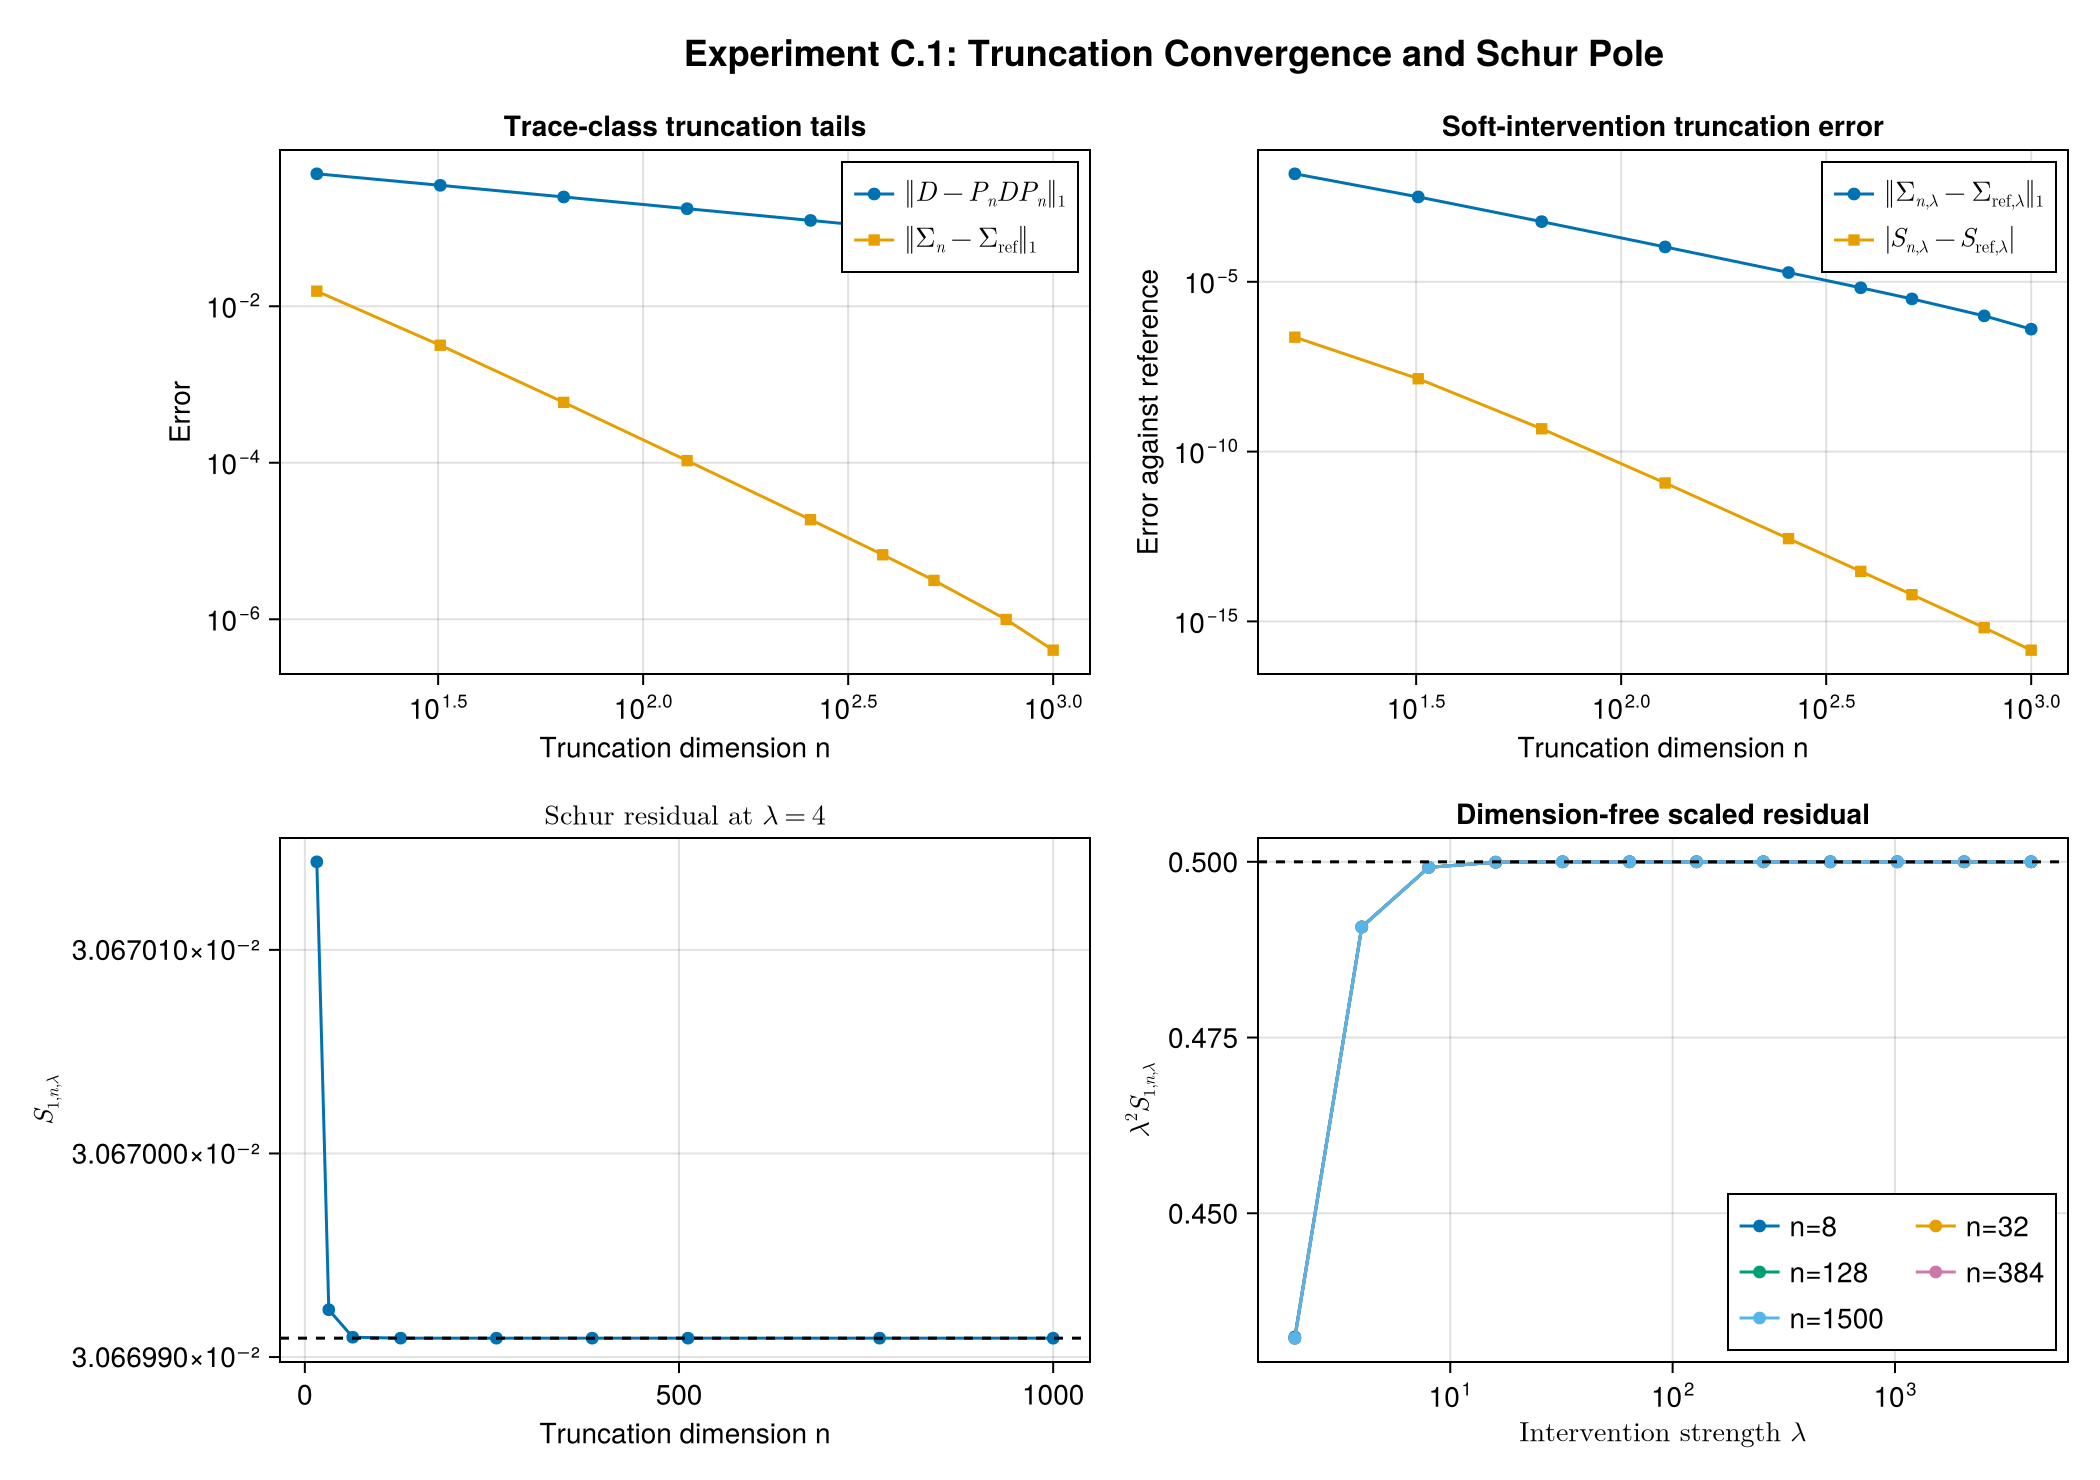
\includegraphics[width=0.8\textwidth]{figures/truncation_convergence_validation.png}
  \caption{Experiment~C.1. Trace-norm and residual errors decay in $n$; the extrapolated $m_2^{\mathrm{Schur},(1000)}$ differs from $\varepsilon_0/2$ by $6.87\times10^{-14}$.}
  \label{fig:truncation}
\end{figure}



\subsection{Exact Variance Normalization Diagnostic}
\label{app:experiments:ablation}

We validate the exact variance normalization of Proposition~\ref{prop:exact_calibration} in its decoupled reference channel. With incoming arrows cut and off-diagonal drift coupling set to zero, the target covariance is exactly $\Sigma_{\lambda,22} = d_\lambda / (2\lambda)$. Four candidate target-diffusion families are tested:
\begin{enumerate}
  \item \textbf{Canonical:} $d_\lambda=\varepsilon_0/\lambda$.
  \item \textbf{Slow:} $d_\lambda=\varepsilon_0$.
  \item \textbf{Fast:} $d_\lambda=\varepsilon_0/\lambda^2$.
  \item \textbf{Perturbed:} $d_\lambda=(\varepsilon_0/\lambda)(1+\lambda^{-2})$.
\end{enumerate}

All evaluations are performed in Julia using 256-bit \texttt{BigFloat} arithmetic. A probe at $\lambda=2^{100}$ resolves the nonzero finite-scale defect of the perturbed family.

\begin{table}[h]
  \centering
  \caption{Exact-calibration ablation. Only the canonical family satisfies the exact finite-$\lambda$ covariance condition.}
  \label{tab:ablation}
  \begin{tabular}{lll}
    \toprule
    Family & $\lambda d_\lambda/\varepsilon_0$ & defect $|2\lambda^2\Sigma_{\lambda,kk}/\varepsilon_0-1|$ \\
    \midrule
    Canonical & $1$ & $0$ \\
    Slow & $\lambda$ & $\lambda-1 \to \infty$ \\
    Fast & $\lambda^{-1}$ & $|1-\lambda^{-1}| \to 1$ \\
    Perturbed & $1+\lambda^{-2}$ & $\lambda^{-2}$ \\
    \bottomrule
  \end{tabular}
\end{table}

\begin{figure}[h]
  \centering
  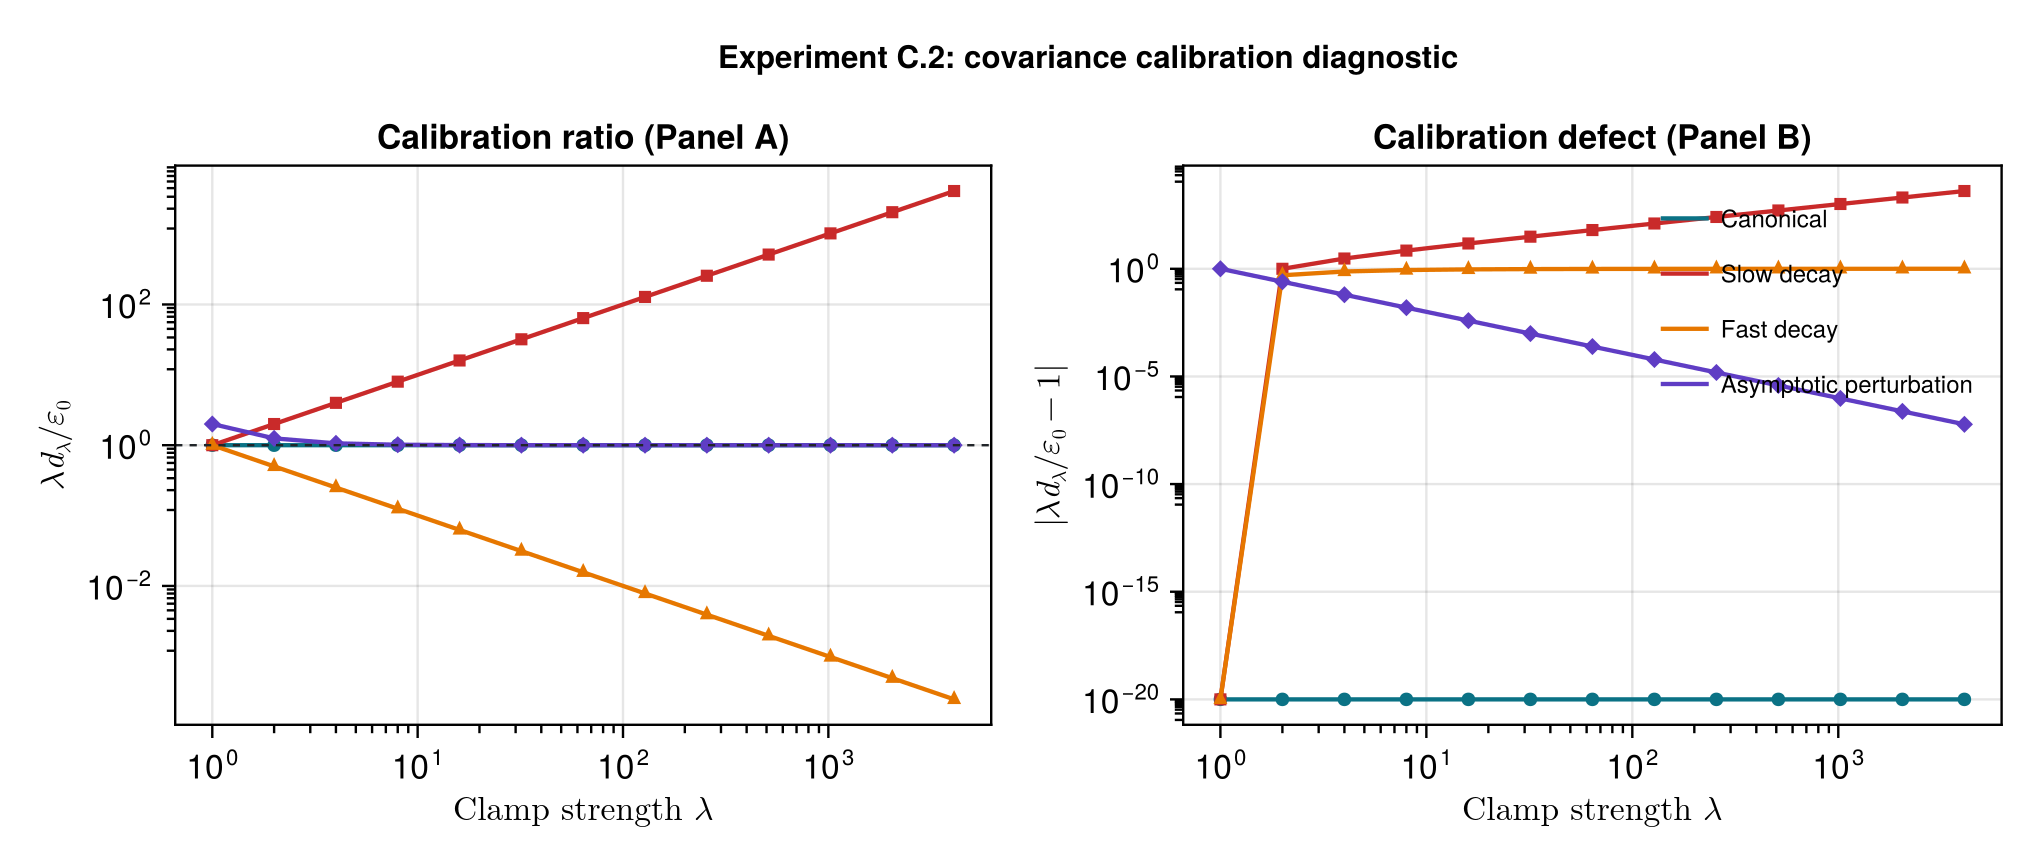
\includegraphics[width=0.9\textwidth]{figures/ablation_combined.png}
  \caption{Experiment~C.2. The perturbed family has the correct limiting ratio but fails the exact finite-$\lambda$ covariance condition. Exact zero defects are displayed at $10^{-20}$.}
  \label{fig:ablation}
\end{figure}



\subsection{Gaussian Finite-Part Functional in a Three-Node Chain}
\label{app:experiments:three_node}

We evaluate the Gaussian renormalized finite-part functional $\mathfrak{J}_\lambda$ on a three-node linear Ornstein--Uhlenbeck SDE:
\begin{equation}
  X_1 \to X_2 \to X_3,
\end{equation}
where $X_2$ is the target coordinate subject to regularized conditioning of strength $\lambda \in \{2^1, \dots, 2^{12}\}$, with $x_2^* = 0$ and $\varepsilon_0 = 1$. The drift and diffusion operators are:
\begin{equation}
  A_\lambda = \begin{pmatrix} -1 & 0 & 0 \\ 0 & -\lambda & 0 \\ 0 & a_{32} & -1 \end{pmatrix}, \qquad D_\lambda = \operatorname{diag}(1, \varepsilon_0/\lambda, 1).
\end{equation}
The target mean forcing $b_2$ controls the target mean shift $m_{\lambda,2} = b_2/\lambda$.
We evaluate three Gaussian cases:
\begin{enumerate}
  \item \textbf{Case A (Decoupled-centered):} $a_{32} = 0, b_2 = 0$. Here $\mathfrak{J}_\lambda = 0$ exactly for all $\lambda$.
  \item \textbf{Case B (Coupled-centered):} $a_{32} = 1, b_2 = 0$. The coupling causes leakage $\Sigma_{23} \neq 0$, but the centering gives $\mathfrak{J}_\lambda = O(\lambda^{-4}) \to 0$.
  \item \textbf{Case C (Coupled-off-centered):} $a_{32} = 1, b_2 = 1$. The deterministic forcing causes mean shift $m_{\lambda,2} = 1/\lambda$, yielding $\mathfrak{J}_\lambda \to b_2^2/\varepsilon_0 = 1$.
\end{enumerate}
All evaluations are performed in Julia using 256-bit \texttt{BigFloat} arithmetic, showing that the Schur residual $\lambda^2 S_{2,\lambda}$ converges to $1/2$ in all cases, while $\mathfrak{J}_\lambda$ exhibits the exact zero, $O(\lambda^{-4})$ decay, and convergence to 1 behavior respectively.

\begin{figure}[h]
  \centering
  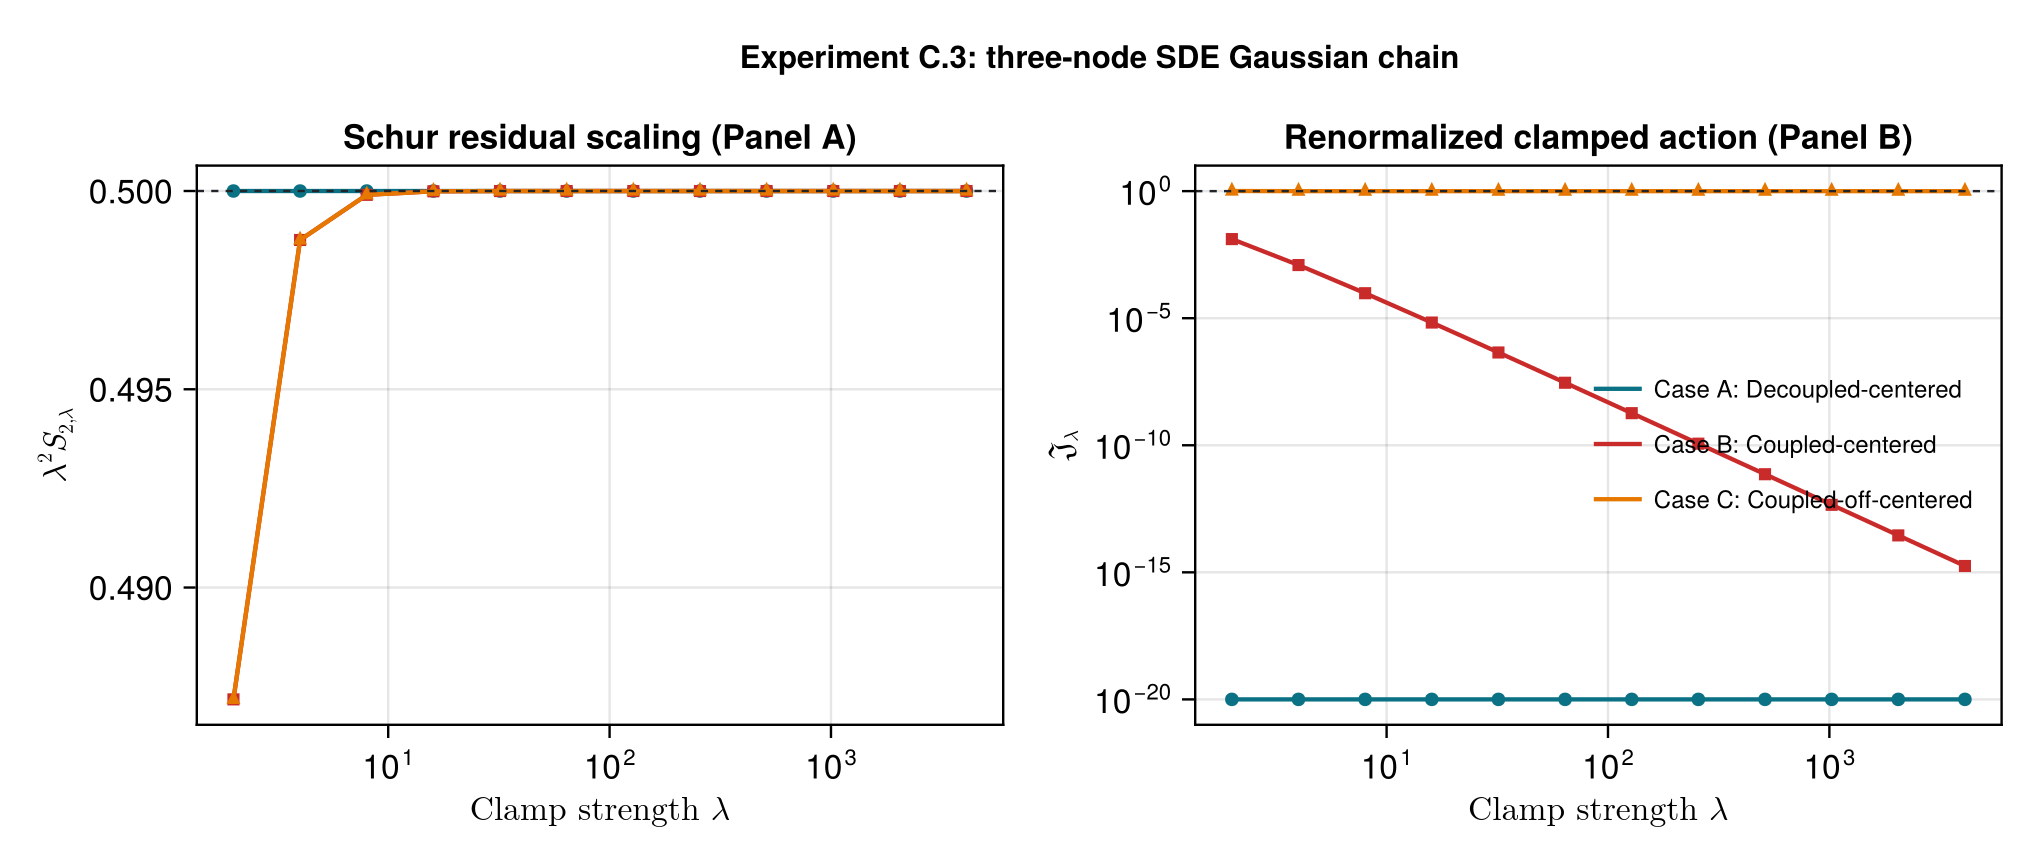
\includegraphics[width=0.9\textwidth]{figures/three_node_gaussian_chain.png}
  \caption{Experiment~C.3. The panels show $\lambda^2S_{2,\lambda}\to0.5$ and the three finite-part regimes: exact zero, $O(\lambda^{-4})$ decay, and convergence to $1$. Exact zeros are displayed at $10^{-20}$.}
  \label{fig:three_node}
\end{figure}



\subsection{Numerical Precision Audit}
\label{app:numerical_precision}

At $n=256$, we recompute representative C.1 Schur residuals using IEEE 754 \texttt{Float64} and 256-bit Julia \texttt{BigFloat} arithmetic with the same covariance equation and Schur solve.

\begin{table}[h]
  \centering
  \caption{Precision audit at $n=256$; $S_{256}$ uses 256-bit \texttt{BigFloat}.}
  \label{tab:precision_audit}
  \begin{tabular}{rrrr}
    \toprule
    $\lambda$ & $\kappa_2(\Sigma_{II})$ &
    $|\lambda^2 S-\tfrac12|$ &
    $|S_{64}-S_{256}|/|S_{256}|$ \\
    \midrule
    $4$ & $2.97\times10^6$ & $3.45\times10^{-1}$ & $6.50\times10^{-16}$ \\
    $64$ & $9.14\times10^5$ & $1.13\times10^{-3}$ & $3.48\times10^{-17}$ \\
    $4096$ & $9.14\times10^5$ & $9.20\times10^{-10}$ & $5.54\times10^{-17}$ \\
    \bottomrule
  \end{tabular}
\end{table}

For the five-point extrapolation of $m_2^{\mathrm{Schur},(256)}$,
\texttt{Float64} and \texttt{BigFloat} differ by
$9.98\times10^{-17}$; finite-$\lambda$ remainder, not rounding, governs
the observed distance to the limiting constant.



\begin{remark}[Block-decoupling error suppression]
\label{rmk:block_decoupling_error}
The sub-machine-epsilon agreement between \texttt{Float64} and \texttt{BigFloat} in Table~\ref{tab:precision_audit} is not coincidental; it is a direct consequence of the block-triangular structure established in this paper. Under the block-decoupled conditioning, the drift matrix takes the form
\begin{equation}
  \mathcal{A}^{(\lambda)}=\begin{pmatrix}-\lambda&0\\a_{Ik}&A_{II}\end{pmatrix},
\end{equation}
so the operator Lyapunov equation decomposes into three sub-problems:
\begin{enumerate}
  \item The target block $\Sigma_{\lambda,kk}=d_\lambda/(2\lambda)$ is solved by a single scalar division, incurring at most $\frac{1}{2}\epsilon_{\mathrm{machine}}$ relative rounding error (IEEE~754 round-to-nearest).
  \item The cross-covariance $\Sigma_{\lambda,Ik}$ satisfies $|\Sigma_{\lambda,Ik}|_{Q_0}=O(\lambda^{-3})$ by \eqref{eq:cross_energy_bound}, so the absolute rounding error in the cross block is $O(\lambda^{-3}\epsilon_{\mathrm{machine}})$.
  \item The free block $\Sigma_{\lambda,II}$ is a standard Lyapunov solution with absolute error $O(\epsilon_{\mathrm{machine}}\|\Sigma_{\lambda,II}\|)$.
\end{enumerate}
When the Schur complement is assembled as $S_{k,\lambda}=\Sigma_{\lambda,kk}-R_\lambda$, the subtracted variational term satisfies $R_\lambda=O(\lambda^{-6})$ (Theorem~\ref{thm:inf_cancellation}), which is negligible compared to $\Sigma_{\lambda,kk}=O(\lambda^{-2})$. The rounding error in $S_{k,\lambda}$ is therefore dominated by the error in $\Sigma_{\lambda,kk}$ alone, yielding a Schur-level rounding budget of $O(\epsilon_{\mathrm{machine}}\cdot\Sigma_{\lambda,kk})$ rather than the na\"ive $O(\epsilon_{\mathrm{machine}}\cdot\|\Sigma_{\lambda,II}^{-1}\|\cdot\|\Sigma_{\lambda,Ik}\|^2)$ that one would expect without block decoupling.

In short, the block-triangular structure converts what would be a catastrophically ill-conditioned Schur computation into a well-conditioned scalar computation plus negligible corrections. The observed \texttt{Float64}--\texttt{BigFloat} agreement at $O(10^{-17})$ is the numerical signature of this structural decoupling.
\end{remark}

\subsection{The dichotomy of dual geometries}
\label{sec:numerical:dichotomy}

To illustrate the simultaneous collapse and survival of the unified geometry under singular conditioning, we track the target scaling metrics on a 3-node serial OU chain under target coordinate conditioning on $X_2$ ($\varepsilon_0 = 1$). 
The 0th-order normal metric is extracted via the pull-back Jacobian:
\begin{equation}
  g_{\lambda,\text{normal}} := \lambda^{-2}S_{K,\lambda}^{-1}.
\end{equation}
In a log-log evaluation over $\lambda \in [2^1, 2^{20}]$, the normal metric $g_{\lambda,\text{normal}}$ instantly stabilizes to the horizontal plateau $2/\varepsilon_0$. Conversely, the unrenormalized horizontal lift response $g_\lambda^{\text{bulk}} = A_\lambda^{-2}R_\lambda$ collapses strictly at a slope of $-2$ ($O(\lambda^{-2}) \to 0$). Upon RFIM rescaling ($\lambda^2$), the 1st-order metric locks onto a distinct constant offset perfectly matching the theoretical Cameron--Martin limit $\|a_{Ik}\|_{Q_0^{-1}}^2$.

\begin{figure}[htbp]
  \centering
  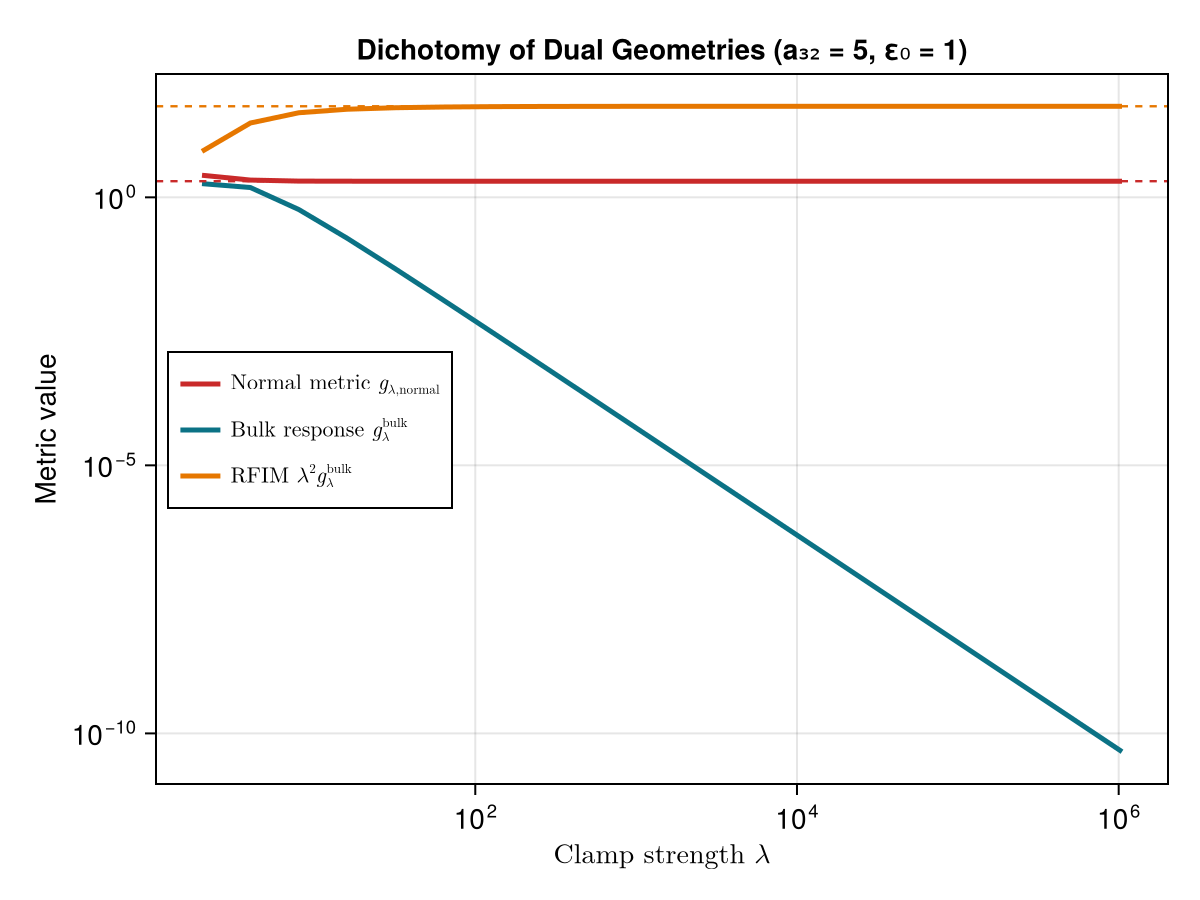
\includegraphics[width=0.75\textwidth]{figures/dichotomy_geometries.png}
  \caption{Dichotomy of dual geometries for the 3-node serial Gaussian chain under target coordinate conditioning on $X_2$ ($\varepsilon_0 = 1$, $a_{32} = 5$). The 0th-order normal metric $g_{\lambda,\text{normal}}$ (red) instantly stabilizes at the horizontal plateau $2/\varepsilon_0 = 2$, showing the survival of the boundary geometry. The unrenormalized horizontal lift response $g_\lambda^{\text{bulk}}$ (blue) collapses strictly at a slope of $-2$ as $O(\lambda^{-2})$. Rescaling the bulk response by $\lambda^2$ yields the 1st-order metric (orange), which locks onto the non-zero Cameron--Martin limit $\|a_{Ik}\|_{Q_0^{-1}}^2 = 2 a_{32}^2 = 50$.}
  \label{fig:dichotomy_geometries}
\end{figure}

The log-log scaling plot in Figure~\ref{fig:dichotomy_geometries} demonstrates that while the horizontal connection collapses, the boundary normal geometry survives intact, and the renormalized 1st-order perturbation retains the coupling invariant.



\subsection{Orthogonal independence of normal geometry and horizontal lift}
\label{sec:numerical:orthogonal}

To verify that the 0th-order boundary normal metric and the 1st-order horizontal lift quantify logically independent responses, we preserve the exact target scaling ($\varepsilon_0 = 1$) while toggling the outgoing cross-coupling $a_{32}$. 
As demonstrated in Table~\ref{tab:orthogonal_independence}, modifying the off-diagonal leakage strictly varies the 1st-order residual while leaving the normal geometry universally preserved.

\begin{table}[htbp]
  \centering
  \caption{Verification of orthogonal decoupling of normal geometry and horizontal lift}
  \label{tab:orthogonal_independence}
  \begin{tabular}{lccc}
    \toprule
    Environment & Coupling $a_{32}$ & 0th-order Metric & 1st-order Metric (RFIM) \\
    \midrule
    \textbf{Decoupled} & $0$ & $2.00000000$ & $0.00000000$ \\
    \textbf{Coupled}   & $5$ & $2.00000000$ & $49.99990463$ \\
    \bottomrule
  \end{tabular}
\end{table}

Table~\ref{tab:orthogonal_independence} numerically proves the conceptual core: the 0th-order normal metric is uniquely calibrated by the unperturbed evidence noise scale, while the 1st-order horizontal lift is exclusively governed by the off-diagonal Cameron--Martin connection energy.



\subsection{Convergence to the Mahalanobis normal well}
\label{sec:numerical:mahalanobis}

Because the background regularized-conditioning measure constitutes a Gaussian location family with covariance invariant to the evidence offset $b$, the blow-up Fisher metric matrix $G_{\lambda,K} := \lambda^{-2}S_{K,\lambda}^{-1}$ remains rigidly constant with respect to $b$ at every finite $\lambda$, yielding a purely flat geometry ($\Gamma = R \equiv 0$).
We verify the constant convergence rate of the matrix geometry in a target block of $|K|=2$. As $\lambda \to \infty$, the finite-$\lambda$ flat quadratic cost contours converge unconditionally to the limiting Mahalanobis well governed by the Schur second-order coefficient matrix $E_0$:
\begin{equation}
  \mathfrak{D}_\lambda^{\text{FP}}(b,0) = \frac{1}{2}b^\top G_{\lambda,K} b \longrightarrow \mathfrak{D}^{\text{FP}}(b,0) = b^\top E_0^{-1} b.
\end{equation}
Evaluation confirms that the distance between the intermediate geometries decays in Frobenius norm as $\|G_{\lambda,K} - 2E_0^{-1}\|_F = O(\lambda^{-4})$.

\begin{figure}[htbp]
  \centering
  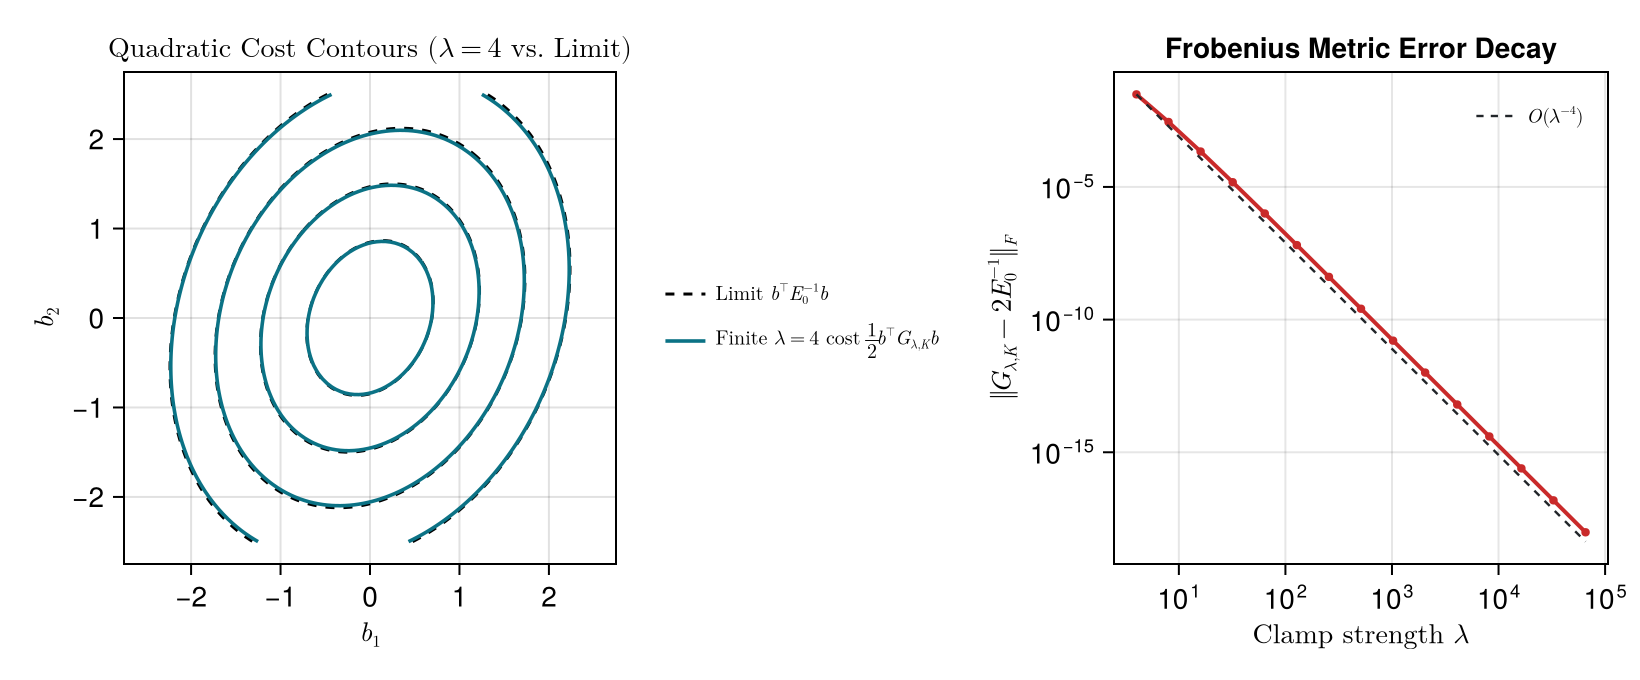
\includegraphics[width=0.95\textwidth]{figures/mahalanobis_well_convergence.png}
  \caption{Convergence of the finite-$\lambda$ quadratic cost contours to the limiting Mahalanobis normal well for target block $|K|=2$ with off-diagonal coupling. \textbf{Left (Panel A):} Contours of the finite-$\lambda$ cost $\frac{1}{2}b^\top G_{\lambda,K} b$ at $\lambda = 4$ (solid blue lines) overlaid with the contours of the limiting Mahalanobis cost $b^\top E_0^{-1} b$ (dashed black lines), demonstrating close alignment even at a low regularizer strength. \textbf{Right (Panel B):} Log-log plot of the Frobenius norm error $\|G_{\lambda,K} - 2E_0^{-1}\|_F$ (solid red line with markers) versus the regularizer strength $\lambda \in [2^2, 2^{16}]$, running in parallel with the theoretical $O(\lambda^{-4})$ slope reference (dashed black line).}
  \label{fig:mahalanobis_well_convergence}
\end{figure}

The contour comparison in Figure~\ref{fig:mahalanobis_well_convergence} (Panel A) demonstrates that the quadratic geometry of the blow-up divergence rapidly converges to the limiting Mahalanobis well. The error decay in Figure~\ref{fig:mahalanobis_well_convergence} (Panel B) confirms that the distance between the intermediate and limiting geometries in Frobenius norm decays strictly at the Schur geometric rate of $O(\lambda^{-4})$. Thus, the singularity does not generate curvature; it selects a finite flat metric. This flatness is not a vacuous triviality, but a structural consequence of the location family under regularized conditioning, with the hard-limit topological clamp rigorously preserving the displacement flatness.



\end{document}
